% From https://github.com/UWIT-IAM/UWThesis
\documentclass[print]{nuthesis}
\usepackage{amssymb, amsthm, amsmath, amsfonts}
\usepackage{wasysym}
\usepackage{mathrsfs}
% \usepackage{hyperref}
\usepackage{graphicx}
\usepackage{lineno}
\usepackage[colorinlistoftodos]{todonotes}
\usepackage{listings}
%\usepackage{breqn}
\usepackage{cancel, enumerate}
\usepackage{rotating, environ}
\usepackage{caption}
\usepackage{subcaption}
\usepackage[inline]{enumitem}
\usepackage{dirtree}
\usepackage{framed}

\newtheorem{thm}{Theorem}
\newtheorem{defn}{Definition}
\newtheorem{prop}{Proposition}
\newtheorem{lemma}{Lemma}
\newtheorem{cor}{Corollary}

% Syntax highlighting #22
\usepackage{color}
\usepackage{fancyvrb}
\newcommand{\VerbBar}{|}
\newcommand{\VERB}{\Verb[commandchars=\\\{\}]}
\DefineVerbatimEnvironment{Highlighting}{Verbatim}{commandchars=\\\{\}}
% Add ',fontsize=\small' for more characters per line
\usepackage{framed}
\definecolor{shadecolor}{RGB}{248,248,248}
\newenvironment{Shaded}{\begin{snugshade}}{\end{snugshade}}
\newcommand{\AlertTok}[1]{\textcolor[rgb]{0.94,0.16,0.16}{#1}}
\newcommand{\AnnotationTok}[1]{\textcolor[rgb]{0.56,0.35,0.01}{\textbf{\textit{#1}}}}
\newcommand{\AttributeTok}[1]{\textcolor[rgb]{0.13,0.29,0.53}{#1}}
\newcommand{\BaseNTok}[1]{\textcolor[rgb]{0.00,0.00,0.81}{#1}}
\newcommand{\BuiltInTok}[1]{#1}
\newcommand{\CharTok}[1]{\textcolor[rgb]{0.31,0.60,0.02}{#1}}
\newcommand{\CommentTok}[1]{\textcolor[rgb]{0.56,0.35,0.01}{\textit{#1}}}
\newcommand{\CommentVarTok}[1]{\textcolor[rgb]{0.56,0.35,0.01}{\textbf{\textit{#1}}}}
\newcommand{\ConstantTok}[1]{\textcolor[rgb]{0.56,0.35,0.01}{#1}}
\newcommand{\ControlFlowTok}[1]{\textcolor[rgb]{0.13,0.29,0.53}{\textbf{#1}}}
\newcommand{\DataTypeTok}[1]{\textcolor[rgb]{0.13,0.29,0.53}{#1}}
\newcommand{\DecValTok}[1]{\textcolor[rgb]{0.00,0.00,0.81}{#1}}
\newcommand{\DocumentationTok}[1]{\textcolor[rgb]{0.56,0.35,0.01}{\textbf{\textit{#1}}}}
\newcommand{\ErrorTok}[1]{\textcolor[rgb]{0.64,0.00,0.00}{\textbf{#1}}}
\newcommand{\ExtensionTok}[1]{#1}
\newcommand{\FloatTok}[1]{\textcolor[rgb]{0.00,0.00,0.81}{#1}}
\newcommand{\FunctionTok}[1]{\textcolor[rgb]{0.13,0.29,0.53}{\textbf{#1}}}
\newcommand{\ImportTok}[1]{#1}
\newcommand{\InformationTok}[1]{\textcolor[rgb]{0.56,0.35,0.01}{\textbf{\textit{#1}}}}
\newcommand{\KeywordTok}[1]{\textcolor[rgb]{0.13,0.29,0.53}{\textbf{#1}}}
\newcommand{\NormalTok}[1]{#1}
\newcommand{\OperatorTok}[1]{\textcolor[rgb]{0.81,0.36,0.00}{\textbf{#1}}}
\newcommand{\OtherTok}[1]{\textcolor[rgb]{0.56,0.35,0.01}{#1}}
\newcommand{\PreprocessorTok}[1]{\textcolor[rgb]{0.56,0.35,0.01}{\textit{#1}}}
\newcommand{\RegionMarkerTok}[1]{#1}
\newcommand{\SpecialCharTok}[1]{\textcolor[rgb]{0.81,0.36,0.00}{\textbf{#1}}}
\newcommand{\SpecialStringTok}[1]{\textcolor[rgb]{0.31,0.60,0.02}{#1}}
\newcommand{\StringTok}[1]{\textcolor[rgb]{0.31,0.60,0.02}{#1}}
\newcommand{\VariableTok}[1]{\textcolor[rgb]{0.00,0.00,0.00}{#1}}
\newcommand{\VerbatimStringTok}[1]{\textcolor[rgb]{0.31,0.60,0.02}{#1}}
\newcommand{\WarningTok}[1]{\textcolor[rgb]{0.56,0.35,0.01}{\textbf{\textit{#1}}}}

%% https://github.com/rstudio/rmarkdown/issues/1649
\newlength{\cslhangindent}
\setlength{\cslhangindent}{1.5em}
\newenvironment{CSLReferences}[2]%
{\setlength{\parindent}{0pt}%
\everypar{\setlength{\hangindent}{\cslhangindent}}\ignorespaces}%
{\par}

% fix for pandoc 1.14
\providecommand{\tightlist}{%
  \setlength{\itemsep}{0pt}\setlength{\parskip}{0pt}}

%% something about tables, from https://github.com/ismayc/thesisdown/issues/122
\usepackage{calc}

%% for copyright symbol
\usepackage{textcomp}

%% to allow to rotate pages to landscape
\usepackage{lscape}
%% to adjust table column width
\usepackage{tabularx}

% suppress bottom page numbers on first page of each chapter
% because they overlap with text
\usepackage{etoolbox}
\patchcmd{\chapter}{plain}{empty}{}{}

%% for more attractive tables
\usepackage{booktabs}
\usepackage{longtable}


\usepackage{graphicx}


% Double spacing, if you want it.
\def\dsp{\def\baselinestretch{2.0}\large\normalsize}
% \dsp

% If the Grad. Division insists that the first paragraph of a section
% be indented (like the others), then include this line:
\usepackage{indentfirst}

%%%%%%%%%%%%%%%%%%
% If you want to use "sections" to partition your thesis
% un-comment the following:
%
% \counterwithout{section}{chapter}
% \setsecnumdepth{subsubsection}
% \def\sectionmark#1{\markboth{#1}{#1}}
% \def\subsectionmark#1{\markboth{#1}{#1}}
% \renewcommand{\thesection}{\arabic{section}}
% \renewcommand{\thesubsection}{\thesection.\arabic{subsection}}
% \makeatletter
% \let\l@subsection\l@section
% \let\l@section\l@chapter
% \makeatother

\renewcommand{\thetable}{\arabic{table}}
\renewcommand{\thefigure}{\arabic{figure}}

%%%%%%%%%%%%%%%%%%


%% Stuff from https://github.com/suchow/Dissertate

% The following line would print the thesis in a postscript font

% \usepackage{natbib}
% \def\bibpreamble{\protect\addcontentsline{toc}{chapter}{Bibliography}}

\setcounter{tocdepth}{1} % Print the chapter and sections to the toc
% controls depth of table of contents (toc): 0 = chapter, 1 = section, 2 = subsection

\usepackage{natbib}


% commands and environments needed by pandoc snippets
% extracted from the output of `pandoc -s`
%% Make R markdown code chunks work
\usepackage{array}
\usepackage{amssymb,amsmath}
\usepackage{ifxetex,ifluatex}
\ifxetex
  \usepackage{fontspec,xltxtra,xunicode}
  \defaultfontfeatures{Mapping=tex-text,Scale=MatchLowercase}
\else
  \ifluatex
    \usepackage{fontspec}
    \defaultfontfeatures{Mapping=tex-text,Scale=MatchLowercase}
  \else
    \usepackage[utf8]{inputenc}
  \fi
\fi
\usepackage{color}
\usepackage{fancyvrb}


\ifxetex
  \usepackage[setpagesize=false, % page size defined by xetex
              unicode=false, % unicode breaks when used with xetex
              xetex,
              colorlinks=true,
              linkcolor=blue]{hyperref}
\else
  \usepackage[unicode=true,
              colorlinks=true,
              linkcolor=blue]{hyperref}
\fi
\hypersetup{breaklinks=true, pdfborder={0 0 0}}
\setlength{\parindent}{20pt}
\setlength{\parskip}{6pt plus 2pt minus 1pt}
\setlength{\emergencystretch}{3em}  % prevent overfull lines
\setcounter{secnumdepth}{2} %% controls section numbering, e.g. 1 or 1.2, or 1.2.3



%  ----  Text Colors  ------------------------------------------
%
% Assign colors to writers for review
%
\newcommand{\db}[1]{{\textcolor{blue}{#1}}}
\newcommand{\svp}[1]{{\textcolor{RedOrange}{#1}}}
\newcommand{\cochaircol}[1]{{\textcolor{Green}{#1}}}
%


%  --- Code chunk font size -----------------------------------------------
% https://stackoverflow.com/questions/38323331/code-chunk-font-size-in-beamer-with-knitr-and-latexhttps://stackoverflow.com/questions/38323331/code-chunk-font-size-in-beamer-with-knitr-and-latex

%% change fontsize of R code
\let\oldShaded\Shaded
\let\endoldShaded\endShaded
\renewenvironment{Shaded}{\footnotesize\oldShaded}{\endoldShaded}

%% change fontsize of output
\let\oldverbatim\verbatim
\let\endoldverbatim\endverbatim
\renewenvironment{verbatim}{\footnotesize\oldverbatim}{\endoldverbatim}


\begin{document}
% \linenumbers{}
%% Start formatting the first few special pages
%% frontmatter is needed to set the page numbering correctly
\frontmatter
%% from thesisdown
% To pass between YAML and LaTeX the dollar signs are added by CII
\title{An investigation into how well dashboards using open-source data support statistical visual inference for naive users.}
\author{Denise Renee Bradford}
\adviser{Susan R. VanderPlas, Ph.D}
% \adviserAbstract{}
\major{Statistics}
\degreemonth{Month}
\degreeyear{Year}
% \copyrightpage
%%
%% For most people the defaults will be correct, so they are commented
%% out. To manually set these, just uncomment and make the needed
%% changes.
%% \college{Your college}
%% \city{Your City}
%%
%% For most people the following can be changed with a class
%% option. To manually set these, just uncomment the following and
%% make the needed changes.
%% \doctype{Thesis or Dissertation}
%% \degree{Your degree}
%% \degreeabbreviation{Your degree abbr.}
%%
%% Now that we know everything we need, we can generate the title page
%% itself.
%%
\maketitle


\begin{abstract}
    In the modern digital era, the exponential growth of data has forced the development and use of user-friendly tools to visualize this data, most notably dashboards. Dashboards are essential for interpreting complex datasets and supporting well-informed decision-making because they are interactive visual representation platforms. This dissertation examines how well these dashboards, in particular those that use open-source data, enable statistical visual inference for users, or ``naive users,'' who have little or no experience with data analytics.
    Due to its democratized nature, open-source data has become a significant source of information, assisting a variety of industries from public health to urban planning. Utilizing this data in dashboards can be extremely beneficial for the general public, especially for those without a thorough understanding of data interpretation. The difficulty, however, lies in creating dashboards that can not only effectively present data but also help uninformed users make accurate statistical inferences without misunderstanding.
\end{abstract}

%% Optional
\begin{copyrightpage}
\end{copyrightpage}

%% Optional
\begin{dedication}
Dedicated to\ldots{}
\end{dedication}

%%%%%%%%%%%%%%%%%%%
% Acknowledgments
%%%%%%%%%%%%%%%%%%%
\begin{acknowledgments}
Thank you to all my people!
\end{acknowledgments}
%%%%%%%%%%%%%%%%%%%

%%%%%%%%%%%%%%%%%%%
% Grant Information
%%%%%%%%%%%%%%%%%%%
% \begin{grantinfo}
%     % Add any grant info here
% \end{grantinfo}

%%%%%%%%%%%%%%%%%%%
% ToC
%%%%%%%%%%%%%%%%%%%
\tableofcontents

%%%%%%%%%%%%%%%%%%%
% List of Figures
%%%%%%%%%%%%%%%%%%%
\listoffigures
\listoftables

%%%%%%%%%%%%%%%%%%%
% Start of the document
%%%%%%%%%%%%%%%%%%%
\mainmatter


\hypertarget{introduction}{%
\chapter{Introduction}\label{introduction}}

Our data-driven modern civilization now depends heavily on the ability to precisely evaluate and exploit huge and complex datasets, especially in small rural towns where resources are often sparse.
This dissertation aims to make big datasets more understandable and useful by utilizing three related innovations: generalized parallel coordinate plots (GPCPs), reliable ways to look at missing data, and efficient methods to elaborate on the detection of unusual trends.
Each priority area is key for improving the GPCP technique to enable thorough and accurate data analysis across various datasets.

The accuracy of data interpretation is highest when dealing directly with numerical values or one-dimensional visual representations (Spence, 1990).
That is becoming more and more impractical. The size and dimensionality of datasets are increasing.
In order to make judgments based on data, it is necessary to find methods of simplifying and consolidating datasets without sacrificing significant information.
Often, a data visualization, such as a graph or table, serves as a go-between step between raw data and an observer's decision-making process. A data visualization is the visual depiction of information.
Essentially, it is an effort to effectively communicate synthesized data pieces in a way that is easy for an observer to understand and evaluate.

For high-dimensional data, parallel coordinate plots (PCPs) are a common visualization tool whereby data points are shown as lines intersecting each axis, therefore indicating a dimension.
Conventional PCP hinders its interpretability by having clutter and overlapping lines while handling big datasets. By including methods such as axis reordering, bundling, and dimensionality reduction to solve these problems, generalized parallel coordinate plots (GPCPs) expand the conventional PCP.
These improvements in clarity and usability of PCPs by means of data pattern highlighting and visual clutter reduction help Heinrich and Weiskopf (2013), for example, present several approaches to bundle comparable trajectories in GPCPs, so minimizing overlap and improving pattern identification; Johannsen et al.~(2012) address the advantages of dynamic axis reordering to highlight different data characteristics.

Stimulus-responsive attention is typically triggered by a certain category, where an observer learns that one element of the stimulus contains valuable information about the most promising location to search for additional information in order to make an accurate judgment.
Greensmith's ``Personal Equation of Interaction'' investigates personal variations in cognitive and perceptual capacity when using sophisticated visual interfaces (Greensmith, 2016).
This theory emphasizes the need of human characteristics in understanding and classifying composite glyphs, graphical elements expressing multidimensional data.
Applied to generalized parallel coordinate plots (GPCPs), it underlines the requirement of considering individual cognitive and perceptual variances since these influence data interpretation accuracy and efficiency. Generalized parallel coordinate charts display many dimensions within a single glyph.

Overall, this dissertation addresses theoretical and practical gaps within the existing literature and offers tangible improvements to GPCP's functionality.
By enhancing the treatment of missing data, refining outlier detection, and upgrading statistical methodologies, this research aims to extend GPCP's applicability across diverse research fields, ultimately facilitating more accurate and insightful data analysis.
Through a mix of theoretical expansion, algorithm development, and practical application, the enhancements proposed herein seek to advance the field of data visualization significantly.

\hypertarget{cognition-models-and-data-visualization}{%
\section{Cognition Models and Data Visualization}\label{cognition-models-and-data-visualization}}

Data visualization professionals are impacted by advancements in cognitive science, as evidenced by multiple research studies (Healey \& Enns, 2011; Hegarty, 2011; Crapo, Waisel, Wallace \& Willemain, 2000). Additionally, cognitive scientists contribute to developing ideas about data visualization (e.g., Kosslyn, 2006; Green, Ribarsky \& Fisher, 2009; Pinker, 1990; Lewandowsky \& Spence, 1989).

However, data visualization models primarily clarify the connection between users and the display rather than describe the cognitive processes involved in response to data visualizations.

The following will present a concise overview of data visualization methods that assert the influence of the cognitive system.

This is done partly to discover patterns and demonstrate the current level of abstraction in comprehending the connection between the observer and the data. Most models that establish a connection between the observer and data in data visualization do not.

These experiments manipulate low-level visual features not explicitly incorporated into current data visualization models. Several of the theories below show the absence of a clear relationship between perception and cognition.

Data visualization models are generally abstract, process-oriented descriptions of how the user interacts with the image.
Waisal, Wallace \& Willemain (1999) put forth a data visualization theory that proposes mental models as how observers comprehend the world.
Mental models are cognitive constructs believed by some to serve as the foundation for relational reasoning, as proposed by Johnson-Laird in 1983 and further supported by Byrne and Johnson-Laird in 1989. Mental models have three essential elements: understanding, description, and validation.
The theory of data visualization proposed by Waisal and colleagues corresponds to the initial stage of a mental model, where information is encoded, and the cognitive system readies itself for further elaboration.
The model proposed by Waisal et al.~describes a series of processes that an observer must follow to synchronize their mental representation of the information in the display with the actual display.
The system takes the observer's understanding of the data as input and generates a response that can be verified.
The initial step of the Waisal et al.~model involves constructing a mental representation based on the observers' understanding of the data visualization.
Subsequently, an observer selects a certain perspective from this mental model and accurately reproduces it based on the observed graph.
To make progress, the observer needs to assess three things: 1) if the visualization accurately corresponds to the model view, 2) if the visualization is consistent with the mental model, and 3) if the view and visualization are feasible when taking external factors into account.
Once all three conditions are satisfied, the observer proceeds to the validation stage of the mental model.
If any criteria are not satisfied, the mental model is revised, and the view is derived based on the revised mental model.

The practical implications of the research are evident in the data obtained from the think-aloud technique and mouse-tracking.
These findings, as reported by Waisel et al.~(1999), indicate that viewers do utilize certain steps in the process of comprehending the data visualization.
While the sequence of stages was not easily identifiable from the observed data, the authors propose that suggesting separate steps was beneficial for isolating sub-processes and gaining a clearer grasp of the description aspect involved in constructing a mental model.
This insight can be valuable in designing more effective data visualizations that align with the cognitive processes of the viewers.

Pinker's theory (1990) states that the mind is made of a collection of separate, natural mental modules that were developed to manage particular kinds of data and activities.
This thoery offers a unique perspective on the cognitive components involved in understanding graphs at a higher level.
It includes a matching process, which utilizes a graph schema of the suitable type, a message assembly that converts visual information into conceptual information, an interrogation stage where additional information is extracted from the graph if necessary, and finally an inferential process where decisions are made or insights are generated.

Each of these four procedures involves highly intricate matters.
The conversion of visual input into a conceptually meaningful form is a complex task, yet it is encapsulated in a single step in this model.
However, this is not necessarily a drawback.
If we consider this theory as a means to effectively break down the challenge of data visualization into smaller, more manageable components, then it is beneficial to divide an overwhelmingly large problem (how individuals comprehend graphs) into more meaningful sub-problems, such as understanding how people transform visual data into meaningful information.
Pinker defines the matching process as a component of ``cognitive fit'', which Vessey and his colleagues have separately investigated as a distinct problem.

For people to understand the data, how the information is presented is important.
Traditionally, scatterplots are great for showing how two variables are related, bar graphs are great for showing a key property of multiple levels of a single variable, and histograms are great for showing univariate distributions.
Cognitive fit is accomplished when the designer creates the appropriate tool (graph) for the task and the observer comprehends the correlation between their objective and the tool (Vessey \& Galletta, 1991).
Designing a visualization for cognitive fit involves creating compatible visual representations that accurately capture the mental representation of data.

Furthermore, if we want to show that a value is higher for one observation than another, we can visually display this difference on the graph's Y-axis (Bertin, 1983).

In his groundbreaking work ``Semiology of Graphics'' (1983), Jacques Bertin laid out a theory that changed the way we think about and use graphs to show information.
Bertin said that images are not just pictures; they are important tools for communicating and analyzing data.
Bertin came up with the idea of ``retinal variables'' -- visual attributes such as position, size, color, orientation, shape, and texture -- that can be changed to store and read data.
Bertin states that good visualizations should use these visual attributes to create patterns that are hard to see from text or numbers alone.

Bertin's theory is important in the areas of cartography and statistical graphics.
Categorical, numeric, and quantitative data were the three main types of data he classified.
It was important for him to emphasize how important it was to choose the right visual attributes based on the data and the message of the graphic.

Attaining optimal cognitive fit minimizes the cognitive load on the observer when carrying out the current task.
The cognitive fit concept is grounded in the theory of information processing (Newell \& Simon, 1972) and the recognition that individuals balance error and effort when carrying out tasks (Beach \& Mitchell, 1978; Payne, 1982; Vessey, 1994; Wickelgren, 1977).
Cognitive fit is one of several models that are based on an information processing framework.
Pinker identifies as the matching process is encompassed by ``cognitive fit'', explored by Vessey and colleagues as its own discrete problem.

Models of data visualization that make explicit the generation of the visualization (the data to the graphic stage) and the perception of the data (the graphic to the viewer) are helpful in thinking about a scientific framework for data visualization.
There are two high-level cognitive viewpoints at play: the creator and the viewer.
Wijk's model (2005) is an example of how the connection between components can be nicely explained in an information-processing manner.
The system (comprised of the data and the viewer) changes as a function of operations applied between data (input) and graphics (output).
Knowledge is updated in response to information extracted from the image, where the amount of information depends on the cognitive and perceptual properties of the observer.
van Wijk's model captures initial parts of cognitive psychology as one of three stages for environmental information extraction.

The simple model skips over a lot of interesting details, but it does so in a useful way.
To see the big picture, you have to zoom out and look at the big picture links between data and people.
Otherwise, you won't be able to make real progress toward its parts. Taking into account both the person and the data as a whole system pushes theory to accurately show how the two parts relate to each other.

Both the force-directed edge bundling (FDEB) technique and the Knowledge-Assisted Visualization and Guidance (KAVA) model enlarge the visualization capacity, as suggested by van Wijk.
By combining explicit knowledge bases and automated analytical tools, the KAVA paradigm improves visual analytics and enables more accurate and informed representations across many applications.
Conversely, FDEB bundles edges using a self-organizing technique that represents edges as flexible springs, reducing visual clutter in node-link diagrams and revealing high-level patterns without needing hierarchical structures.
van Wijk's simplified approach was less suited to efficiently handle complicated, high-dimensional data since it mostly concentrated on basic data display features without such advanced integrations.

It's helpful to think about information processors hierarchically to understand the links between data, visualization, people, and choices.
Wijk's model is very high-level and talks about the whole system. On the other hand, a lower-level information processing model can describe the mental steps a user needs to take to understand a data visualization.
In their model, Simkin and Hastie (1987) say that basic processes (similar to cognitive fit) happen between what the viewer sees and how well they understand the job.
While Pinker develops this into a more complex theory, considering extra cognitive processes and proposing a disciplined model for graph comprehension, Simkin and Hastie offer the first exploration of the cognitive phases involved. Pinker's work is thus an extension and elaboration of the fundamental ideas presented by Simkin and Hastie, so offering a better knowledge of how graphical information is handled and interpreted by users.
These basic processes are recognition, scanning, projection, and superimposition. Another thing that is important for making sense of a graph is grounding.

Researchers have found that visual anchoring changes how people see a stimulus when they are comparing (Johnson \& Pashler, 1990) or mentally rotating things (Xu \& Franconeri, 2015).
Anchoring is a process that is only talked about in theories of data visualization, but it is also a key part of other kinds of cognitive tasks (Couclelis, Gollegdge, Gale \& Tobler, 1987; Pylyshyn, 1999), which shows that it is at least a basic part of how people think.
This kind of process is very interesting because it helps make sense of data visualizations and learning more about it can improve the way we think in general.

A more standard model of information processing with input, memory, and output (Neisser, 1967) is changed to fit the task of making a choice based on a data visualization (Patterson, Blaha, Georges, Grinstein, Liggett, Kaveney, Sheldon, Havig, \& Moore, 2014).
The authors were smart to include a process that captures attention and clarifies output. It is the first form of data visualization that lets bottom-up processes change how people understand graphs independently.
In their model, the stimulus serves as the input, with encoding being the first step.
Once encoded, the information can be modified in both long-term and working memory.
Working memory and pattern recognition can alter long-term memory and influence the storage process. Together, working memory and pattern recognition collaborate to make decisions, guiding subsequent reactions.

It's helpful to think about information processors hierarchically to understand the links between data, visualization, people, and choices. Wijk's model is very high-level and talks about the whole system.
On the other hand, a lower-level information processing model can describe the mental steps a user needs to take to understand a data visualization.
In their model, Simkin and Hastie (1987) say that basic processes (similar to cognitive fit) happen between what the viewer sees and how well they understand the job.
Simkin and Hastie present the initial investigation of the cognitive phases involved while Pinker extends this into a more complicated theory considering extra cognitive processes and suggests a disciplined model for graph understanding.
Pinker's work thus serves as an extension and elaboration of Simkin and Hastie's basic principles, so providing a greater grasp of how graphical information is processed and perceived by users.
These fundamental procedures are recognition, scanning, projection, and superimposition.
Grounding is still another crucial component for understanding a graph.
This model shows the main groups of processes that need to be known to create a science of data visualization. Still, it doesn't go into detail about the different parts that are important in making the stimulus (in this case, the data visualization).

In the models we've already talked about, visual information comes in the form of a graph or plot, which is then stored in memory to consolidate into long-term memory.
In previous basic cognition research, changes to the visual world were studied independently to see how they affected simpler tasks. Key models and theories as discussed earlier in Pinker's cognitive model, which distinguishes top-down and bottom-up processes in visual comprehension and stresses the integration of mental representations with current knowledge, build the foundations of basic vision research in cognitive psychology (Pinker, 1990; Hegarty, 2011).
Introduced by Wertheimer, gestalt ideas draw attention to systems of perceptual organization including figure-ground separation (Spillmann, 2012).
Furthermore underlined by information theory post-WWII, research on attention mechanisms highlights the part of signal detection and cognitive control in visual perception (Swets, 1964; Posner, 2004).
By merging theoretical models with actual research, these essential books together progress our knowledge of visual cognition.
New research in how we understand data visualization builds on the strong base that basic vision research has laid.

Many things in the world need to be processed carefully, but this study shows that some visual details can be processed without paying full attention. ``Pre-attentive'' processing is the faster, more automatic processing of the visual environment.
Research shows that it takes less than 200 milliseconds (\textless{} 200ms) of preattentive processing to allow quick, parallel detection of core visual characteristics including color, orientation, and size without deliberate attention.
Introduced by Treisman and Gelade in 1980, Feature Integration Theory (FIT) provides that while individual features are handled preattentively, integrating them into an overall object requires focused attention, so explaining why conjunction searches---identifying goals based on multiple features---are slower and indicate for a serial search approach.
This approach emphasizes the part attention plays in binding several preattentive elements into a single perceptual experience (Mokeichev, Segev, \& Ben-Shahar, 2010; Treisman \& Gelade, 1980; Wolfe, 2021).
In contrast ``attentive'' processing is the slower, more conscious processing of a part of the visual environment.
So, making visualizations that support pre-attentive processing should free up the viewer's brain resources so they can be used more effectively in figuring out what the data means (Healey, Booth \& Enns, 1995), which will lead to a better way of sharing data.

In a survey conducted of basic research in attention, Healey and Enns (2011) identified clusters of tasks that are supported by pre-attentive processing: target detection; finding a goal-relevant unique item in an array, boundary detection; identifying distinct spatially organized, texture-based groups based upon how they differ from each other, region tracking; multiple object tracking and counting.
These findings clearly provide an evidence-based manner for making design decisions when generating data visualizations.
Suppose the goal of the creator is to show the difference between groups on two different variables, for example.
In that case, the creator may use a set of features, like color hues or blending, that allows a viewer to pre-attentively discern boundaries between the two groups on a scatter plot (Callaghan, 1990).

\hypertarget{exploratory-data-analysis-eda}{%
\section{Exploratory Data Analysis (EDA)}\label{exploratory-data-analysis-eda}}

John Tukey, in the 1970s, introduced exploratory data analysis (EDA) as a more flexible approach to statistics.
The concept places significant emphasis on utilizing visual tools to identify patterns and abnormalities in data before engaging in formal modeling.
The use of visual aids can be critical for comprehending data (Tukey, 1977).
Some methods that can be used to demonstrate the concept are box plots, histograms, and Q-Q graphs.

Advancements in computer performance allowed the creation of models that were both more complex and dynamic.
Tukey's Principles of Exploratory Data Analysis (EDA) underline the need of knowing data by means of exploration prior to the application of formal statistical techniques.
These ideas center on the idea that research should come first so that scientists could find fundamental structures and patterns. Visual analysis is essential because graphic representations enable one to spot trends, anomalies, and deviations.
Methods must be flexible to fit the specifics of the data rather than strictly following predetermined models; techniques should be resistant to departures from assumptions, such as outliers.
Simplicity is also important; using simple resources and techniques that support understanding without needless complication helps to Considered as a process that is iterative, EDA promotes the modification of first ideas and studies.
Comparative analysis is important to grasp variances and commonalities among several data subsets; data transformations should be taken into account to simplify relationships and expose more significant patterns.
Lastly, striking the right balance between quantitative analysis and qualitative insights provides an overall knowledge of the information.
Tukey's Principles of EDA are one of the most basic and extensively utilized frameworks for statistical analysis.
By stressing the significance of visual exploration, data characterization, and model evaluation, Tukey's work has helped data professionals comprehend complex data sets and make educated decisions.
In quantitative data analysis, Tukey's Principles have become the de facto norm and have significantly altered our perspective on data.

The relationship between the signifier and the signified is a fundamental principle in semiotics. Semiotics, as defined by Barthes (1972), is the examination of the correlation between a visual element (signifier) and its associated meaning or concept (signified).
Another key concept in semiotics is using syntax and semantics to express meaning effectively through visual communication.
The term ``graphic composition'' pertains to the organization and importance of the visual components of a graphic (Bertin, 1983).

Theories regarding visual representation include graphical theory (Cleveland \& McGill, 1984), preattentive processing (Treisman \& Gelade, 1980), gestalt principles (Wertheimer, 1928), and graphical brilliance (Tufte, 2001).
At the same time as he criticized typical procedures that result in misleading data representations, Tufte underlined the significance of clean, clutter-free visuals that show data accurately and efficiently.

Recent research suggests that using position and length to encode data visualization is the most effective since these visual cues fit human perceptual strengths rather perfectly.
In comparison to those employing angles, areas, or colors, research indicates that visual representations leveraging the location on a common scale and length enable more precise and efficient data interpretation.
Bar charts, for example, tend to be selected over pie charts since they reduce mistakes in quantitative comparisons via the use of length along a common axis.

Human perceptual capacities assist in emphasizing the need of lowering cognitive load and increasing decision-making accuracy by means of data visualization best practices.
In disciplines including monitoring, data analysis, and scientific research---where exact data interpretation is important---effective visualizations are essential.
Blending these ideas ensures that complicated material is clearly and effectively presented to multiple audiences, which improves the value and impact of visual data presentations.

The basic work of Cleveland and McGill significantly influenced Hadley Wickham's \texttt{ggplot2}.
Research by Cleveland and McGill in the 1980s emphasized the importance of graphical perception, particularly in regards of human decoding of quantitative data from visual representations.
Their research---including ``Graphical Perception: Theory, Experimentation, and Application to the Development of Graphical Methods''---established ideas including the need of appropriate visual encodings (Cleveland \& McGill, 1984).
These ideas support the clear and simple construction of ggplot2 visualizations.

The comprehensive framework Leland Wilkinson's ``The Grammar of Graphics'' provided for analyzing the elements of statistical graphics directly informed the design of \texttt{ggplot2}.
Highlighting the separation of data and visual representation, which Wickham embraced in \texttt{ggplot2}, Wilkinson's grammar presented an established approach for describe and build graphics (Wilkinson, 2005).
This grammar-based approach lets \texttt{ggplot2} be highly flexible and explicit, therefore allowing users to methodically create complex representations.

An important part of the Grammar of Graphics is the layered approach to plot construction, in which the visualization is built by defining distinct components (such as scales and coordinate systems).
Research by Wilkinson on perceptual concepts, such as the significance of position and length in properly communicating information (Wickham, 2010), has impacted this method.

Similarly, Michael L. Waskom's \texttt{seaborn} package was greatly inspired by Hadley Wickham's \texttt{ggplot2} work, grounded on Leland Wilkinson's ``Grammar of Graphics''.
\texttt{seaborn} uses \texttt{ggplot2}'s ideas, which include the usage of a grammar of graphics, sensible default aesthetics, and layered graphics to help create intricate, visually appealing statistical visualizations.
Waskom notes the inspirations in his work and emphasizes the importance of Wickham's contributions to modern data visualization tools, especially in terms of structured, high-level interfaces for Python plot generation (Waskom, M. L., 2021).

Additionally Michael L. Waskom's paper describes, the \texttt{seaborn} package's interface component provides a high-level, user-friendly API meant to isolate the complexity of \texttt{matplotlib} so simplifying the production of statistical visuals.
For relational graphs (\texttt{scatterplot}, \texttt{lineplot}), categorical plots (\texttt{boxplot}, \texttt{violinplot}), distribution plots (\texttt{distplot}, \texttt{kdeplot}), and matrix charts (\texttt{heatmap}, \texttt{clustermap}).
These features are designed to easily interact with data frames, manage data transformations, and apply statistical estimations straight-forwardly, so producing aesthetically pleasing graphs with little required customizing.

\begin{center}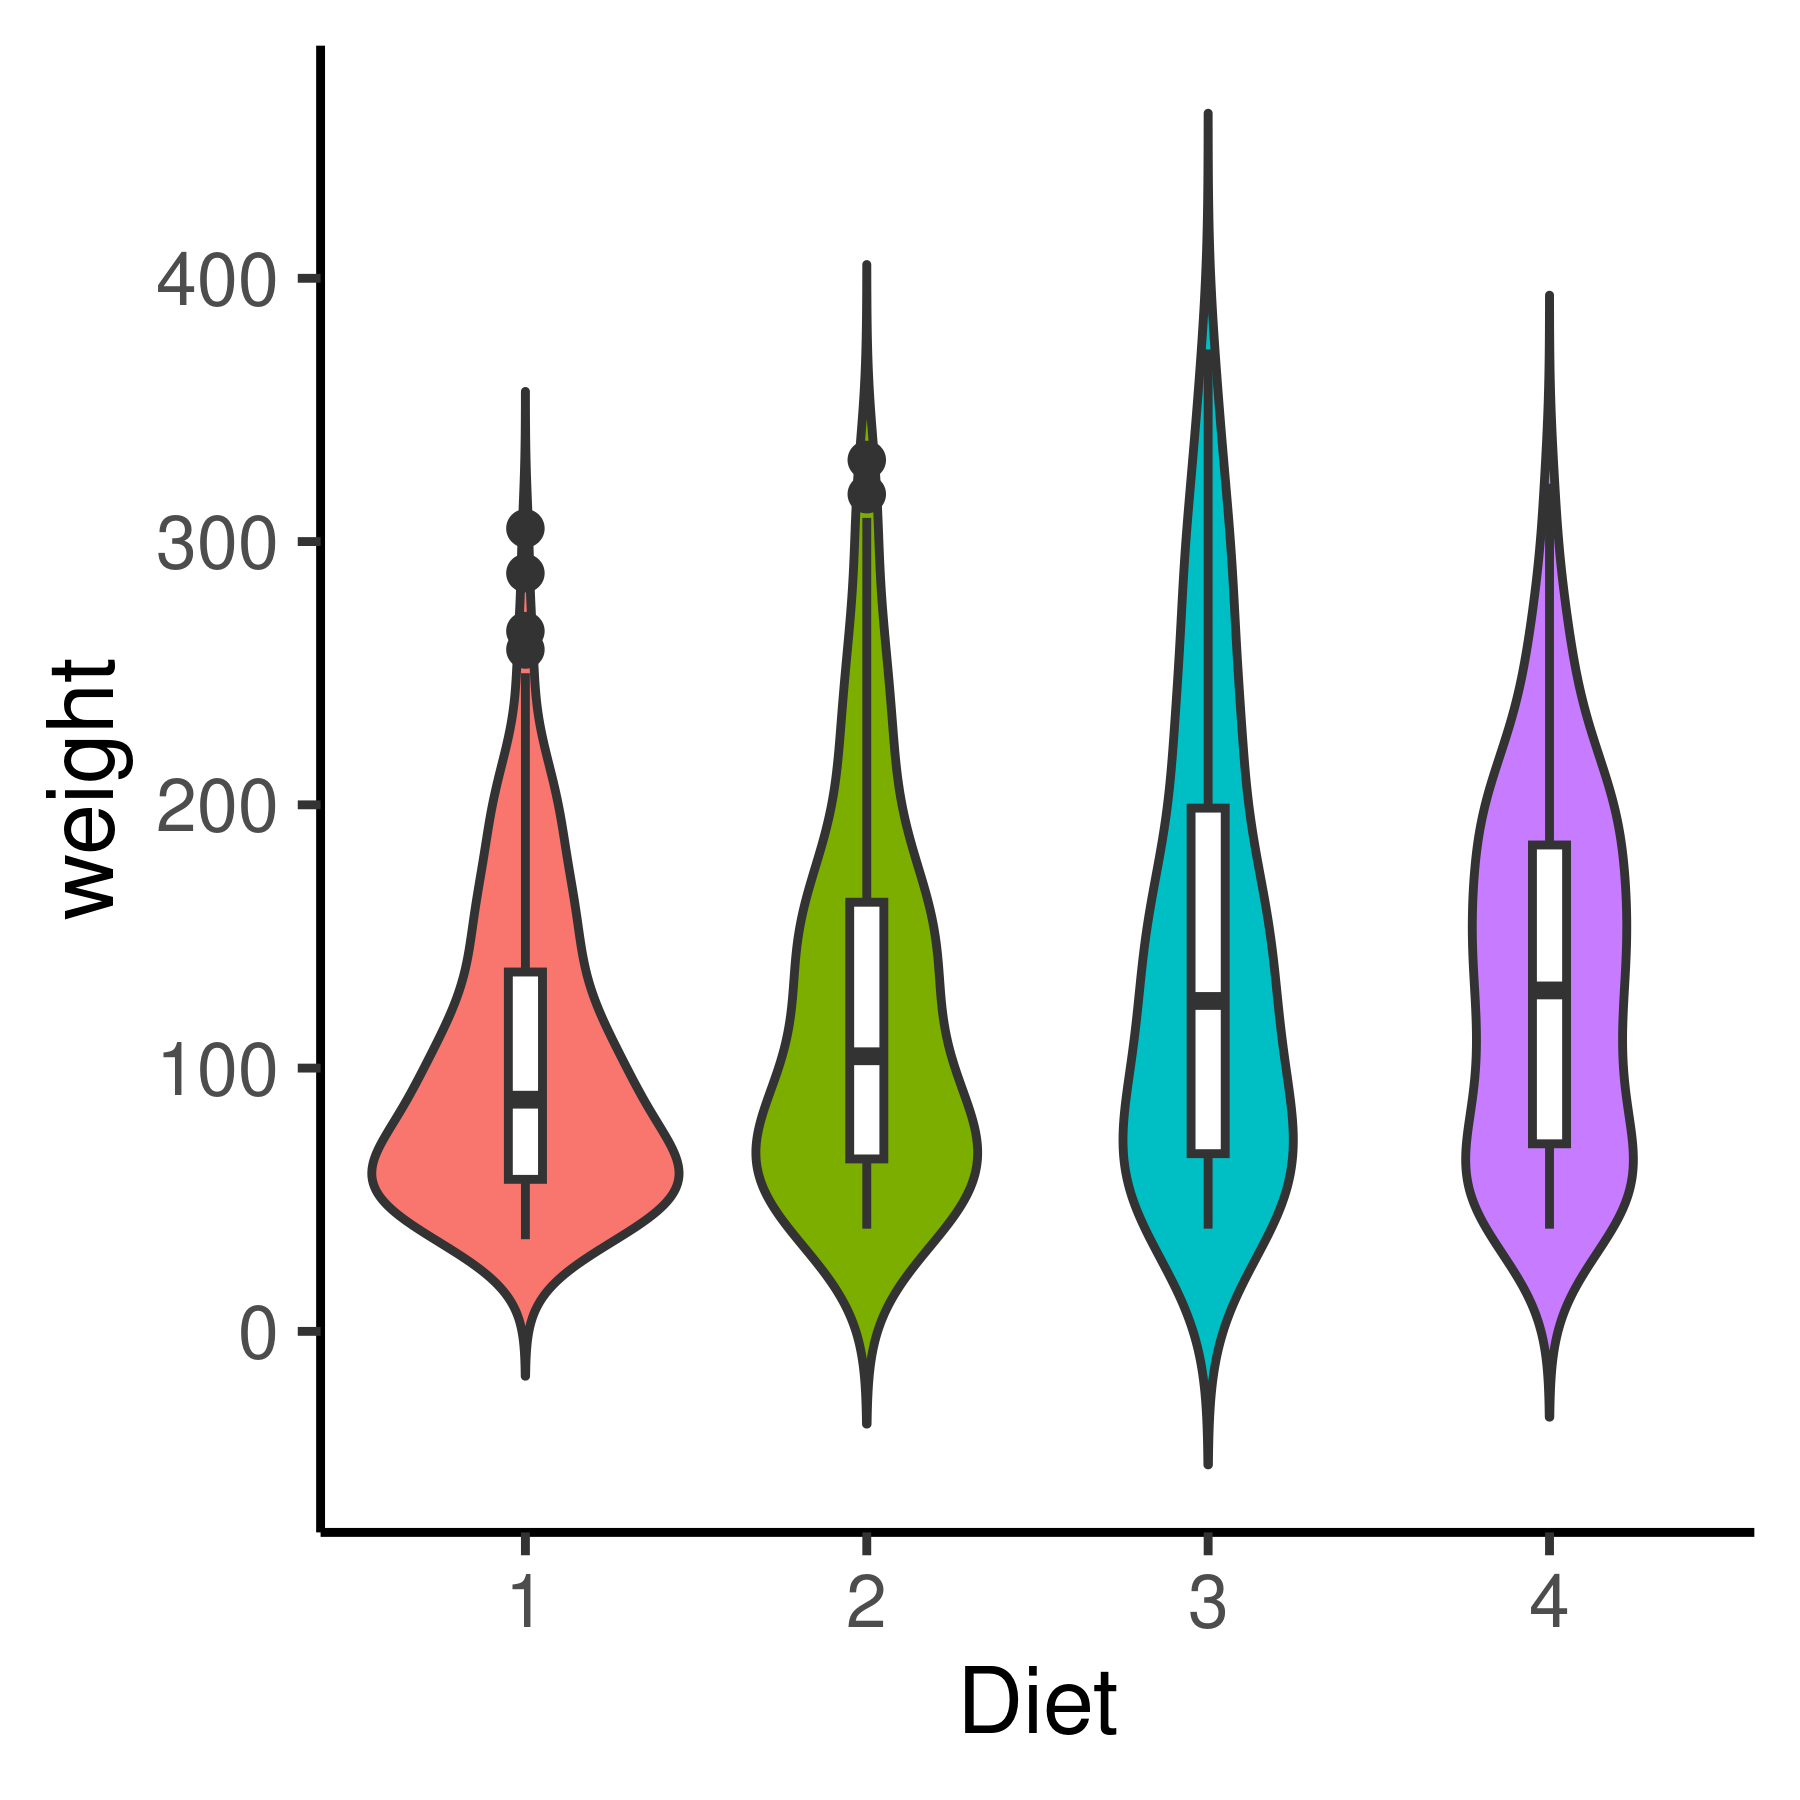
\includegraphics[width=.49\linewidth]{thesis_files/figure-latex/violin_plot1-1} \end{center}

\begin{center}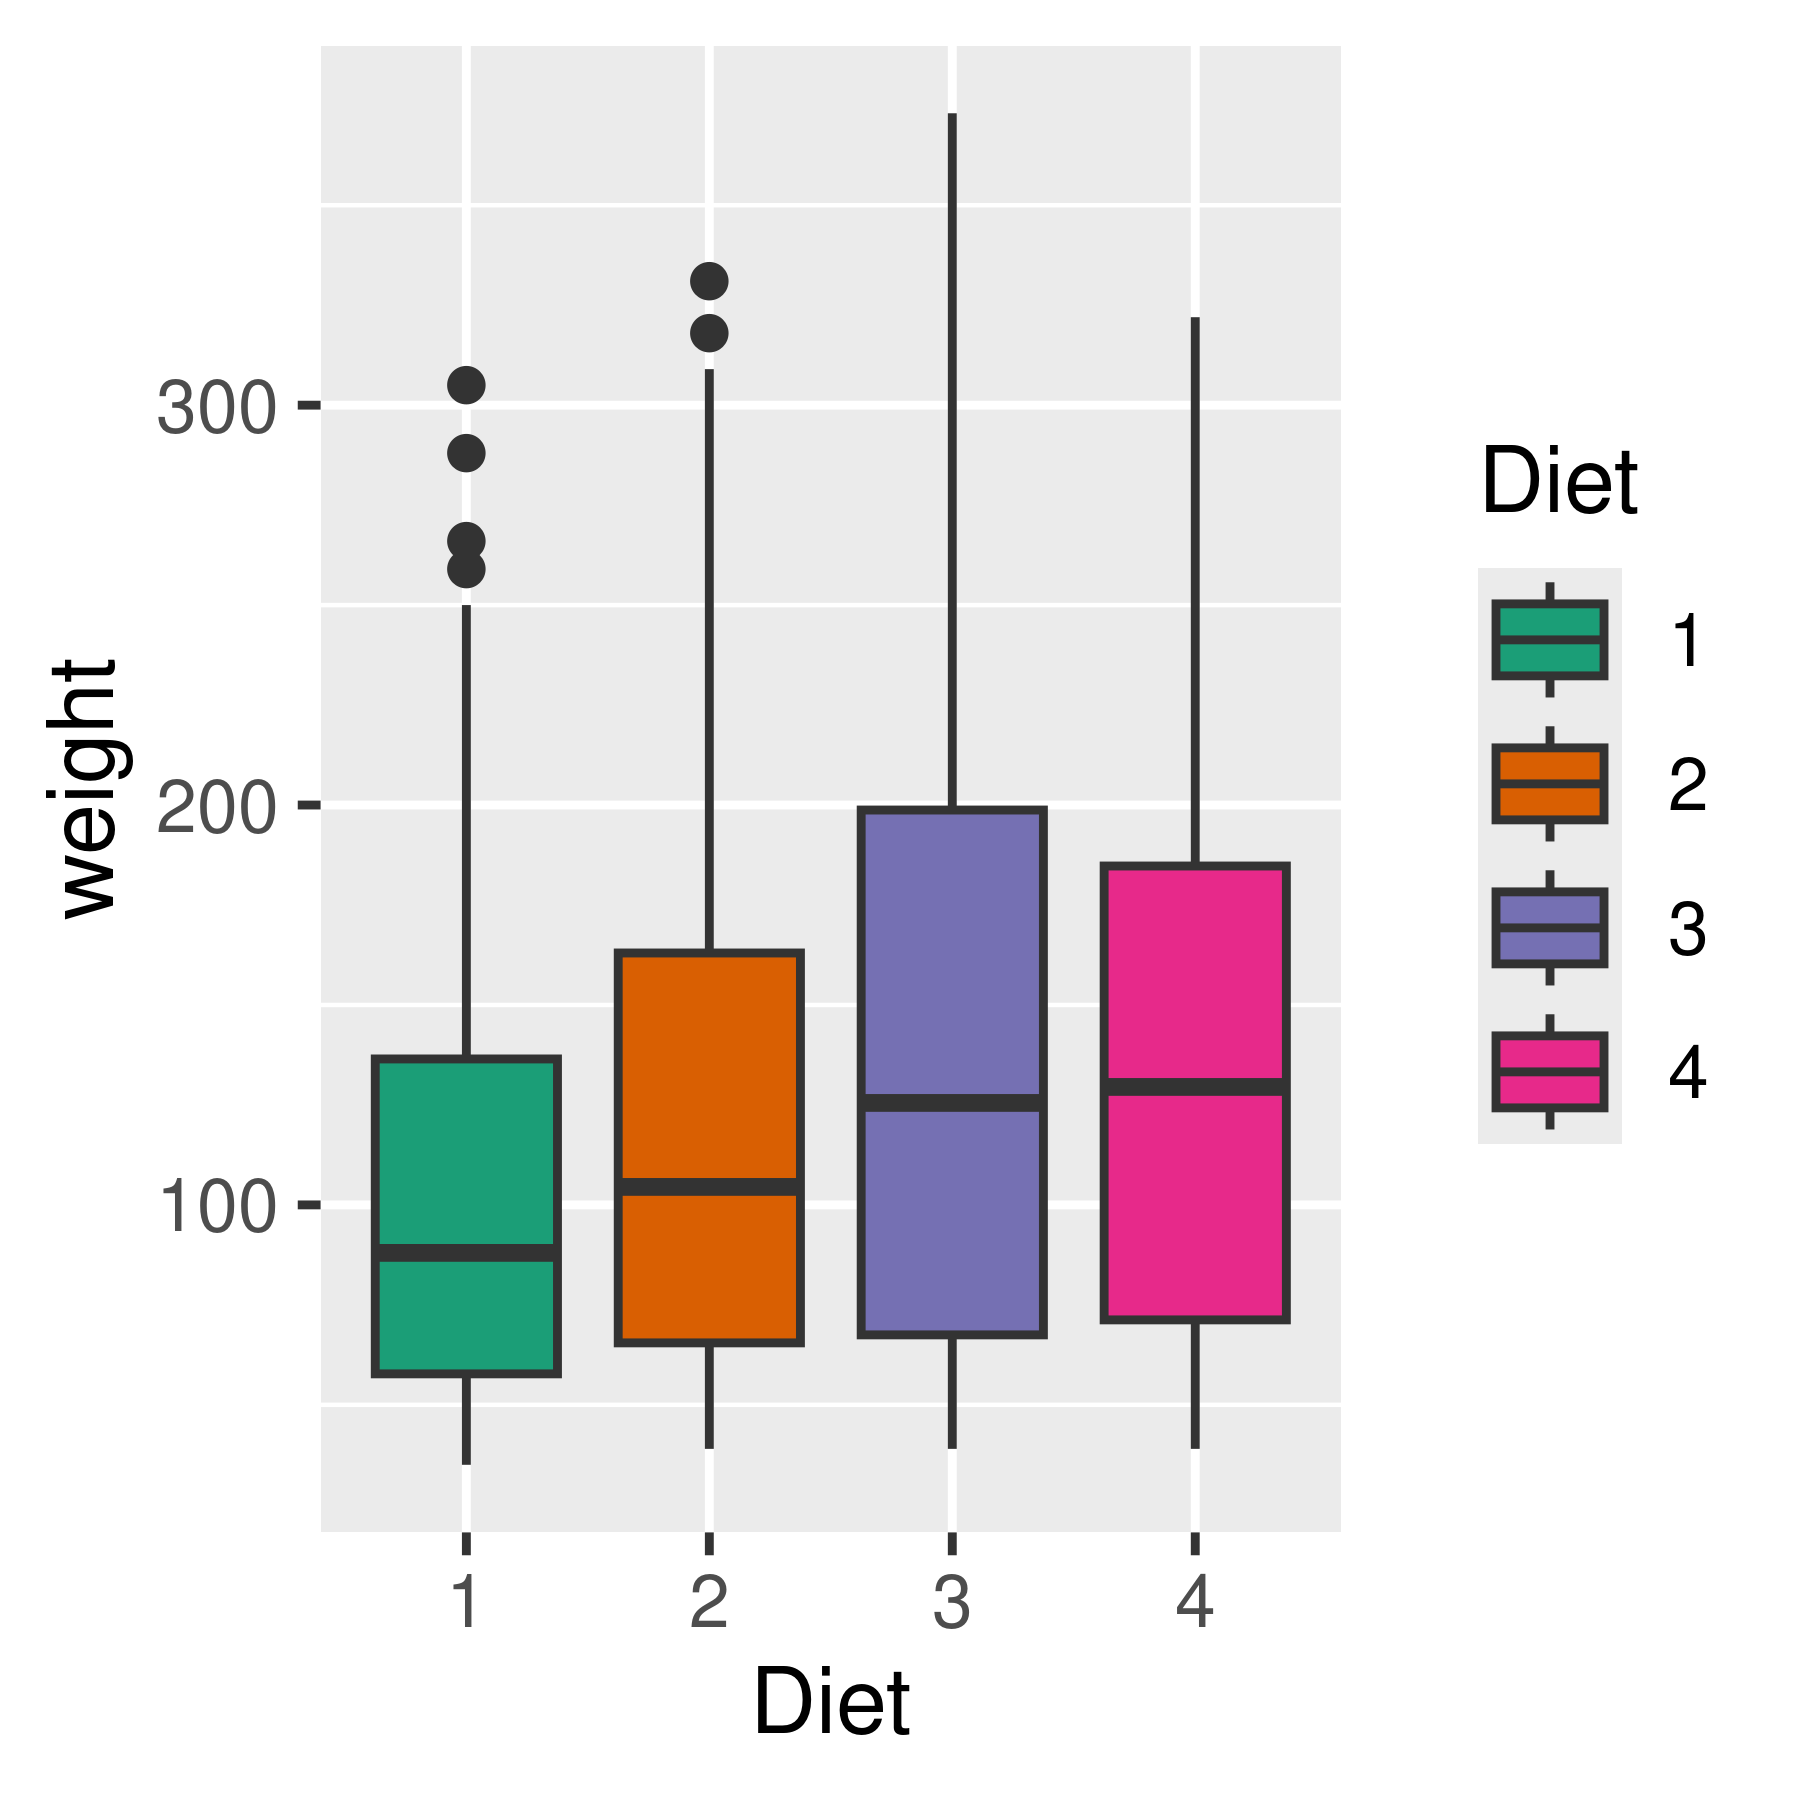
\includegraphics[width=.49\linewidth]{thesis_files/figure-latex/violin_plot1-2} \end{center}

\hypertarget{parallel-coordinate-plots}{%
\section{Parallel Coordinate Plots}\label{parallel-coordinate-plots}}

Parallel coordinate plots (PCPs) are a good way to show data with a lot of dimensions, since each dimension is shown on its own plane.
This means that complex relationships between different factors can be studied over and over again.
PCPs are great for drawing attention to trends, clusters, and outliers, and they know how to use space well to show many aspects in a small area.
But because they overplot, they can get messy with large datasets.
It can be tougher to understand the data than with Cartesian coordinates, and you must go through a learning process to get the the majority of them as well.

Cartesian coordinates, on the other hand, are straightforward to understand because they are simple and well-known.
They make it easier to tell the difference between different information points and their exact values by displaying data points in an easily understood manner.
Cartesian coordinates are an excellent method to present data in a clear way because they can handle up to three dimensions.
They also have trouble with growth because adding more dimensions requires a lot of subplots or complicated three-dimensional plots, which can get boring and challenging to follow.
Cartesian graphs additionally have the ability to take up a lot of room, and for data with more dimensions, they usually need more than one plot.

If you compare PCPs to Cartesian coordinates, PCPs are a powerful way to see and analyze high-dimensional data.
However, they can cause visual clutter and require more practice to understand.
On the other hand, Cartesian coordinates are easy to understand and use for low-dimensional data but can't be scaled up or down for higher dimensions.
The data points are shown as polylines that cross the axes where their coordinate values in each part are equal (Inselberg, 1985).
Traditional parallel coordinate plots (PCPs) have helped show multidimensional data, but when the information gets more significant, they become cluttered and hard to understand.
Other versions of PCPs have been implemented in the theory to enhance the visualization and interpretation of multi-dimensional data, addressing issues such as overlap, scaling, and interaction.

In the article ``Parallel Coordinate and Parallel Coordinate Density Plots,'' Rida E. Moustafa explains a new way to see high-dimensional data using parallel coordinate plots (PCPs) and parallel coordinate density plots (PCDPs).
The primary objective of this work is to make PCPs easier to understand and use since they usually need help with too much mapping and clutter when working with big datasets.
As part of Moustafa's methodology, the standard PCP is mutated into a density plot.
This creates plot areas with more observations that stand out and reduce visual clutter.

The new approach uses density estimation methods to transform the PCP image based on polylines into a continuous, smooth depiction of data density.
This change shows how to see groups and trends usually hidden in regular PCPs.
To make things even better, Moustafa has interactive parts that let users experience different data dimensions in real time.
This makes PCPs even better at analysis. With its interactive nature, people who aren't experts can use this method confidently and successfully.

Moustafa's research indicates that to deal with even larger datasets more efficiently, future efforts should focus on enhancing density estimation methods.
These methods can be used in biology and finance to demonstrate their usefulness and adaptability for examining real-world data (Moustafa, 2011).

The article ``Orientation-Enhanced Parallel Coordinate Plots'' by Raidou et al.~describes a new way to make parallel coordinate plots (PCPs) more accessible to read and understand.
The authors suggest a method that uses input about direction to solve the clutter and overlap problems with regular PCPs.
This method changes the direction of the plot axes on the fly by applying both automatic orientation and user-interactive adjustments.
This method reduces visual noise and makes data patterns and correlations more visible.
This will make it easier for users to study and analyze large datasets.

The suggested orientation-enhanced PCPs are designed with the user's needs at the forefront, offering a more informative visual representation.
Several preprocessing steps, including principal component analysis (PCA) and multi-dimensional scaling (MDS), were employed to determine the optimal axis orientation.
This ensures that data clusters are maximally separated and data lines are minimally overlapped.
The interactive features allow users to adjust the orientation according to their preferences and requirements, enhancing the usability and adaptability of the plots for research needs (Raidou et al., 2015).

The Generalized Parallel Coordinate Plot (GPCP) is an enhancement of the original PCP that adds nonlinear axis changes.
These can show more complicated relationships in the data that might not be visible in a regular PCP.
Nonlinear scales such as logarithmic and exponential transformations are possible.
The 1997 publication ``Visualizing High-Dimensional Structures by Generalized Parallel Coordinate Plots'' by Edward Wegman and Qiang Luo provided a comprehensive discussion of the GPCP idea.
This adjustment allows the visualization to display various data connections and handle skewed data distributions.
It is important to make decisions when resources are limited, and these advanced visual tools make it easier to see how different data sets are related.
As VanderPlas et al.~(2023) show, the basic ideas put forward by Inselberg (1985) are used to build on the rules of today's graphic grammar.

\hypertarget{missing-data-analysis}{%
\section{Missing Data Analysis}\label{missing-data-analysis}}

There have been efforts to understand and deal with missing data.
Cheng et al.~(2015) made a graphical user interface for exploring missing values in multivariable data, and Josse and Husson (2016) created the \texttt{missMDA} package to handle missing values in multivariate analysis.
Since dataset incompleteness directly affects the truth of any later studies, these tools make it clear how important it is to use advanced methods to analyze and deal with it.
These methods are tailored to preserve the multidimensional relationships inherent in GPCP.

There are still issues with handling and displaying missing data in large, difficult datasets, even with the current tools and techniques.
Research has shown several approaches to handling and displaying missing data.
However, there is still a big hole in combining these methods into one system that works for all kinds of data and is easy for people to use.
Unwin et al.~showed MANET, a system that made datasets with missing values accessible through images.
Statistically speaking, lost data needs to be dealt with more complexly with even more advanced tools.
Nevertheless, the tidy data structure must be discussed in more detail.

Stef van Buuren's additional research on missing data created the \texttt{mice} package in R, which is widely used for multiple imputation.
It shows how missing data imputation methods can be used in real life, but at first, they didn't directly connect with the tidy data principles.
This gap highlights the need for a systematic strategy that combines tidy data principles with techniques for managing missing data
As a result, Tierney and Cook developed these principles to address this requirement directly.

Tierney and Cook's 2018 research expands on the principles of tidy data to create an innovative way to deal with missing data.
This method, which describes the role of missing values in data analysis and visualization, represents a major advancement in the discipline.
The paper presents valuable tools for evaluating different interpolation approaches.
These tools are critical for understanding the influence of missing data on research and the many types of imputations that may be used.
Additionally, the study offers tools that can be utilized to compare various estimation methodologies.
Because these tools are intrinsic to the R environment, you can utilize R's statistical capabilities to investigate many types of data loss.
Tools are available to help with missing data visualization, comparing imputation and non-imputed data distributions, and learning how various imputation processes impact statistical results.
Researchers will find this compilation helpful since it explains how to select the most appropriate interpolation algorithms for their data and study.

Newcomers to statistics or researchers with little to no R knowledge may need help with the approaches and code.
The dependence on R as the primary program makes the proposed approaches less accessible to those who use other statistical tools, perhaps restricting their use.

There are several opportunities for expanding their findings.
The key method for making the methodologies more accessible is to include support for other widely used data science tools in the toolkit, such as Python.
A more practical use for these tools would be an automated tool that scores and assesses various estimating algorithms using user-defined criteria.
Finally, clear instructions and examples would be useful for individuals unfamiliar with complicated data imputation techniques and tidy data architecture.

As datasets become larger and more complex, especially in fields that require visualizing high-dimensional data like genomics or big data analytics, current methods often struggle to handle the increased scale or lack the necessary flexibility to effectively address different ways in which data can be missing (Swayne \& Buja, 1998; Schafer \& Graham, 2002).
In academic study, the current state of big data analytics is centered around effectively managing large volumes, wide diversity, and fast data pace.
This poses distinct difficulties in different sectors, such as healthcare and industrial processing.
Significantly, these industries increasingly depend on advanced machine-learning methods to enhance results and prediction capacities.
Integrating big data with artificial intelligence in healthcare improves the capacity to forecast disease trends and treatment results by utilizing extensive data from various sources.
Big data analytics is vital in predictive maintenance and optimizing production processes in industrial environments.
Recent academic reviews emphasize that the future of big data analytics relies on advancing data processing technologies and ensuring their accessibility and effectiveness across various domains.
This underscores the importance of ongoing interdisciplinary research and collaboration to overcome existing barriers and unlock new opportunities (Sabharawal \& Micah, 2021; Rhaul et al., 2023).

Another common approach to present various data types is in parallel coordinates, discussed in the article ``Where Did My Lines Go?''Visualizing Missing Data in Parallel Coordinates'' by Alex Bäuerle et al.~
It is hard to see trends when data is missing because it breaks up the flow of lines. Getting rid of imputations, common ways to deal with missing data, can mess up visual presentations. Based imputation is one of many visualization methods suggested by the authors.
It keeps the general structure and doesn't lead to wrong conclusions.
Some others are dashing, imputation representation with visual cues, and transparency. Real-life studies with users showed that the best ways to find trends were to be open and dash.
The authors also made a tool that lets you use these ways to explore data more interactively. Thanks to their work, we can see incomplete information in a way that is easy to understand.
This is helpful because it avoids adding bias through estimation.
The future work includes making these methods work better with bigger datasets, mixing them with more advanced imputation techniques, and looking into how they can be used in specific fields to make them more reliable and effective (Bäuerle et al., 2022).

Addressing missing data is an analytical challenge in statistical analysis, as incomplete data can lead to biased or misleading results. These methodologies enhance data analysis and decision-making processes.
This dissertation examines advanced techniques for handling missing data, drawing from robust methodologies discussed in recent literature such as Cheng, Cook, and Hofmann (2015) and Tierney and Cook (2018).

These foundational ideas laid the groundwork for contemporary methods of handling missing data in statistical graphics, which are fundamental for providing accurate and meaningful visual interpretations of datasets.

\hypertarget{anomaly-detection-outlier-detection}{%
\section{Anomaly Detection (Outlier Detection)}\label{anomaly-detection-outlier-detection}}

In EDA, treating missing data is not merely a preliminary step but a critical anomaly detection component.
Recognizing patterns of missingness can be a powerful anomaly detection technique, as certain types of missing data may indicate underlying problems or anomalies within the dataset (Rubin, 1976).
Transitioning into anomaly detection, it becomes evident that these missing data patterns can reveal deviations from expected behavior, helping to flag data quality issues or potential outliers that warrant closer examination (Hawkins, 1980).
Thus, the systematic handling and analysis of missing data directly enrich detecting anomalies, underscoring its dual role in EDA.

Wilkinson's ``The Grammar of Graphics'' (2005) is a foundational framework for designing insightful data visualizations integral to EDA.
In this framework, treating missing data is not merely a preliminary step but a key aspect of the analytical process.
Techniques for handling missing data, such as predictive mean matching or multiple imputation, are useful for maintaining the integrity and representativeness of visualizations, allowing for more accurate interpretations and conclusions (van Buuren, 2012).

Furthermore, missing data itself can be indicative of underlying anomalies.
Analyzing patterns of missingness can reveal data integrity issues, systematic errors, or anomalies in data collection processes, which are often critical for domains like clinical trials or quality control in manufacturing (Little \& Rubin, 2002).
Once a dataset has been adjusted for missing values, visual techniques---such as enhanced scatterplots or layered density plots---can effectively detect outliers and unusual patterns.
These visualizations are pivotal in fraud detection or environmental monitoring, where quick identification of deviations from expected patterns can lead to prompt and necessary actions (Unwin et al., 2006).

Thus, handling missing data effectively enriches the dataset, enabling more robust anomaly detection through sophisticated visual tools.
This ensures that the visualizations represent the observed data and highlight the absence of data as potential markers of critical anomalies, thereby supporting deeper and more comprehensive analytical insights.

Both reducing the value of anomalies and eliminating them are primary goals of anomaly detection along with identifying their underlying cause.
Walter A. Shewhart's research on statistical control mechanisms in the 1920s is the ancestor of anomaly identification in statistical graphics.
Statistical process control (SPC) was made possible by Shewhart's creation of the control chart, an important tool for finding problems in the manufacturing process (Shewhart, 1931). Examine the picture below.
In addition, MSPC charts are an expansion of univariate statistical process control approaches that are used to track the efficiency of processes with numerous interconnected variables.
It was Hotelling's 1947 introduction of the multivariate control chart that laid the groundwork for MSPC.
According to Hotelling (1947), this was a huge improvement over the previous generation of charts, known as univariate Shewhart charts, which were limited to handling variables individually.
Many thanks to Jackson (1980) for using PCA to track multiple variables and Nomikos and MacGregor (1990) for their work on multivariate SPC charts using PCA and PLS, which made the foundations of MSPC even stronger (Jackson, 1980; Nomikos \& MacGregor, 1995).

When software and computers came out in the middle of the 20th century, they transformed how things worked in the field.
John Tukey's exploratory data analysis work introduced basic graphing methods for finding outliers and other strange things in data.
His methods, such as box and scatter plots, were particularly efficient at finding variations between sets of data (Tukey, 1977). Shewhart's SPC charts were essential to improving and keeping quality under control.
They show the difference between general and special cause deviations in industrial processes.
Tukey also uses statistical techniques to find trends, outliers, and inconsistencies in the data when completing statistical analysis. This demonstrates his appreciation for understanding the dynamic nature of data.
Both Shewhart and Tukey supported the use of visual tools to discover insights in data.
One way to visually observe the stability and control of a process is with Shewhart's control charts.
Tukey also developed a number of plotting methods to aid analysts in making sense of data, such as the box plot and the stem-and-leaf plot.
The fact that they are connected shows how strongly they believe in the capacity of visual data analysis to help find patterns and make better decisions.

Anomalies in multivariate data sets can be effectively illustrated using generalized parallel coordinate plots (GPCPs), which expand the traditional capabilities of parallel coordinate plots to include both continuous and categorical variables.
A strategy for handling complications caused by neighboring category variables is described by Vanderplas et al.~(2023) as ``factor blocks.''
A categorical variable's combined distribution with other categorical variables determines its ordering inside each level in these charts.
In more conventional arrangements, this serves to lessen the visual noise that could mask important patterns.
By graphically organizing the data, this method not only helps to spot outliers but also draws attention to key relationships within the data.

By manipulating the order of line plots, a ``layered approach'' to high-dimensional data management optimizes overplotting control.
This approach makes it easier for the user to follow specific observations across the graph, even when there is a lot of data.
An effective tool for anomaly identification is thus created by combining those methods within GPCPs. This tool successfully manages and represents the complexity that is built into multivariate datasets.

It is vital to discern anomalies indicating significant insights or errors in GPCP.

In ``Novelty Detection: A Review---Part 1: Statistical Approaches,'' Markou and Singh (2003) provide an in-depth review of the various real-world applications that utilize novelty detection techniques.
The authors conduct extensive research in these areas to understand better the pros and cons of parametric, non-parametric, and semi-parametric statistical analytic methodologies.
To improve recognition and make the system more adaptable, they suggest that researchers should combine statistical methodologies with machine learning strategies in the future.
Modern applications are becoming more dependent on data with complex structures and many properties.
This emphasizes the significance of establishing better and more reliable methods for handling this information.
This new direction has significance for the advancement of the field and for scientists to tackle the ever-evolving challenges of detecting new patterns in diverse datasets.

In their 2009 article ``Fast Detection and Visualization of Network Attacks on Parallel Coordinates,'' Choi, Lee, and Kim propose a technique for seeing and recognizing network attacks in a moment using parallel coordinates.
The complex multivariate data interactions can be better understood with the assistance of this tool.
This study demonstrates how to use parallel coordinates to show various network data dimensions simultaneously, which helps spot unusual trends that can indicate security breaches immediately.
For future work, the authors suggest investigating how to add real-time data processing techniques to their system to improve it and make it more effective in finding things.
Their recommendation to enhance the system's usability and efficiency in a real-world security operation center scenario involves strengthening its data visualization features to manage larger datasets better.
This future path is necessary to build increasingly sophisticated, real-time security monitoring systems that can handle the growing number and sophistication of network dangers.

Pimentel et al.~(2014) explore the subject matter of novelty detection in their comprehensive review titled ``A Review of Novelty Detection.''
Novelty detection is essential when discovering novel and unique data patterns deviating significantly from established standards.
The study uses machine learning models like neural networks and support vector machines and statistical methods such as nearest-neighbor and grouping techniques.
Pimentel et al.~emphasize the need for future research to create hybrid models incorporating several detection approaches to enhance accuracy and robustness.
Future research should prioritize scalability and the capacity to adjust to new patterns and changing surroundings quickly.
They further recommend improved approaches to managing streaming data in systems that operate in real-time.

Research by Ding et al., published in 2014 as ``An Experimental Evaluation of Novelty Detection Methods,'' compares and contrasts different approaches for detecting novelty and evaluates how well they perform in diverse data scenarios.
Evaluations of statistical, machine learning and hybrid approaches are carried out with the support of several baseline datasets.
According to the outcomes, each strategy offers benefits and drawbacks.
The writers explain in detail how these algorithms handle various forms of data noise and how various realistic parameter changes affect how well they perform.
In addition, Ding et al.~say that domain-specific data should be added to novelty recognition systems to make them easier to understand and work better.
As a result, this is of paramount importance in certain sectors, such as healthcare and finance, where specialized approaches are required.

Enhanced statistical summaries can be achieved by expanding the grammar of graphics, as discussed in Hadley Wickham's ``A Layered Grammar of Graphics'' (Wickham, 2010, Journal of Computational and Graphical Statistics).
Wickham suggests adding layers to the grammar of graphics in order to separate statistical reports and visualizations can be stacked on top of one another.
This technique can be very helpful in discovering novel ideas because it helps you add normal data representations with accents or different styles for data points that are distinctive novel or different.
This layered technique makes it less difficult to see the difference between standard and unusual data.
It might be interesting to look into how to generate the layers based on statistical significance or anomaly scores.
Machine learning methods could be used to create the visualization layers and change as new data is processed.
A further area that could be focused on is making interactive visualization tools that let users change the elements that determine what is new and see immediately how these changes affect the output graphics.

``Anomaly Detection in Streaming Nonstationary Temporal Data'' by Pasha et al.~(2017, Journal of Machine Learning Research) examines methods to identify problems in streams of temporal data.
It does this by using visualization techniques that are compatible with the grammar of graphics to demonstrate issues in real-time.
The authors suggest a framework that may adapt according to changes in the statistical properties of the data.
This makes sense for purposes like network security or monitoring sensor data in real-time.
Visualizations are very important here, given that they provide you immediate feedback on identifying any potential issues.
Introducing user feedback loops to the system might make the detection algorithms adaptable by giving them the ability to shift their rules based on what users think about false positives and missed detections.

Current research primarily addresses either data visualization or anomaly detection independently, with insufficient focus on their interaction (Alvarez \& Oliva, 2009; Choi et al., 2009).

In their interesting 2011 research paper ``Evaluation of Parallel Coordinates for Interactive Alarm Filtering,'' Azhar and Rissanen examine the possible benefits of using parallel coordinates to filter and evaluate alerts in complex systems.
The study examines the ease of use of the interface and how well this visual style improves the quick recognition of important patterns and alarms.
The authors come to the conclusion that parallel coordinates may improve the alarm filtering process more effectively but likewise point out ways in which it may be made better in the future.
They state that the interface should be changed to ensure it facilitates faster cognitive thinking and makes users less fatigued.
By testing the interface in more types of real-world settings, we could discover more about how helpful and efficient it is in a range of disciplines and systems.
This could help make the tool better fit the requirements of different groups of users.

In ``Information-theoretic outlier detection for large-scale categorical data,'' Wu and Wang (2013) introduce an information-theoretic approach to identify outliers in datasets with categorical variables.
The method leverages entropy measurements to quantify the degree of abnormality in the data, thus providing a robust framework for detecting deviations from expected patterns.
This approach is particularly effective in handling large-scale datasets where traditional statistical methods may shall.
The authors identify several avenues for future work, including enhancing computational efficiency for even larger datasets and integrating this approach with other data types, such as numerical or mixed datasets.
Further research could also explore the application of this method in specific industry contexts, such as cybersecurity or healthcare, where outlier detection is critical yet challenging due to the categorical nature of much of the data.

In their 2013 article titled ``Information-theoretic outlier detection for large-scale categorical data,'' Wu and Wang explain an approach to finding outliers in datasets with categorical variables using information theory.
The approach uses entropy measurements to figure out how strange the data are, which makes it simple to identify trends that don't match up with what one might expect.
This approach works particularly well with large data sets, where various other statistical techniques may not be successful.
The authors propose a variety of places for further study, such as making computations faster for larger datasets and combining this approach with different types of data, like mixed or numerical datasets.
Further research might also look into how this approach may be used in certain fields, like cybersecurity or healthcare, where identifying outliers is important but tricky given that much of the data is categorical.

The importance of algorithms for identifying anomalies in categorical data is emphasized in fields like fraud detection and network security in ``Anomaly detection methods for categorical data: A review'' by Taha and Hadi.
They dissect methods into five groups: rule-based, logistic, probabilistic, and information theory-based.
Measurement metrics like recall, F-measures, accuracy, precision, and area under the curve (AUC) are discussed, stressing problems related to imbalanced datasets.
The report highlights practical issues by including examples like fraud and disease outbreak detection.
The writers say these problems are scalability, high-dimensional data, and interpretability.
Future research directions aim to expand the anomaly detection field for categorical data, including developing hybrid methods, new evaluation metrics, standard datasets, scalable algorithms, dimensionality reduction techniques, and interpretable models. (Taha \& Hadi, 2019)

In their review, Taha and Hadi classify many approaches to anomaly detection for categorical data, which includes methods based on probabilistic models, distance, information theory, clustering, and rules.

Probabilistic models like Bayesian networks and hidden Markov models make it easy to work with different kinds of data.
These models can also show how factors are related in complex ways. In addition to being masters at managing uncertainty, they provide decision-makers with probabilistic estimates of anomaly scores.
However, these models' computational intensity might increase significantly when dealing with significant or high-dimensional data.
A large quantity of data is frequently necessary to accurately estimate the parameters of probabilistic models.

A simple way to find outliers is to use distance-based methods, like the Hamming distance and similar measures.
These tools are easy to understand and use because they measure how different two sets of data are from each other.
Because category values are ordered, finding an excellent way to measure distance for them can be tricky.
One problem with these methods is that it can take a lot of time and computing power to figure out the lengths between all pairs of data points.

Information theory-based methods use changes in entropy and mutual information to find things that don't seem right.
Many of these methods are data-based and only need a little setting tuning.
It is important to remember, though, that information-theoretic measures can be hard to understand and use and that they don't always work well with noisy data, which can cause false positives.

Clustering methods, like k-modes and conceptual clustering, make it easier to find misfits by naturally grouping similar data points.
They are great for many data sources because they are flexible and can learn from unlabeled data.
Still, it might be hard to find the correct number of clusters if you don't have subject knowledge or heuristics.
Also, grouping methods require a lot of computing power, so ways to use them may need to be more efficient when working with large datasets.

Using rules-based methods is a straightforward way to explain why a data point is abnormal.
These include decision trees and link rules. They are also very flexible and can quickly pick up rule-based subject knowledge.
Still, rule sets can get very big and complex to use as data complexity increases.
Also, overfitting is a possibility.
This happens when the rules are too tightly matched to the training data and need help to handle new data. This is especially true for small datasets.

The literature indicates a lack of robust, scalable methods that can simultaneously visualize and detect novel patterns in mixed-attribute data sets efficiently (Azhar \& Rissanen, 2011; Wu \& Wang, 2013; Taha \& Hadi, 2019; Bäuerle et al., 2022).
This gap underscores the need for a holistic approach that addresses the visualization complexities of mixed attributes and incorporates effective, real-time novelty detection mechanisms to aid in faster and more accurate decision-making processes.

By integrating these approaches into the grammar of graphics packages in R, this research simplifies the diagnostic and remediation processes for missing data, ensuring more accurate and reliable analysis for developing effective data dashboards.

\hypertarget{dimension-reduction}{%
\section{Dimension Reduction}\label{dimension-reduction}}

Exploratory Data Analysis (EDA) and Dimension Reduction Techniques are closely intertwined in the realm of data analysis.
EDA serves as the initial step in understanding and visualizing complex datasets, helping analysts uncover patterns, anomalies, and relationships within the data.
However, as datasets grow in dimensionality, the complexity of EDA can become overwhelming. This is where Dimension Reduction Techniques come into play.
By reducing the number of features or variables while preserving the most critical information, these methods simplify the data, making it more manageable for further analysis.
Dimension Reduction Techniques, such as Principal Component Analysis (PCA) or t-Distributed Stochastic Neighbor Embedding (t-SNE), complement EDA by providing a way to condense high-dimensional data into a lower-dimensional space without losing significant insights.
This synergy between EDA and Dimension Reduction Techniques empowers data scientists and analysts to gain deeper insights into their data while efficiently handling large and complex datasets.

\hypertarget{interactive-graphics}{%
\section{Interactive Graphics}\label{interactive-graphics}}

Interactive graphics are essential to EDA (Unwin, 1999).
Beyond the limitations of static statistical displays, interactive graphics enable visualizations to advance alongside the analysis.
User interaction and direct manipulation are required for dynamic graphics to reach their full potential (Cook, Buja, Cabrera, \& Hurley (1995); Unwin (1999)).
The connection between EDA and dashboards is that EDA is the process of preparing and understanding the data, which is the first step for building a dashboard, as the data has to be cleaned, transformed, and analyzed to be used efficiently on the dashboard.
EDA results can be used to identify the most relevant data and metrics to include in the dashboard and to design the visualizations that will be used to display the data.
Additionally, the EDA process can identify the outliers, patterns, trends, and insights helpful to show in the dashboard to support decision-making.

\hypertarget{rmd-basics}{%
\chapter{Chapter Paper on Rural Shrink Smart Manuscript submitted to Journal of Data Science Special Issue}\label{rmd-basics}}

\hypertarget{abstract}{%
\section{Abstract}\label{abstract}}

Many small and rural places are shrinking. Interactive dashboards are the most common use cases for data visualization and context for exploratory data tools. In our paper, we will explore the specific scope of how dashboards are used in small and rural area to empower novice analysts to make data-driven decisions. Our framework will suggest a number of research directions to better support small and rural places from shrinking using an interactive dashboard design, implementation and use for the every day analyst.

\hypertarget{introduction-1}{%
\section{Introduction}\label{introduction-1}}

As the amount of data has increased in nearly every facet of life, the need to make sense of that data in an approachable, accessible form has become ever more important.
As a result, many companies and organizations use interactive dashboards to present these data in a more useful and visually appealing form (Sarikaya, Correll, Bartram, Tory, \& Fisher, 2019).

In many cases, dashboards support viewers' information processing, helping to make sense of complex data, navigate through a dataset, and supporting decision making based on the data.

Dashboards are often used, as with the car display of the same name, to provide summary information about many separate attributes of a common entity. One glance at a car's dashboard will tell you the speed, RPM, engine temperature, amount of gas in the tank; more importantly, however, the goal is not for the user to remember all of these characteristics, but to assess whether any of these quantities is outside of the expected range.
Similarly, interactive dashboards for data are often used to display many different attributes and performance metrics which are of importance for stakeholders.

In this paper, we discuss the process of designing a dashboard to present publicly available government data to stakeholders in small Iowa towns to facilitate decision making and objective comparison with other similarly-situated towns.

Some communities continue to thrive as they lose population because they adapt, maintaining quality of life and community services for residents while investing in the future. This process, \emph{smart shrinkage}, is important for rural areas who have experienced shrinking populations for decades. As small rural towns do not have access to data scientists or even the ability to easily leverage data collected locally to support decisions, our research team will provide communities with data about services in small town Iowa in order to assist with developing strategies to improve quality of life for their residents amid shrinking populations (Rural Shrink Smart Team, 2022). We hope to allow towns to explore their own data and compare to other similar towns, centering decision-making on data in the context of small-town Iowa life.

\hypertarget{data-description}{%
\section{Data Description}\label{data-description}}

The Smart and Connected Community (SCC) dashboard data are primarily assembled from \url{data.iowa.gov} (State of Iowa, 2020), with some additional datasets assembled from federal and private sources. Most of these data sets are collected at a town/city or county spatial resolution, requiring us to carefully join data to ensure that these differences are respected while collating relevant information at the city level. In addition to the more commonly available statistics derived from e.g.~the census and American Community Survey, \url{data.iowa.gov} contains several unique data sets, including local liquor sales, school building locations, town budgets and expenditures, hospital beds, Medicaid reimbursements, and other details that may provide information about local quality of life.

Data available on Iowa's data portal were augmented in some cases with higher-quality data sets in cases where the Iowa data were out of date or insufficiently accurate.
Data collected from ELSI (National Center for Education Statistics, 2020) from \url{https://nces.ed.gov} were used to show the distance to any private or public school. The National Center for Education Statistics (NCES) is the primary federal entity for collecting and analyzing data related to education (Zarecor, Peters, \& Hamideh, 2021).

Data collected from the Index of Relative Rurality (IRR) (USDA - ERS, 2020a) were used in the SCC dashboard to help classify the towns. The Index of Relative Rurality (IRR) is a continuous, threshold-free, and unit-free measure of rurality. It is an alternative to the traditional discrete threshold-based classifications.The IRR ranges between 0 (low level of rurality, i.e., urban) and 1 (most rural). Four steps are involved in its design:

\begin{enumerate}
\item Identifying the dimensions of rurality: population size, density, remoteness, and built-up area.
\item Selecting measurable variables to adequately represent each dimension:
    \begin{itemize}
        \item Size: logarithm of population size
        \item Density: logarithm of population density.
        \item Remoteness: network distance.
        \item Built-up area: urban area (as defined by the US Census Bureau) as a percentage of total land area.
    \end{itemize}
\item Re-scaling the variables onto bounded scales that range from 0 to 1.
\item Selecting a link function: unweighted average of the four re-scaled variable.
\end{enumerate}

Data collected from Rural Urban Commuting Area Codes (USDA - ERS, 2020b) were used to help identify towns with commuting behaviors in our rural areas. The rural-urban commuting area (RUCA) codes classify U.S. census tracts using measures of population density, urbanization, and daily commuting. This data is on a zip code-level that will help identify those communities that commute to more urban areas. The most recent RUCA codes are based on data from the 2010 decennial census and the 2006-10 American Community Survey. The classification contains two levels. Whole numbers (1-10) delineate metropolitan, micropolitan, small town, and rural commuting areas based on the size and direction of the primary (largest) commuting flows.

One of the interesting features of this assembled data set is that missing data can be missing for multiple reasons: not all state data is complete, but data about certain services may also be missing because towns do not offer that service.
Thus, in addition to the usual challenges of working with real-world data that is ``messy'' in a variety of ways, we also have to contend with missing data that is missing due to the size of the community or the lack of services. This makes both visualization and statistical analysis more complicated (and more interesting).

\hypertarget{dashboard-design-considerations}{%
\section{Dashboard Design Considerations}\label{dashboard-design-considerations}}

\begin{figure}
\hypertarget{fig:metrics}{%
\centering
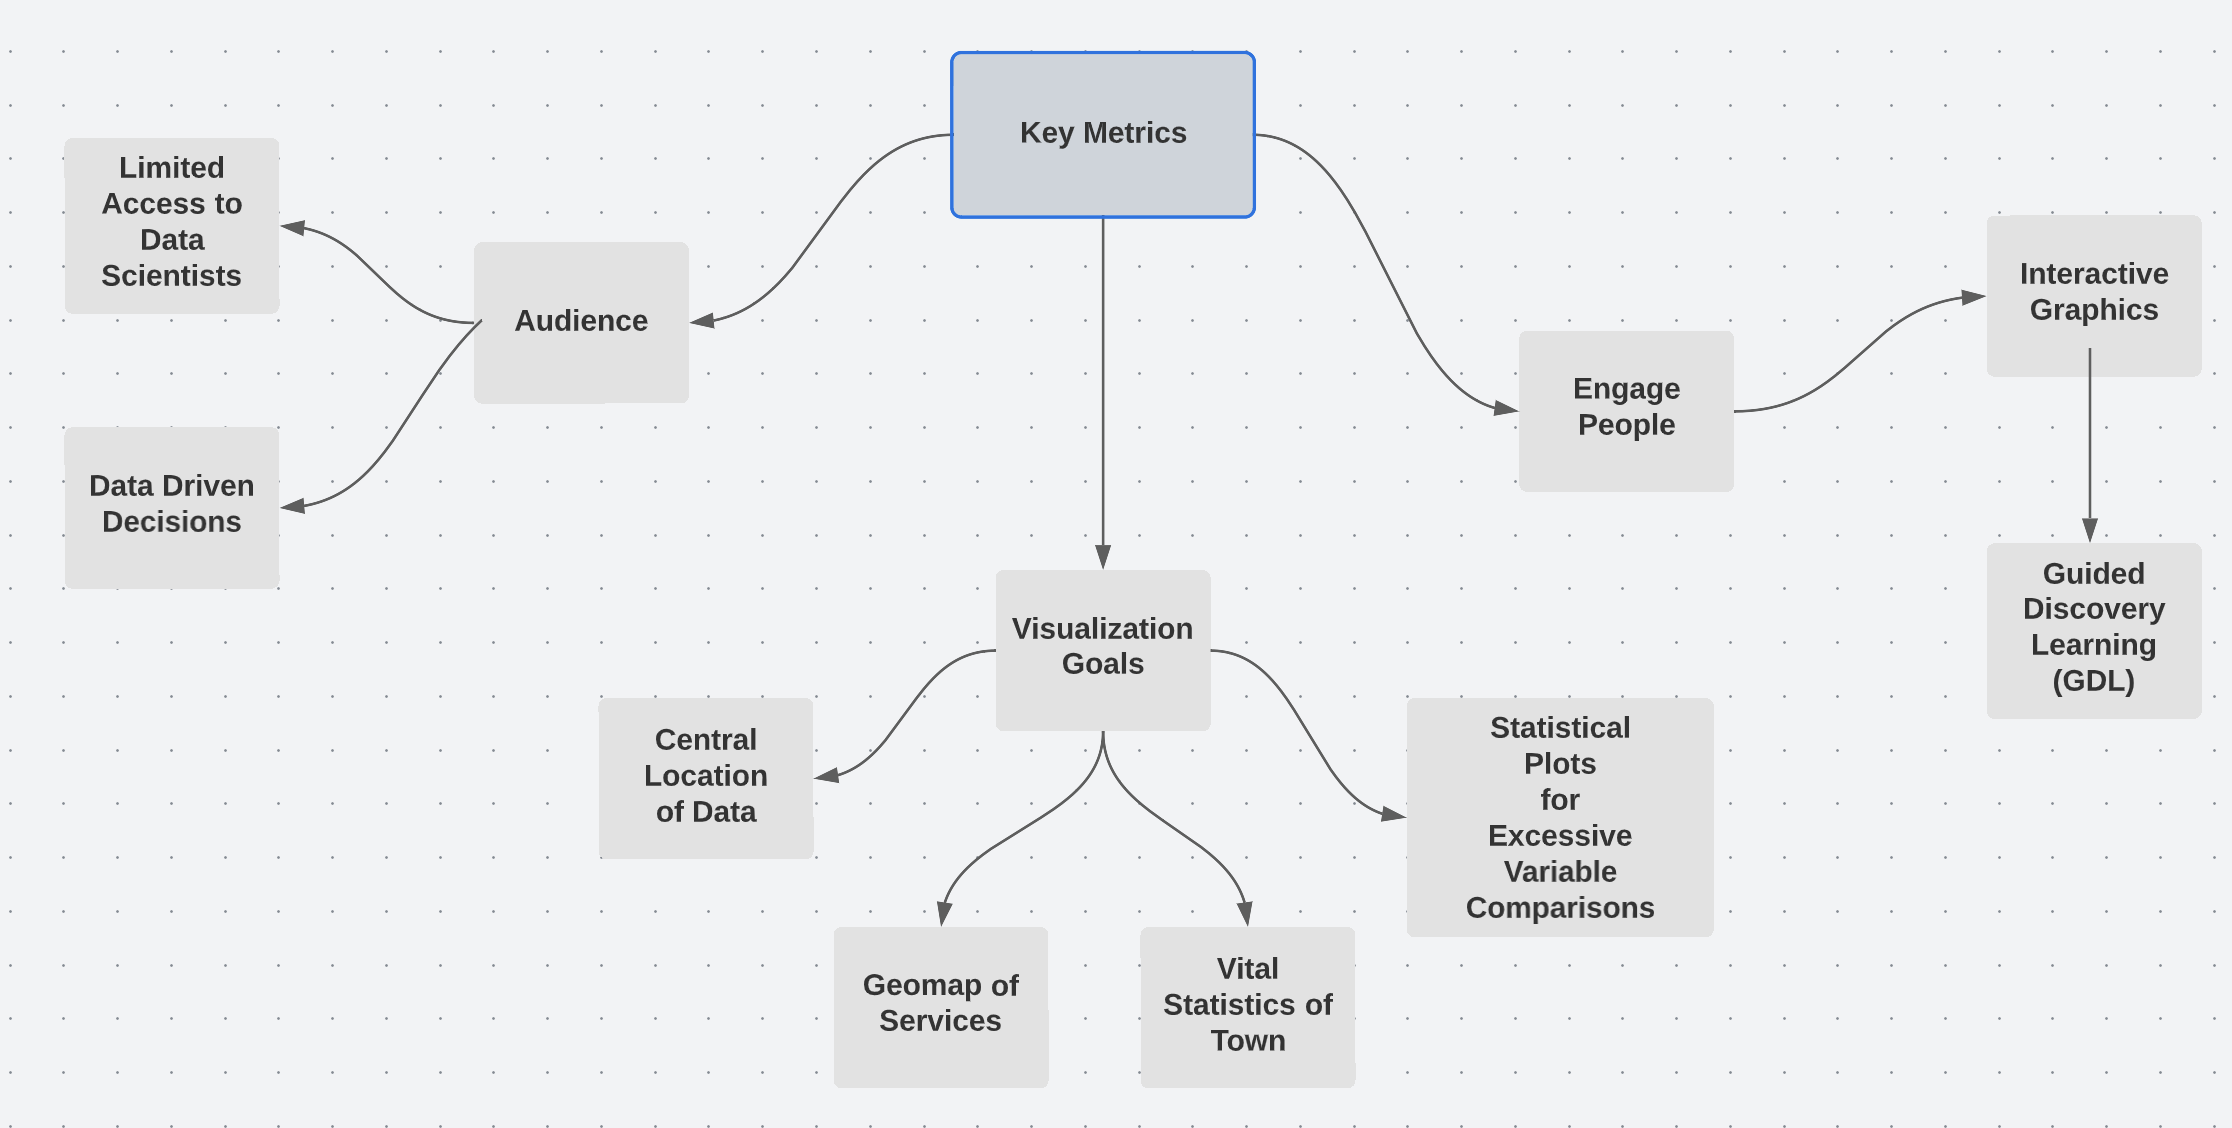
\includegraphics{figure/KeyMetrics.png}
\caption{Diagram of considerations for our dashboard design process.}\label{fig:metrics}
}
\end{figure}

One problem we identified early in the process of assessing smart-shrinkage strategies in small towns is that these towns do not have the resources to make data-driven decisions. Typically, small towns in Iowa are managed by at most a few part-time employees or volunteers. In some cases, essential management functions of the town are paid, but the municipalities we are interested in do not have sufficient funding to hire professionals to gather and analyze data.

As part of a wider project investigating the strategies towns use to maintain quality of life amid shrinking population, our research team provides communities with data about their own town, but also comparable towns across the state which may have a different approach to city services. In combination with other engagement strategies that are more qualitative, we hope to use this interactive dashboard approach to assist small Iowa cities with generalizing and developing strategies to improve or maintain quality of life amid shrinking populations.

One factor at the forefront of our visualization design is the importance of reducing the cognitive demands on viewers: we have assembled an incredible amount of data, and it is easy for even statisticians who deal with much larger datasets to get lost in the details of this data. At the same time, we want to invite viewers to engage with the data - to imagine, to draw comparisons, to generalize across towns, and to integrate outside information into the conclusions drawn based on the data we present.
This invitation to engage with the data is similar to the approach advocated in Guided Discovery Learning, a framework leverages hints, feedback, and other helpful information to guide users in interactive exploration (DeDonno, 2016).

We expect that users will be interested in ``sets'' of variables from the wider dataset, which we assembled based on quality of life factors in the Iowa Small Town Poll (Peters, 2019). For instance, users might be interested in medical and social services available to residents, such as a local primary care clinic, nursing homes which are within driving distance, and the distance to the nearest emergency room; these factors might be explored separately from variables describing the services provided directly by city government, such as parks and recreation expenditures, snow removal services, and the distance to the closest fire station.

As a consequence of this massively multivariate structure, we very quickly focused on the use of parallel coordinate plots; other alternatives, such as tours (Wickham, Cook, Hofmann, \& Buja, 2011), require much more sustained attention to interactive plots as well as a deeper understanding of projections in multidimensional space which we cannot assume our users will have. Introduced in the 1880s (d'Ocagne, 1885), parallel coordinate or parallel set plots feature a series of vertical axes representing different variables arranged horizontally, with lines connecting each observation. When representing categorical data, parallel set plots may show ``blocks'' of data instead of individual lines, and are useful for representing conditional relationships between adjacent variables (Bendix, Kosara, \& Hauser, 2005); modifications of this design, such as common-angle plots (Hofmann \& Vendettuoli, 2013), address the issues which arise due to line-width illusions VanderPlas \& Hofmann (2015a). Parallel coordinate plots have been generalized to allow for continuous data and additional summaries beyond individual data points, such as densities (Heinrich \& Weiskopf, 2009). In this paper, we use the \texttt{ggpcp} package, which leverages the grammar-of-graphics framework introduced in Wickham (2016), allowing us to use not only parallel coordinate plots, but also to overlay other statistical summaries, such as boxplots or violin plots, to provide additional context about the marginal distributions of each variable in addition to allowing for exploration of the multivariate space.

We also anticipate that users will be interested in comparing their town to other, similar towns. We will discuss the different ways that this comparison strategy was implemented in each dashboard in the next section, which describes the evolution of the dashboard over time and accounting for feedback from users and other researchers on the wider project.

One final component of this project is that our dashboard is part of a wider effort to work with towns to understand the different strategies used to maintain resident quality of life amid shrinking populations. Thus, while the town leaders are our primary audience, we also are creating this applet for use in parallel with a team of other researchers: sociologists, economists, city planning specialists, and artists. These researchers opinions and feedback about the dashboard are also useful and important, as they regularly work with town leaders in different capacities and have an understanding of what factors are most important to them and what types of questions these leaders may have when faced with data and unfamiliar statistical visualizations.

Throughout the design process, we will assess our visualizations to determine which strategies for user interface and interactive graphics design are most useful to empower town leaders to make discoveries in publicly available data assembled with a focus on items that impact rural quality of life.

\hypertarget{guiding-design-principles}{%
\section{Guiding Design Principles}\label{guiding-design-principles}}

Research on dashboard creation and interactive visualization tends to be very task-specific and hard to apply to more generalized settings. That is, it is relatively easy to create a dashboard that works for a particular task, but it is hard to generalize from that process what will work for the next dashboard. With this in mind, we set out to clearly document our intentions at each stage of the design and evaluation process, with the goal of gathering some useful information about general dashboard design from the process of creating this specific dashboard.

Thus, our initial set of dashboard design principles is as follows:

\begin{itemize}
\item The town leaders are the focus audience; thus, the town itself should be the central focus of the app.
\item We should facilitate comparisons with other towns in order to allow the user to explore other potential solutions to offering services that enhance resident quality of life.
\item We will present the user with peer comparisons in order to widen the scope of exploration beyond the initial set of obvious peers in the local region.
\item We will implement feedback mechanisms that allow us to provide more detailed data and respond to feature requests to improve the dashboard design over time.
\end{itemize}

As with many dashboards, this project is under continuous development; while it makes for an unsatisfactory conclusion, we do not have a ``final'' dashboard design because the application will continue to evolve. However, we have some useful insights into the process of creating an application designed to invite users to explore a large and complex dataset that we believe to be a useful contribution to work in this area.

\hypertarget{dashboard-design-process}{%
\section{Dashboard Design Process}\label{dashboard-design-process}}

\hypertarget{dashboard-components}{%
\subsection{Dashboard Components}\label{dashboard-components}}

In this section, we discuss the philosophy behind the basic ``building blocks'' of the dashboard. This philosophy is present in all of the iterations of the dashboard that we present in this discussion, and we will evaluate the overall philosophy's effectiveness in the conclusion.

The large set of publicly available data (primarily from \url{data.iowa.gov}) we have assembled is useful, but we must be careful with how we present this data because it would be easy to overwhelm the user with small details that mask the bigger picture. We select a small subset of towns (out of the 999 towns in Iowa) and a small subset of variables of interest to start with, and then allow the user to increase the complexity of the display in accordance with their interest. This avoids some of the pitfalls of dashboard design that can easily lead to user overload (Few, 2006a).

Our primary objective is to provide users with a town-centric approach: their town is at the center of our application, and comparisons to other, similar towns are secondary. As a result, the next component of the dashboard is intended to provide a brief overview of the information we have about a specific town of interest. This design is based on research into visualization sensemaking (Lee et al., 2016), in that we allow users to explore outward from the familiar to the unknown. The map visuals were built using Open Source Routing Machine (OSRM) route functions (Luxen \& Vetter, 2011) in R (R Core Team, 2022) to amplify the accuracy of the distances from necessary services in town-centric point. OSRM allows for finding the ``As the Crow Flies'' distance and time on the road for our vital services map, since OSRM technology is similar to Google maps.

When faced with the next component, a parallel coordinate plot (PCP), a novice user will be able to determine two basic components: Visual Object (textual objects and non-textual objects) and Frame (frame of content and frame of visual encoding).

Taken together, the app is a single page; the initial ``solid ground'' which the user explores from consists of maps showing the route from the center of town to necessary services, including the fire department, schools, post offices, and hospitals. In version 2, as shown in \autoref{fig:v2}, the map portion is condensed, and more space is given to value boxes that show vital statistics about the town's QoL and financial metrics. This relatively straightforward display is followed by a parallel coordinate plot that allows the user to see similar towns along dimensions such as economic indicators or population size.

\hypertarget{initial-draft}{%
\subsection{Initial Draft}\label{initial-draft}}

The initial design sketch and implementation are shown in \autoref{fig:v1}.

Users' towns are at the center of our application, and comparisons to other, similar towns are secondary. As it can be extremely difficult to predict which towns are optimal for comparison purposes (similar may involve population, region, economic indicators, sports rivalries, and any number of other variables), we allow users to modify a set of suggested comparison towns to indicate other towns of interest.

\begin{figure}
\centering
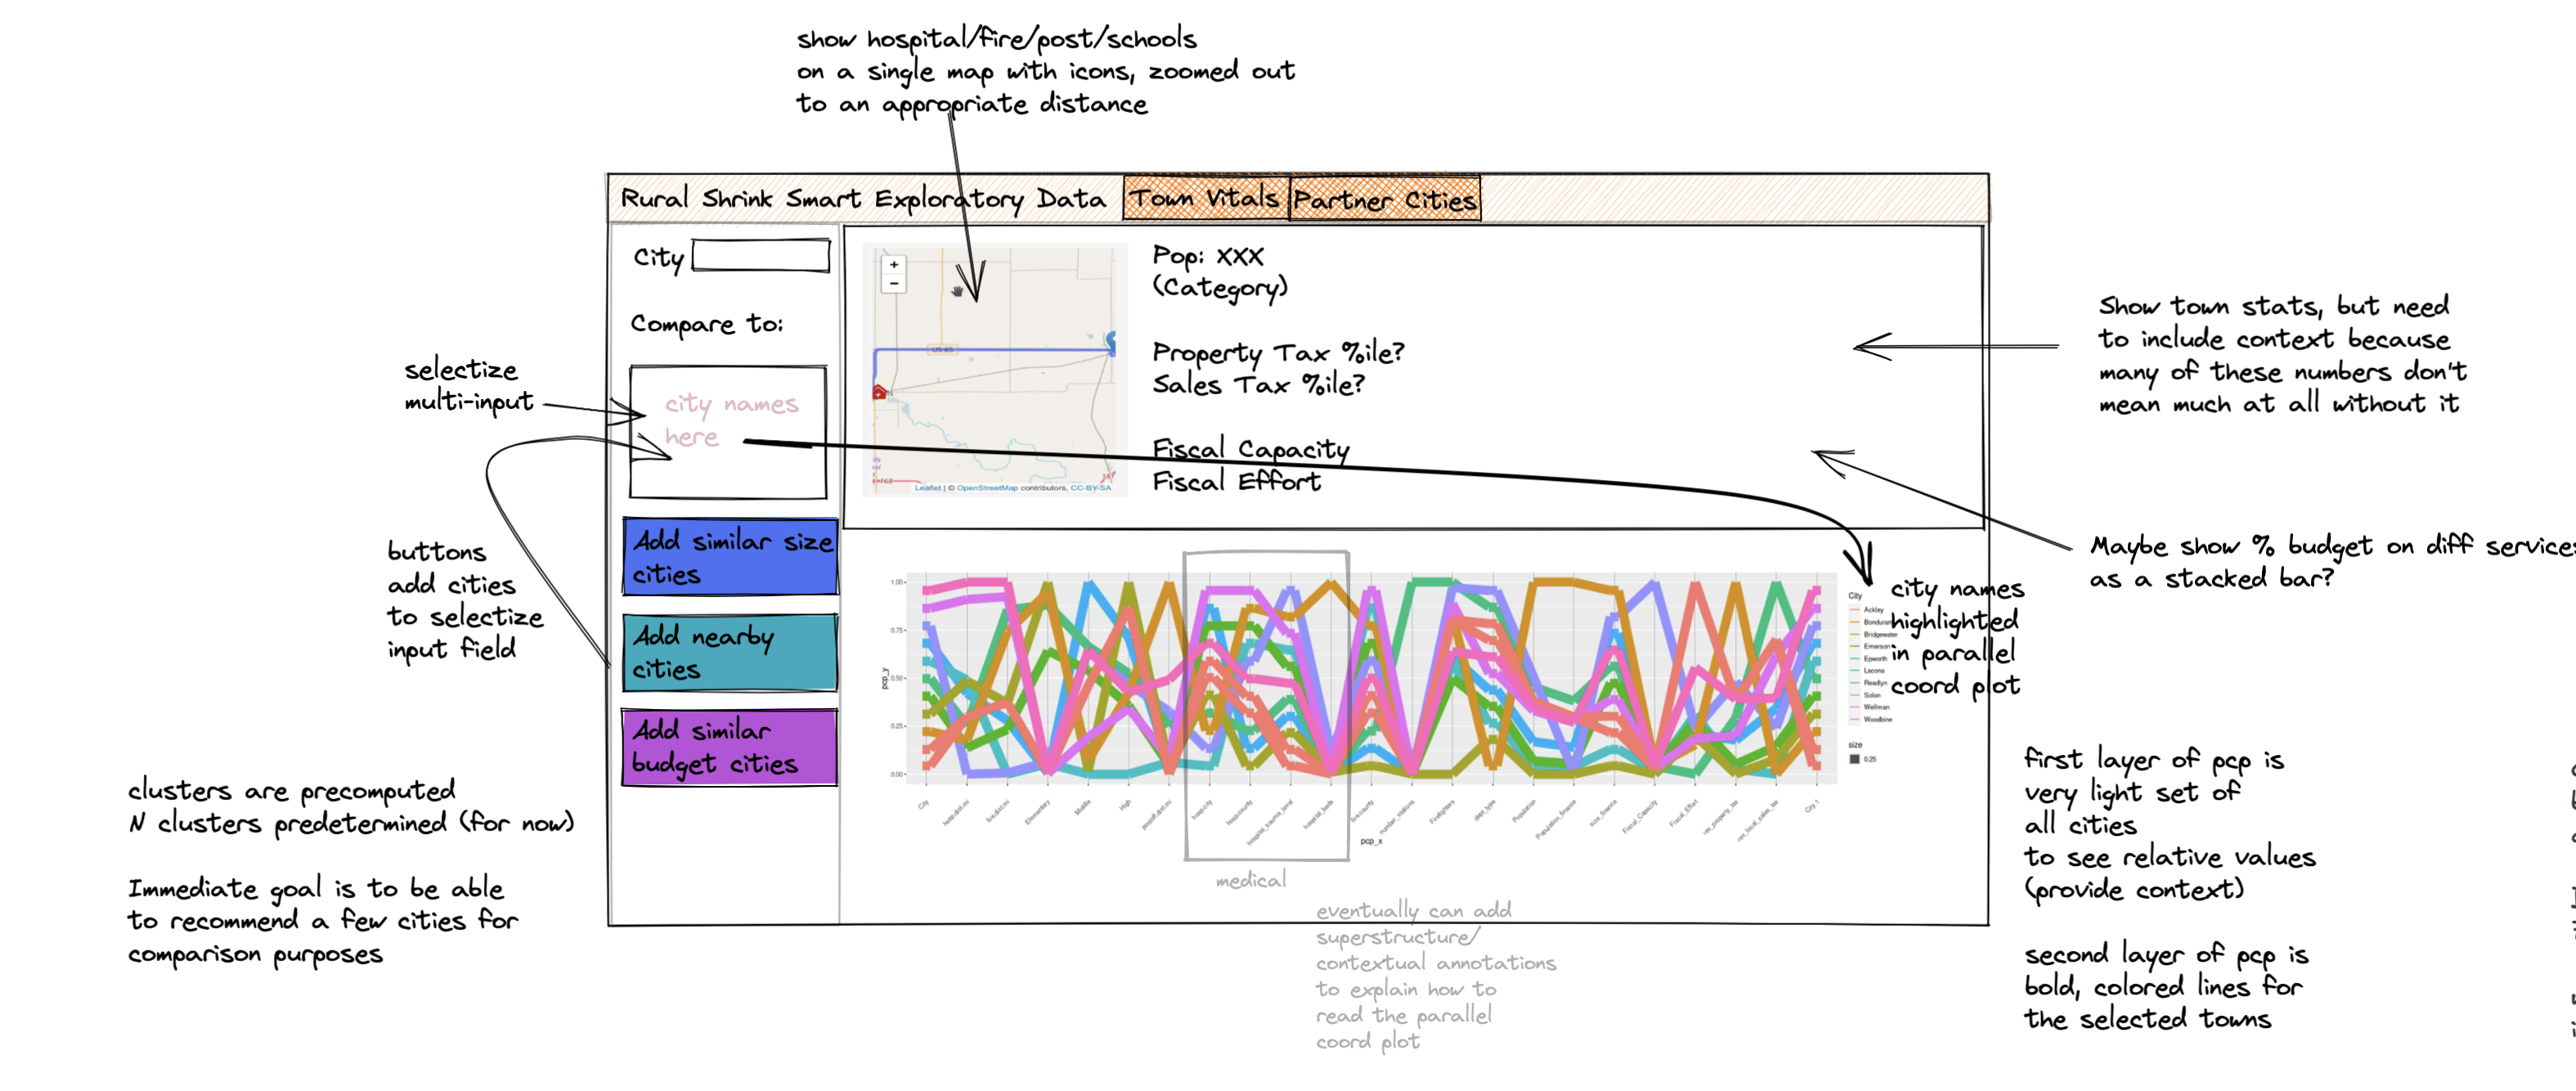
\includegraphics[width=\textwidth]{figure/Version1.png}

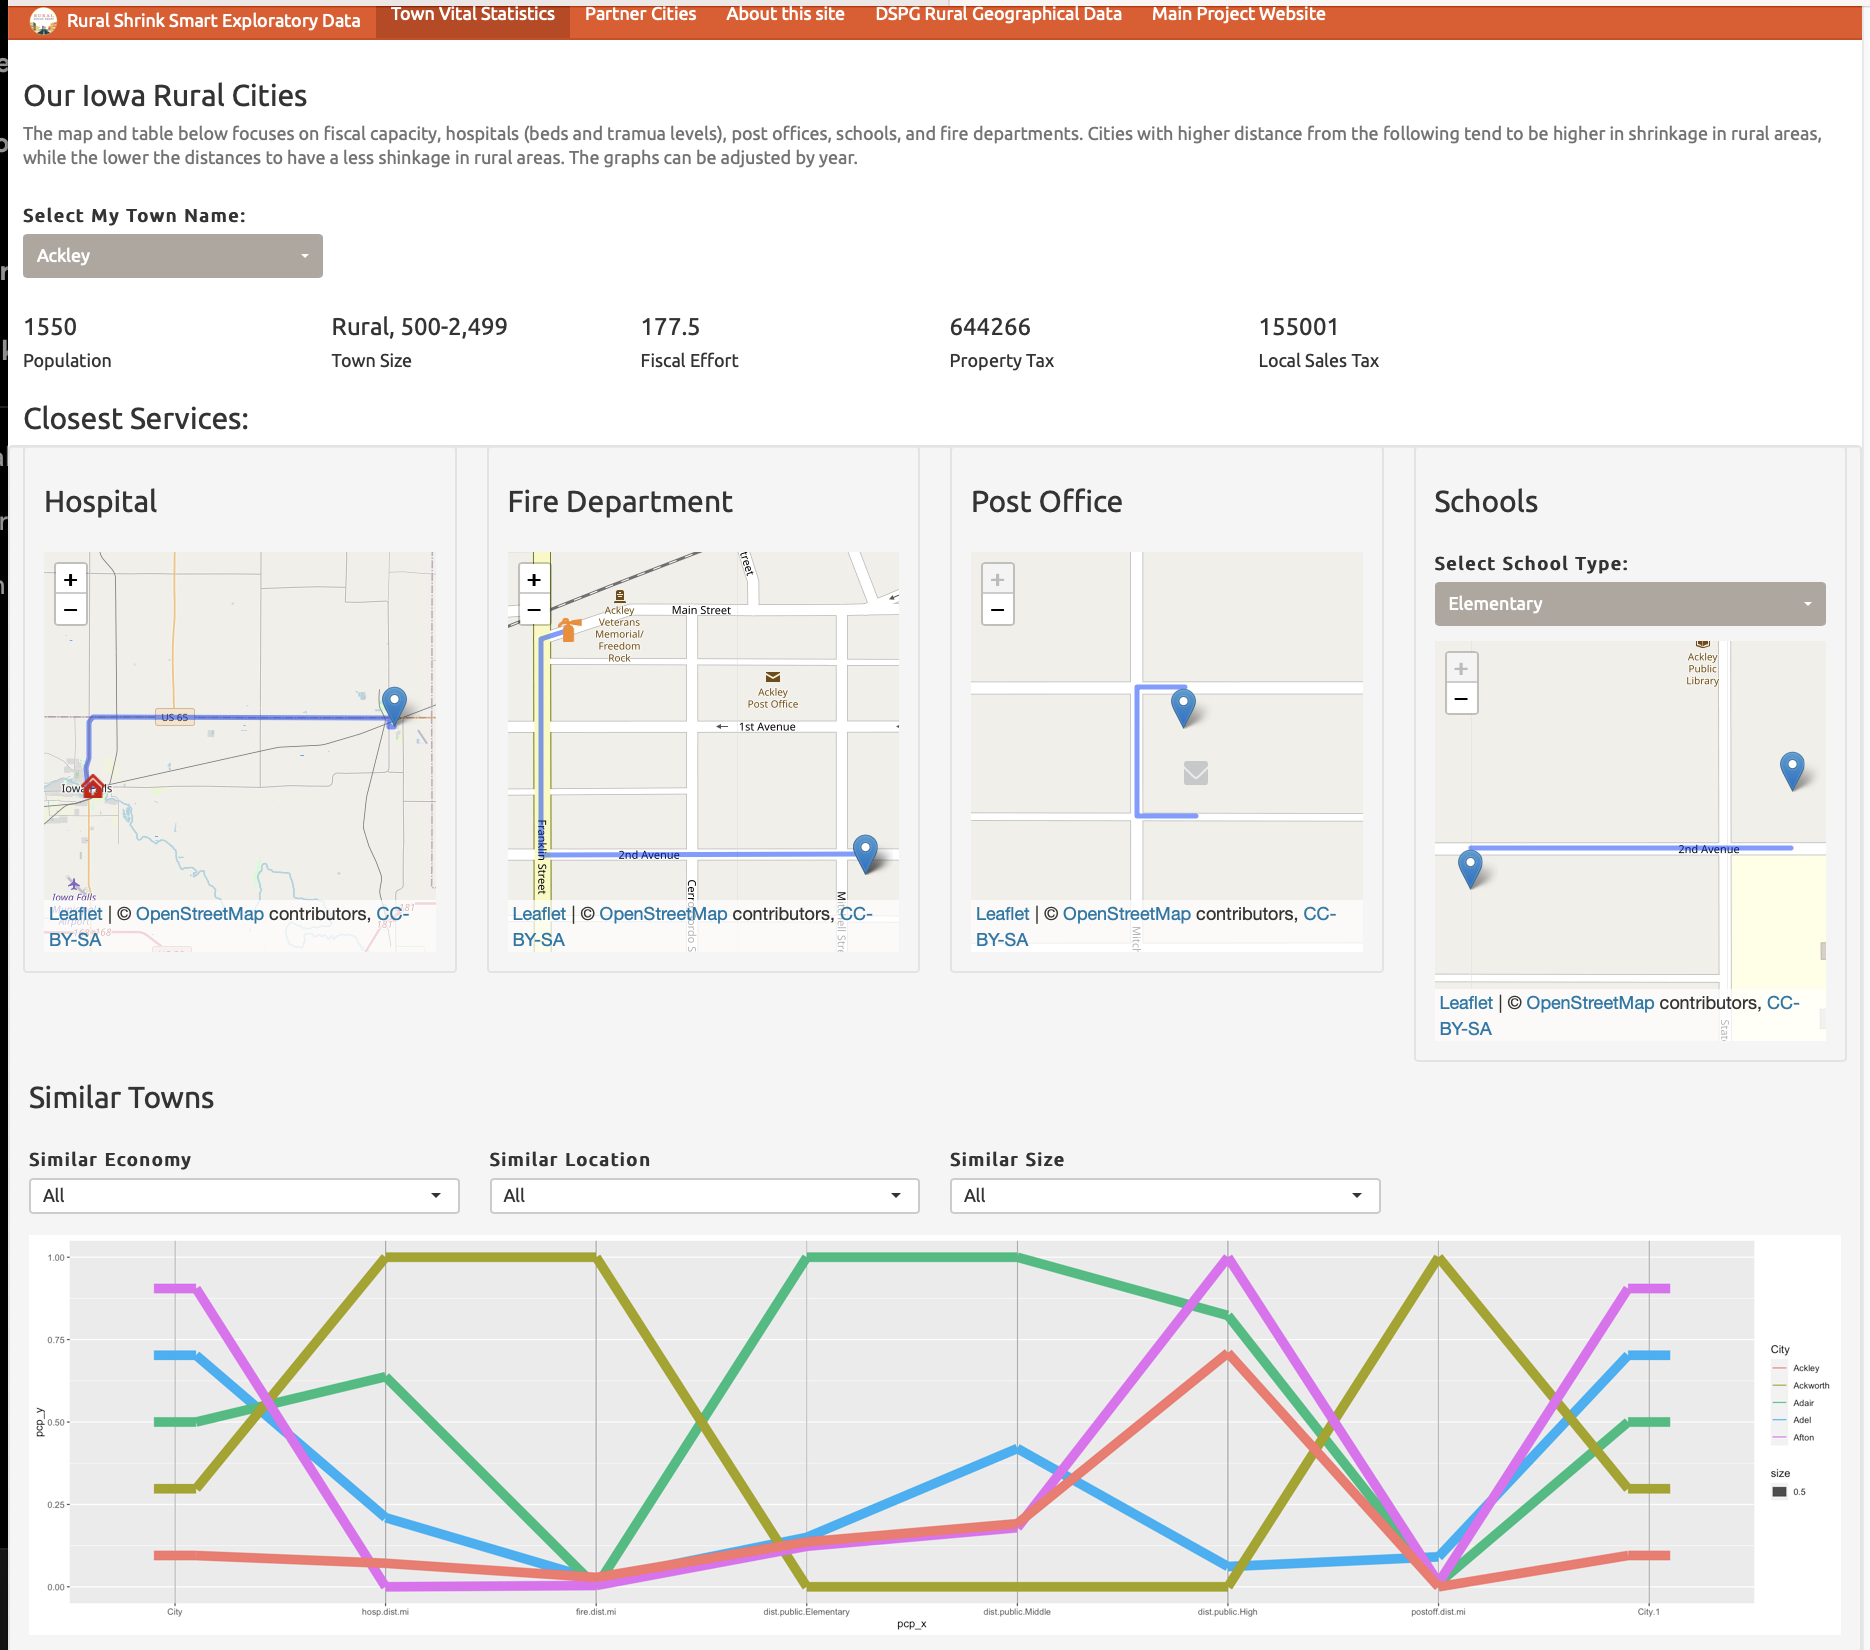
\includegraphics[width=.7\textwidth]{figure/Version2.png}
\caption{Initial dashboard design sketch (top) and implementation (bottom).}\label{fig:v1}
\end{figure}

We implemented some suggested town comparisons using unsupervised clustering methods to help our towns make decisions that are informed in comparison to similar towns, for budget size, population size and location. We initially focused on determining the next five to ten similar towns, based on distances to services. This feature became an important diagnostic for our data quality, as it became clear that towns which were grouped with big cities but which did not have a large population were so grouped because of missing data. Unfortunately, this clustering feature was not as useful to the application users, as they came to the dashboard with a pre-existing set of towns to compare to; our suggested comparisons were in the way.

The initial dashboard design featured several responsive maps showing the distance to the nearest hospital, fire department, post office, and school. These maps were ineffective for several reasons:

\begin{itemize}
\tightlist
\item
  Town residents already know this information (though it was useful for us as the dashboard designers, because we aren't nearly as familiar with the 900+ small towns in Iowa)
\item
  We computed distance from services relative to the center of town - coordinates provided in the data from \url{data.iowa.gov}. Generally speaking, the post office is at the center of town and the fire department is usually very close to the center of town; these two maps were useless. The school and hospital maps were less useless, but still did not provide particularly useful information to people already familiar with the town.
\item
  It became clear that it might be more useful to show the comparison towns on a map (relative to the town of interest) so that users could compare geographical ratings for unfamiliar data to familiar data.
\end{itemize}

In addition, we received feedback on the parallel coordinate plot at the bottom of the app which was surprising: the viewers (in this case, other researchers on the team) were not as intimidated by the parallel coordinate plot as we had expected. They did need some explanation of how to read the plot, and these hints need to be included in the dashboard, but they grasped the fundamental idea of the plot very quickly.

Our conclusion, based on this initial dashboard draft, was that we needed to restructure the application. Our attempt to show familiar information first to ``build up'' to the more unfamiliar structure of a parallel coordinate plot was not effective; there was too much clutter and not enough new information to draw users in.

\hypertarget{redesign}{%
\subsection{Redesign}\label{redesign}}

\begin{figure}
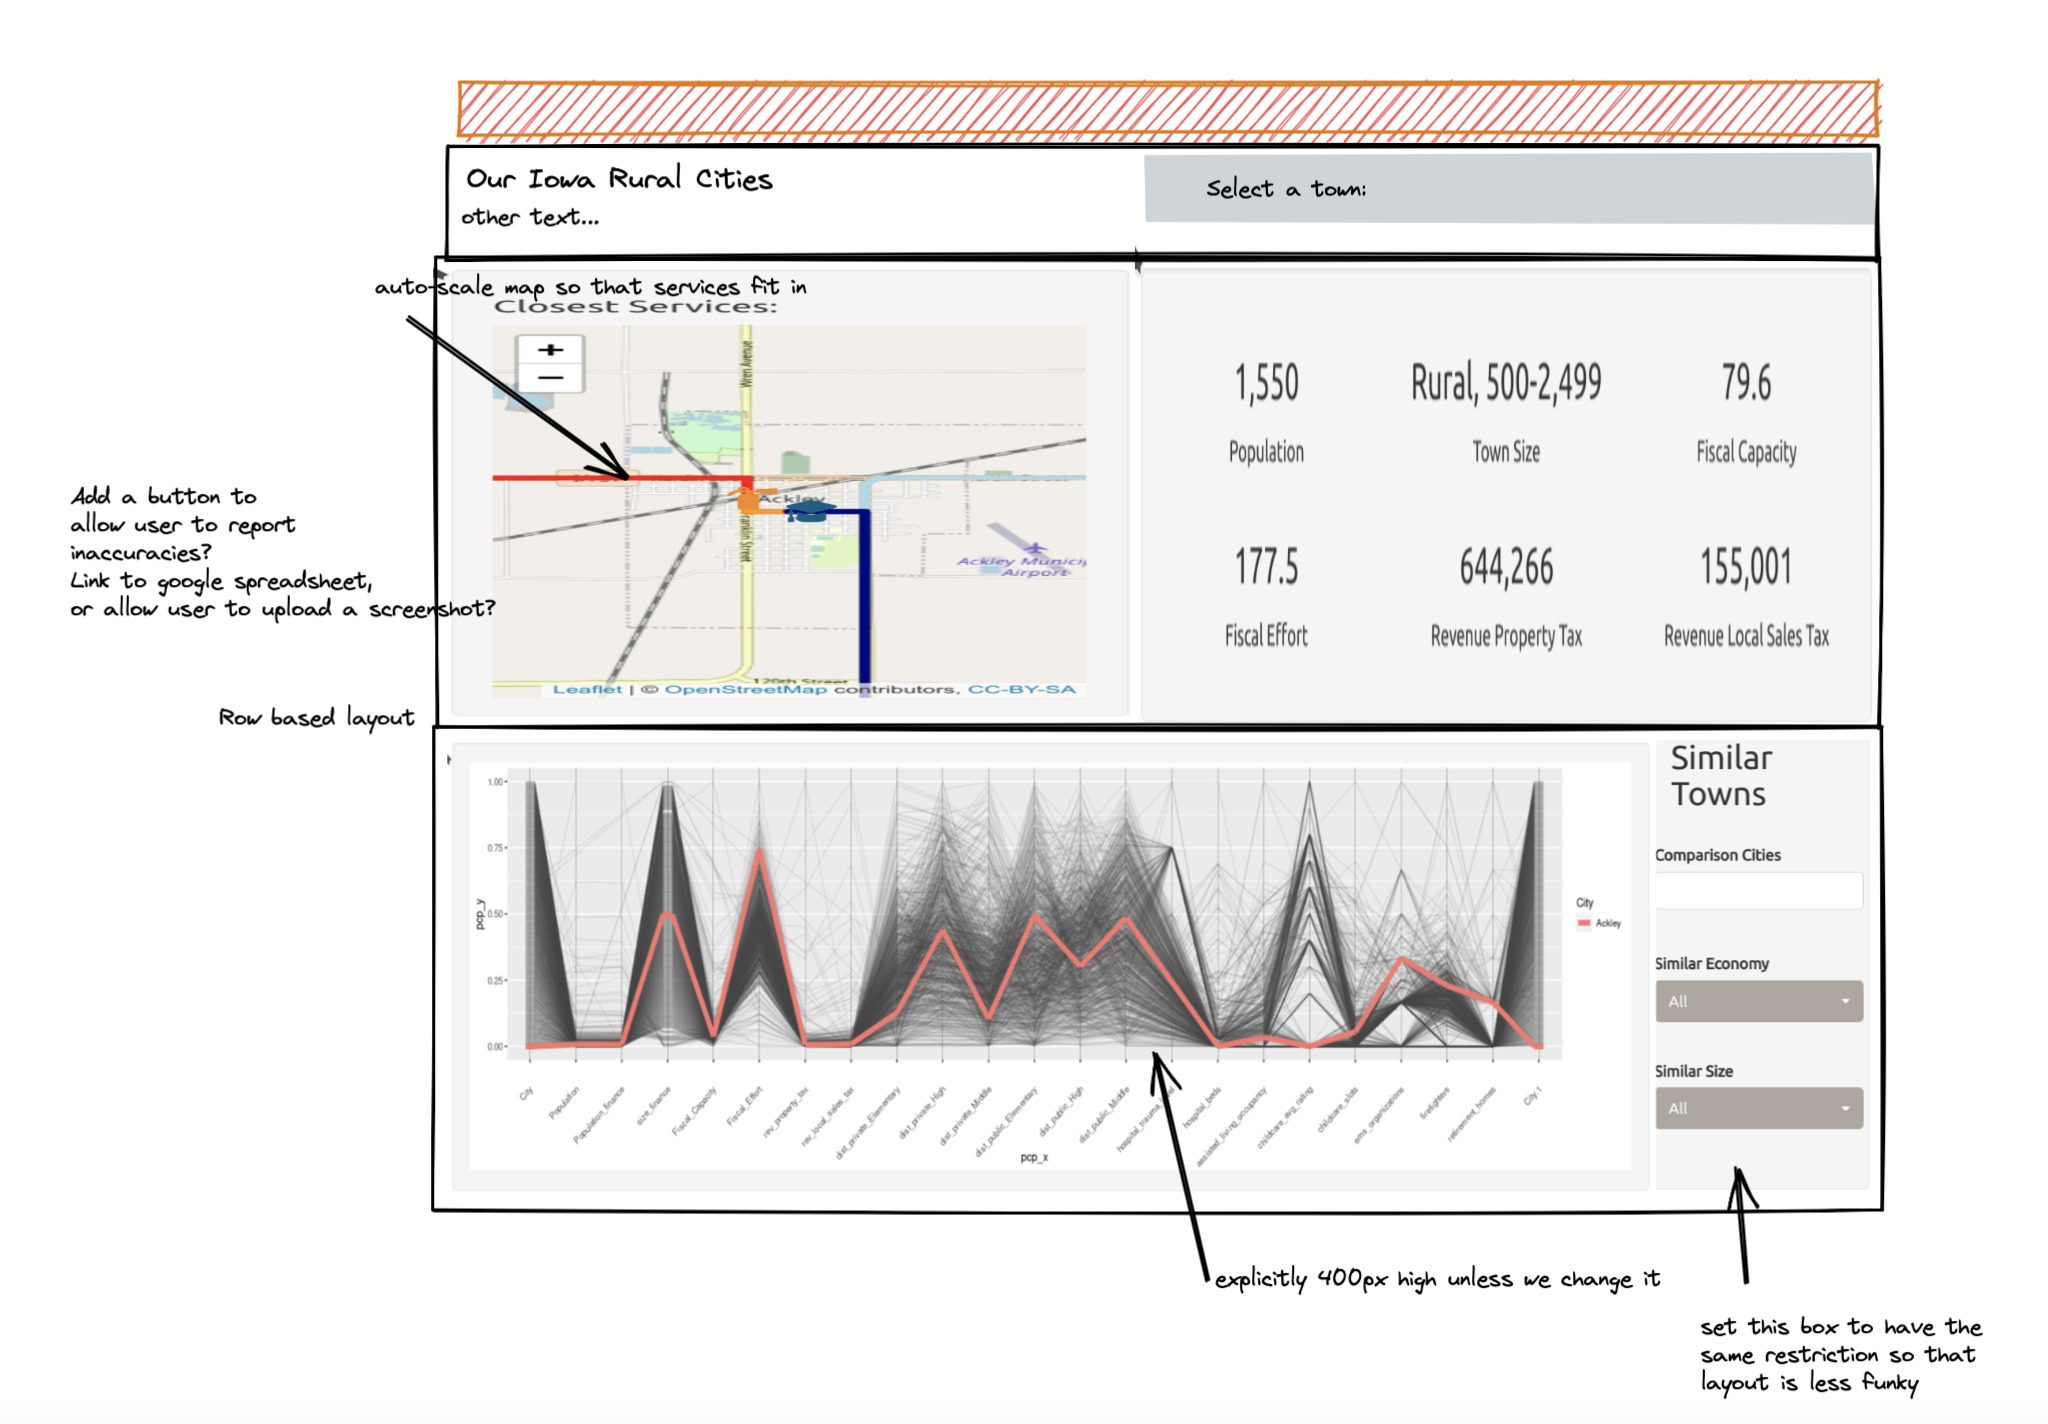
\includegraphics[width=.8\textwidth]{figure/Version3.png}

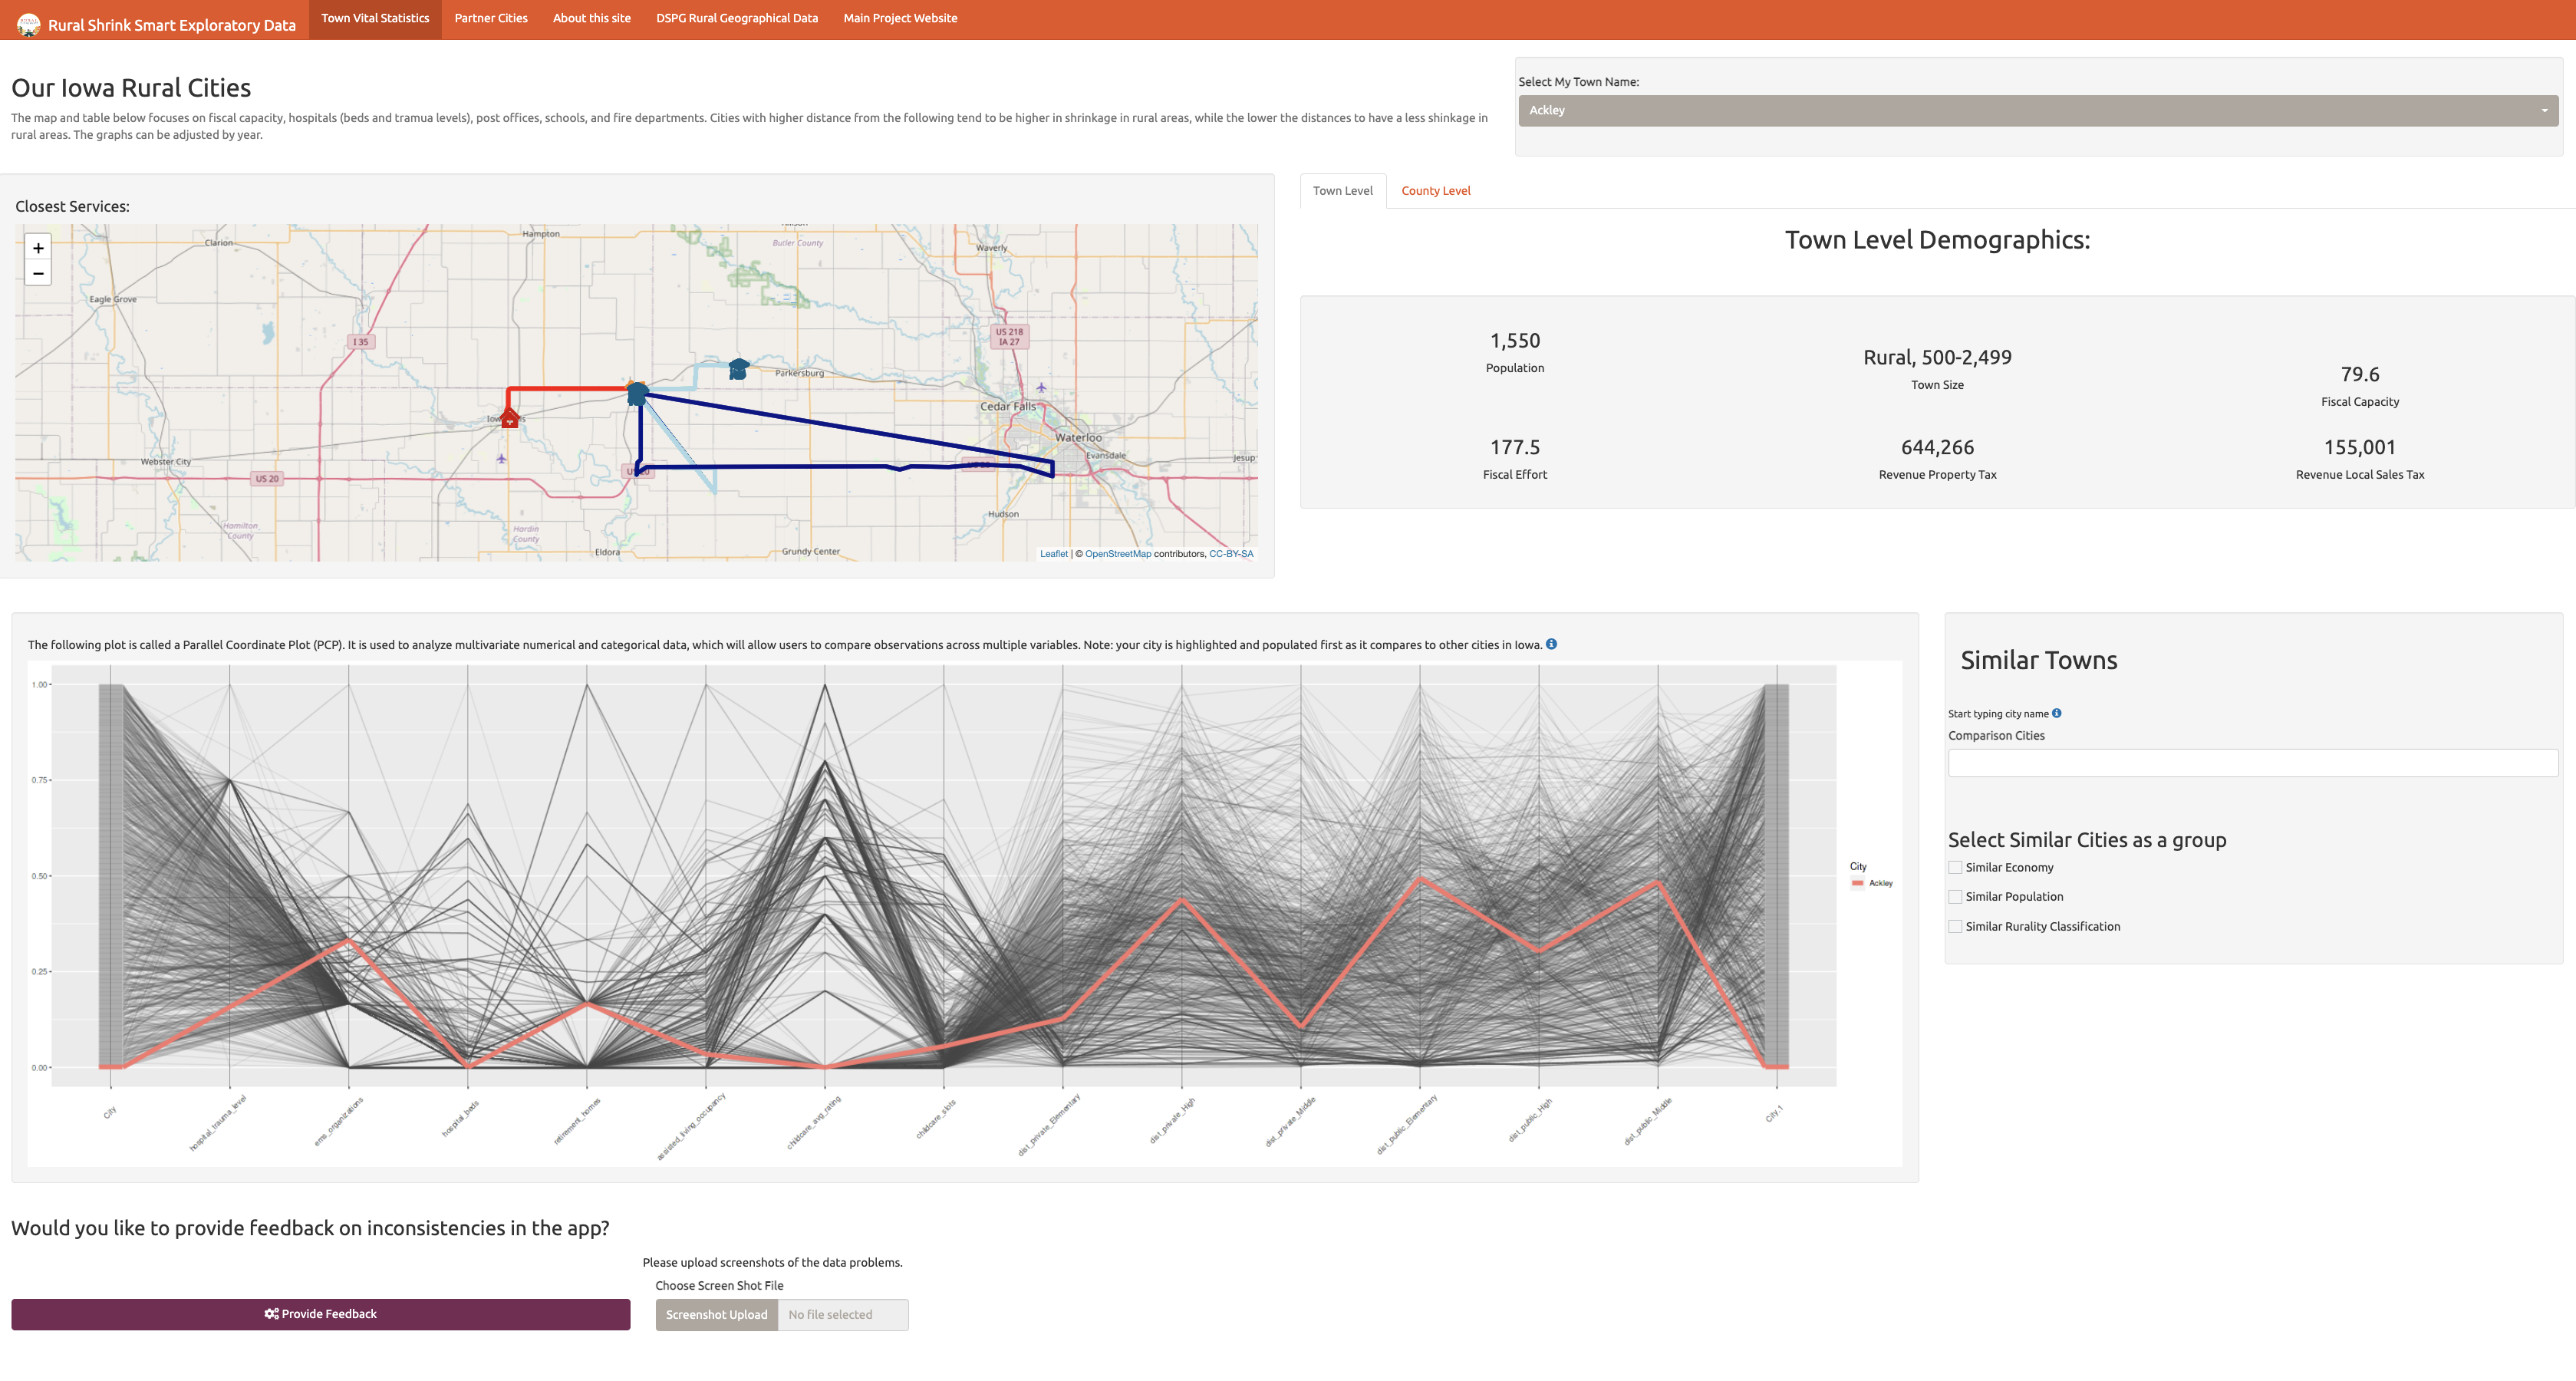
\includegraphics[width=\textwidth]{figure/Version4.png}
\caption{A second iteration of the sketched design (top) and the implementation (bottom).}\label{fig:v2}
\end{figure}

In the initial design, we included a map for each vital service, this initially created a lag for the users' experience. As a result, we cached map directions from OSRM for each service in our database, which drastically reduced the response time for the user. Our initial design did not naturally focus the user's eye on the most important parts of the dashboard; the redesign allowed for a cleaner flow from the top to the bottom.

In addition to the timing due to the map loading slowly, we added the vital statistics at the county level to allow for a more robust understanding of the town and it's surroundings. The rurality index provided a better classification and the USDA sources allowed for the town to understand the impact of the closest major city due to commuting for work and shopping at larger stores not available within the town.

We also modified the parallel coordinate plots in several ways:

\begin{itemize}
\tightlist
\item
  Our x-axis had a large number of variables that we as researchers believed to be the most strongly associated with quality of life. However, there were still too many variables for users to successfully parse. We reduced the number of variables, focusing on variables that had the highest data quality, and we grouped these variables by quality of life factor (Peters, 2019).
\item
  Originally, parallel coordinate bands were scaled based on the selected comparison towns. This had the effect of truncating the range of variables and over-emphasizing differences between selected towns relative to the overall range of each variable over all towns in our data set. We chose to show all towns in the data set in a very light \(\alpha\) grey color to provide some information about the overall range of each variable. Unfortunately, even with the low-\(\alpha\) value, this increased the visual complexity of the plot and confused users. Future iterations will likely make use of another aesthetic, such as boxplots or violin plots, to show the range of values for all towns, and then use lines only for towns that are selected by the user. This should strike a balance between visual complexity and representing the data accurately.
\item
  We noticed that users did not make use of our suggested comparison towns, and so we removed that option in favor of allowing users to enter their own comparison towns directly. Users already had pre-determined towns they wanted to compare to, and our suggestions were just in the way.
\end{itemize}

While not all of these modifications were well received in our second round of user testing, the changes did incrementally move the dashboard display towards our goal of allowing users to explore the data and engage with it. We continued to be surprised with how well users reacted to the parallel coordinate plots, which we initially thought might be too abstract for users unfamiliar with multivariate data displays, but the ability to compare towns across multiple dimensions and examine the similarities and differences between their approaches to different services seemed to be intuitive for users once they understood that each vertical axis was a different variable.

\hypertarget{discussion}{%
\section{Discussion}\label{discussion}}

Our dashboard design philosophy worked primarily to promote a town-centric approach application with comparisons to other similar towns being secondary. This approach created a way for the user to see their town information at the top of the page and to explore the PCP after reviewing their own town's essential statistics. The PCP in the lower part of the dashboard allowed for the user to see the plot and adjust to the fact that they could add more towns to the plot, providing an opportunity to explore the wider dataset from a base of familiar knowledge.

While we initially framed the design around guided discovery learning, the approach did not seem to suffice for our user base; instead, we found that users were more drawn to the unfamiliar from the start. We will likely leverage this in future iterations by using visual forms such as flower plots to draw the users in; even though these plots are not ideal for numerical display of data, the visual novelty and aesthetic appeal will provide some motivation to continue exploring and thinking about the data.

One factor that we have briefly considered and have seen hints of in our user feedback is that towns may not want to be compared negatively with other towns. While users have very definite ideas about which towns they would like to compare to, we can always mask the town names and move back to comparisons based on town size and other factors (for instance, whether or not a town is the county seat is a factor that is important outside of population). Using this approach, we would label each town as ``Town 1'', ``Town 2'', and so on, which would eliminate some of the fears about negative comparisons, but would also remove some of the novelty of the data dashboard for our users and would prevent users from drawing on their own outside knowledge about each of the comparison towns.

We also recognize that we need to leverage the expertise of others in our research team: we are working with artists, researchers in architecture, economists, and sociologists; these researchers provide outside knowledge that we do not have and may be able to help us create insightful use-cases to showcase the app and teach towns how to use it. We can also leverage the app to connect users with our research team, providing additional value to those who use the applet and facilitating development of strategies for maintaining quality of life amid shrinking populations.

\hypertarget{future-work}{%
\section{Future Work}\label{future-work}}

One avenue we will explore in future iterations of the dashboard is to incorporate other dashboards generated by different groups within this project. This will create a wider field of information to explore: for instance, some of the additional work will focus on the 99 towns featured in the Iowa Small Town Poll; this will allow us to showcase survey-based measures of quality of life alongside the more objective measurements assembled in the dataset discussed in this paper. While at least one tab of this omni-dashboard will still focus on wider EDA and discovery, we hope to incorporate other information as well to provide a more well-rounded data display encompassing most of the facets of this complex project.

We are also mindful of a distinction between ``eye candy'' and purpose-driven data visualization. While we have typically focused on the latter, there is certainly a place in our dashboard for the former as well. ``Eye candy'' visualization is intended to draw the viewer in and motivate them to explore; while these visualizations may not be particularly effective at communicating quantitative information, if they motivate the user to engage with the rest of the dashboard, they still serve a purpose. It is with this mindset that we intend to explore the use of flower plots - the artistic opportunities combined with the display of quantitative information (even in a form that isn't optimal for quantitative comparisons) may be useful to engage viewers before transitioning to more useful data visualizations intended to provide accurate quantitative comparisons.

EDA can be a difficult for a variety of groups of people, novice users and experienced researchers. One of the more difficult components of this project has been clearly articulating the purposes of EDA to a diverse group of researchers unfamiliar with the concept. One of the most useful parts of this dashboard iteration process has been as an aid to data discovery: that is, the dashboard motivated us to find additional data sources and incorporate them into the project. Having conversations with other researchers about the EDA process helped to facilitate these conversations, as each discussion seemed to uncover additional data sources that someone remembered after looking at the dashboard. While this facet of the dashboard process may be difficult to study formally, it would be an interesting avenue for investigation.

\hypertarget{conclusions}{%
\section{Conclusions}\label{conclusions}}

In this paper, we have documented the process of designing a dashboard for exploration and visualization of a large and complex data set assembled from many different sources. Our primary audience was leaders of small towns in Iowa, with a secondary audience of researchers in fields other than statistics collaborating on this project with us. Through the process of revising our dashboard, we found that the idea of guided discovery learning as implemented in our first version did not work as well as we had anticipated. It was more important to focus on allowing users to explore their questions about the dataset by facilitating user-driven comparisons and exploration, rather than attempting to anticipate user desires by providing comparison towns. In addition, we found that it would be more effective to draw users in with novel visual displays, as these seemed to attract more interest than providing known facts and an opportunity to explore outwards from an initial area of familiarity.

While it is hard to apply the findings from one fairly specific visualization project more widely, there is a lack of resources in this area that provide both design philosophies and actual analysis of user feedback in a qualitative sense. We have attempted to address this dearth of information by providing the design strategies, user feedback, and our planned and executed modifications, in the hopes that others facing the daunting challenge of designing a dashboard for EDA may learn something from our experiences.

\hypertarget{math-sci}{%
\chapter{Dashboard Poetry}\label{math-sci}}

\hypertarget{introduction-2}{%
\section{Introduction}\label{introduction-2}}

Statisticians use graphs in almost every stage of their work.
They create charts to summarize and explore new data and identify potential problems and opportunities (Tukey \& Wilk, 1966).
Models are fit based on relationships between variables which are often identified visually (Hullman \& Gelman, 2021).
We identify problems with those models based on residual plots and other visual diagnostics.
When our modeling work has been completed, we present our results to interested parties using visual displays, because non-statisticians often find it easier to understand data and models through an intuitive visual medium rather than through the mathematical formulae which underlie the statistical work.

When we create visualizations for public consumption, we have to consider both perceptual factors and the target audience's domain knowledge.
In addition, not all visual displays have equal perceptual value Aspillaga (1996).
The best graphics are designed to account for both the dataset and the intended audience's features.
Some design constraints stem from limitations of the human perceptual system and are common to most potential consumers of the visualization.
For example, the sine illusion affects anyone with binocular depth perception, and color recommendations are built around the specific characteristics of the human retina (VanderPlas \& Hofmann, 2015b).
Other design constraints are due to the audience's experience level and if they are used to working with data and understand specialized techniques (e.g., enough familiarity with principal component analysis such that a plot of factor loadings might be useful).
Given the wide range of uses for graphs and visual data displays in statistical modeling, it is unsurprising that some graphs are more useful for specific applications, such as exploratory analysis, and are unsuitable for other applications, such as presenting to an outside group.

Most research in statistical graphics has been done on static graphics; usually, research also strips away all but the most essential contextual information, sacrificing external validity for statistical control.
As a result, it can be hard to generalize this research to practical applications, where the contextual information surrounding the data is critical and the chart does not just exist in a vacuum.

In the real world, however, conventions and familiarity often win out over best practice validated by perceptual experiments.
In ``The Commercial and Political Atlas,'' Playfair used various types of graphical representations to illustrate economic and political data.
He included a chart that he called a ``circle chart'' or ``pie chart'' to display the distribution of imports and exports of England in 1781 (Playfair, 2005).
Scholars frequently choose to utilize pie charts as a means of presenting data, acknowledging the widespread familiarity of this particular chart format among readers (Edward R. Tufte, 2001).
Discrete categories can be effectively highlighted by their utilization.
Moreover, researchers have the ability to enhance the accessibility of their study findings to a broader range of individuals.
However, there are certain limitations that should be acknowledged.
Pie charts may not be appropriate for visualizing datasets that have a large number of categories or require precise comparisons.
This is because it can be difficult to precisely perceive slight differences in the sizes of the pie chart's wedges.
In addition, the presence of inaccurate labeling and scaling has the potential to result in misinterpretation.
Hence, it is imperative for researchers to exercise prudence while utilizing pie charts as a visualization tool for categorical data, in order to guarantee precise and significant portrayal.

Dashboards have seen a significant increase in day-to-day usage as a potent data visualization and decision-making tool.
The John Hopkins COVID-19 Dashboard is a reputable online platform that offers current and comprehensive data and statistics pertaining to the worldwide COVID-19 epidemic.
The tool mentioned earlier functions as a highly helpful instrument in monitoring the dissemination of the virus, providing up-to-date information on the prevalence of cases, fatalities, and immunization rates within various nations and geographical areas.
This dashboard is widely utilized by researchers, politicians, and the general public as a reliable and authoritative resource for continuously monitoring the ongoing effects of the epidemic ({``John hopkins university covid-19 dashboard,''} n.d.).
The proliferation of dashboards can be attributed to several factors, including the growing availability of data from various sources and the increasing need for organizations to extract actionable insights.
Steven Few found that the widespread use of dashboards is attributable to their capacity to present key performance indicators and relevant metrics in a visually appealing and easily digestible format, (Few, 2006b).
Moreover, technological advancements and the development of user-friendly dashboard platforms have facilitated the creation and effective utilization of dashboards by individuals from diverse fields.
Dashboards have revolutionized data analysis and presentation, allowing users to gain valuable insights and make data-driven decisions more effectively.

Each chart on the dashboard contributes to the overall comprehension of the situation, similar to how each sentence in a paragraph contributes to the larger concept.
A chart is similar to a sentence in that it presents a straightforward piece of information and visually represents data to facilitate comprehension.
For example, a chart could be a bar graph depicting sales over a year, a pie chart illustrating the percentage distribution of a budget, or a scatter plot illustrating the correlation between two variables.
A dashboard may combine multiple graphs, tables, and metrics to provide an all-encompassing view of a company's performance, a project's development, or market trends.

However, a counterexample to this analogy could be a poorly designed dashboard presenting overwhelming information without clear organization or hierarchy.
In such a case, the charts may compete for attention and confuse the reader, similar to how a paragraph with too many disjointed sentences can lead to confusion and a lack of coherence.
This counterexample highlights the importance of thoughtful design and effective communication in creating an informative and comprehensible dashboard.
The research objective of this study is to investigate how changes in real-time data displayed on a dashboard affect ensemble perception and the user's ability to make accurate and rapid decisions based on summary statistics in a dynamic environment.

John Tukey was the first to organize the collection and methods associated with philosophy into exploratory data analysis (EDA).
Tukey used graphics as a tool for exploratory analysis.
In ``Exploratory Data Analysis,'' Tukey wrote that graphics and charts often display data with more enhanced understanding than a table (Tukey \& Wilk, 1966).
Tukey outlines in detail the types of different graphics and in which situations to utilize them.
He was a strong advocate for the importance of EDA as a crucial first step in the data analysis process and emphasized the need for visualization and interactive techniques to understand patterns and relationships in data.

John Tukey's exploratory data analysis (EDA) principles revolutionized the way we approach data exploration and visualization, emphasizing the importance of understanding data's underlying structure and patterns before diving into formal statistical analysis.
Tukey's Principles in EDA:

\begin{enumerate}
\def\labelenumi{\arabic{enumi}.}
\item
  Through graphic exploration (looking for patterns or displaying fit), the method demonstrates things about data that a single numeric metric does not understand.
  This has been useful in graphing the data before you develop summary statistics.
\item
  Describing the general patterns of the data This step should be insensitive to outliers.
  In general, think about the types of resistant measures (i.e., median or mean).
  This step makes sure to determine data patterns.
\item
  The natural scale or state in which the data are at their best.
  This will be the step at which the scale of the data can be helpful for analysis.
\item
  The most known part of EDA is done by assessing the fit of the data.
  This is taught in every statistics 101 class.
  With the growth of machine learning and prediction methods, residuals are now more widely used in the toolbox for assessing the best prediction models.
\end{enumerate}

Tukey's Principles of EDA have become a cornerstone in the field of statistics and have been adopted by data professionals in various industries.
Tukey's principles have enabled data professionals to understand complex data sets better and make more informed decisions by emphasizing the importance of visual exploration, data characterization, and model critique.
In this way, Tukey's Principles have revolutionized our data analysis approach and become the foundational framework for EDA.

\begin{center}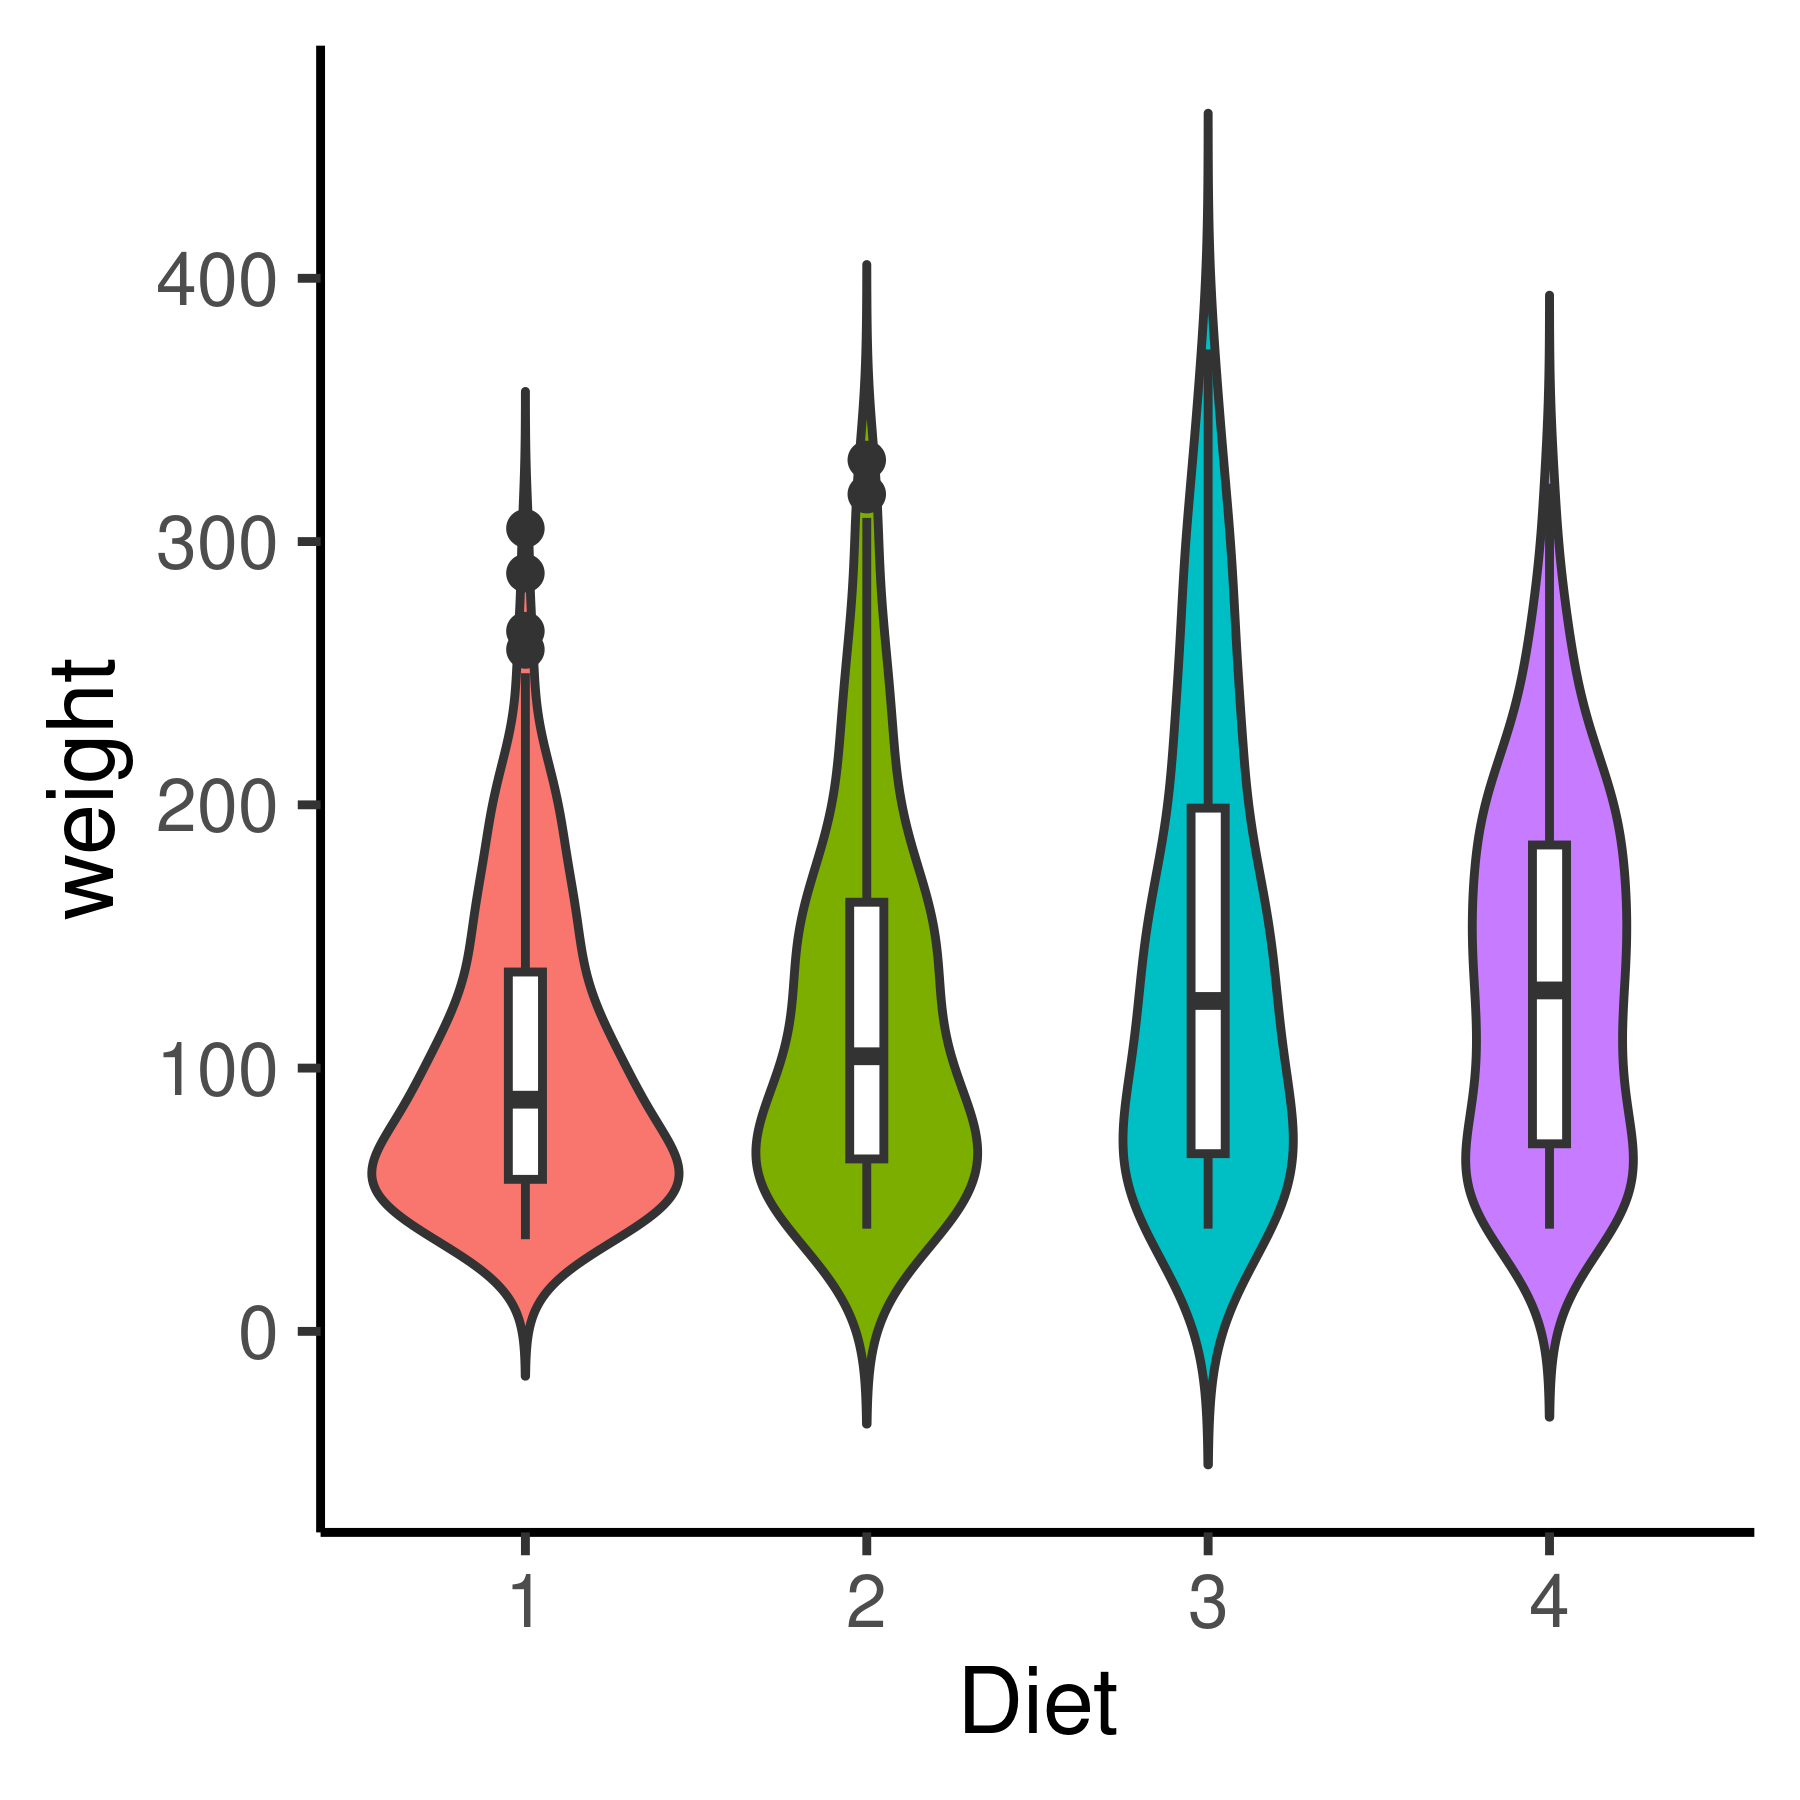
\includegraphics[width=.49\linewidth]{thesis_files/figure-latex/unnamed-chunk-1-1} \end{center}

\begin{center}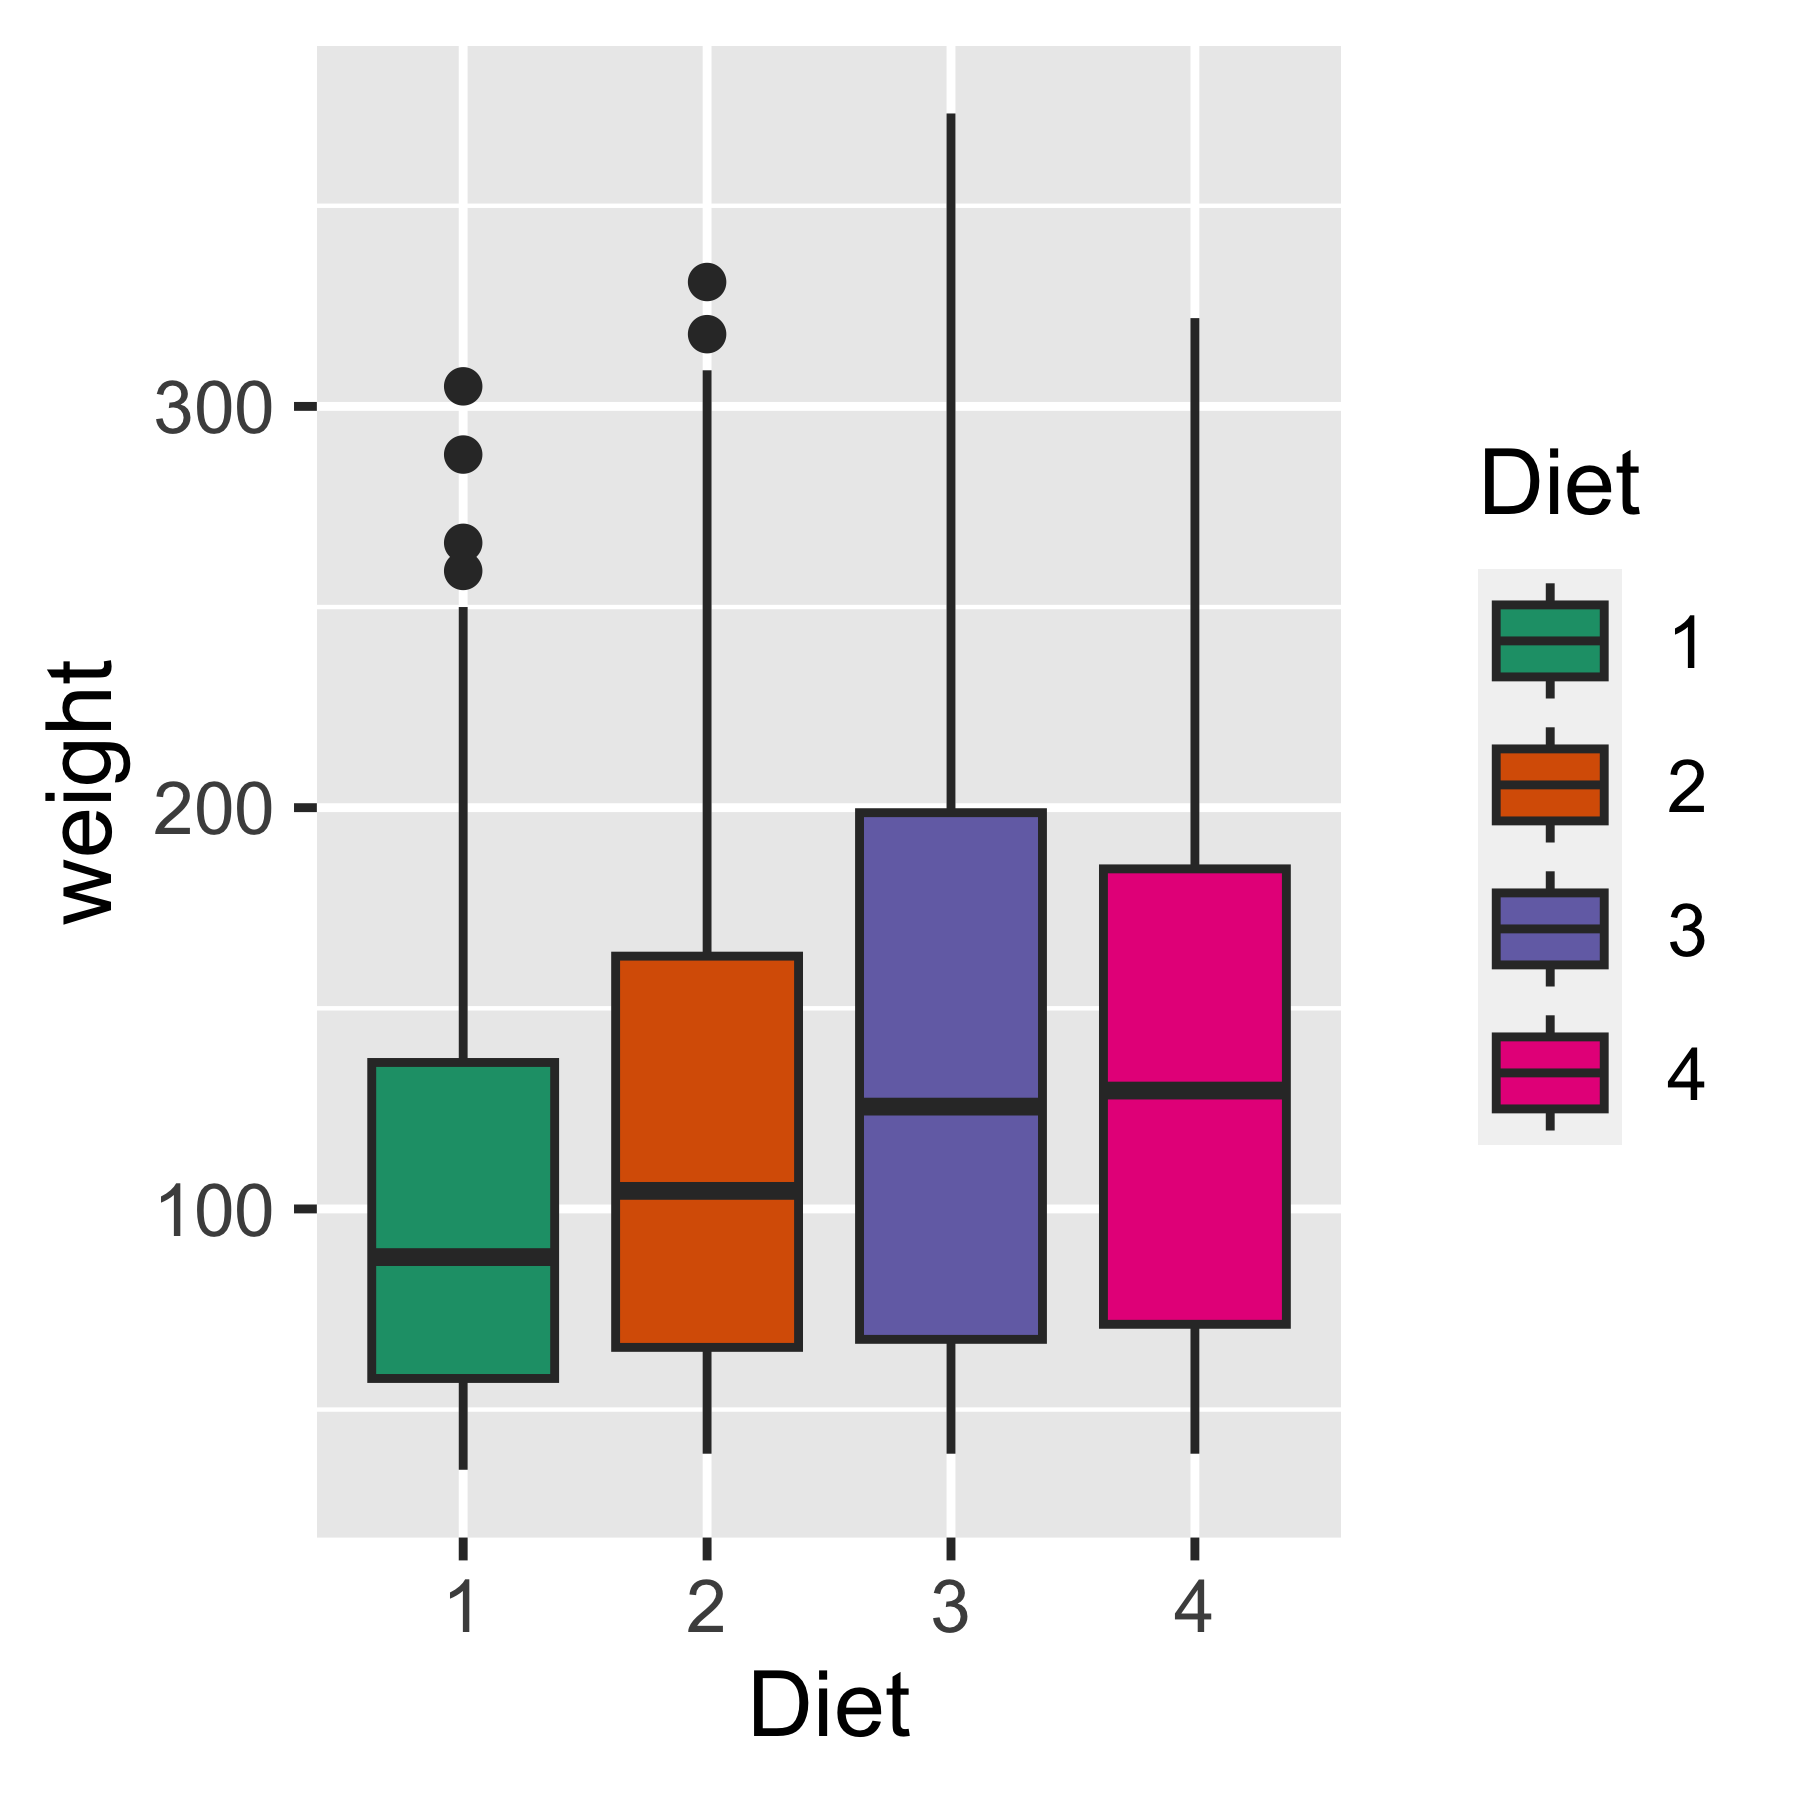
\includegraphics[width=.49\linewidth]{thesis_files/figure-latex/unnamed-chunk-1-2} \end{center}

Data visualizations are an integral part of the EDA process, enabling analysts to discern patterns and relationships in the data that would otherwise be difficult to discern from tabular data alone.
Through data visualization, analysts can quickly identify trends, outliers, and other patterns that may be missed through numerical analysis alone.
Visualizations facilitate the communication of findings to non-technical stakeholders, allowing them to comprehend complex data sets more efficiently.
Also, analysts can use visualizations to identify potential issues or biases in the data, resulting in better decisions and models.

Using color to represent data on maps is an example of successful graphical communication utilizing semiology.
By using different colors to represent different data points, viewers can comprehend patterns and relationships in the data quickly and easily.
Jacques Bertin writes in ``Semiology of Graphics'' that color can be used to ``emphasize a point, distinguish one category from another, or establish a relationship between two points'', (Monmonier, 1985).
In addition, Bertin explains that the use of color can help overcome language barriers, making it easier for the audience to comprehend the presented information.

By utilizing visual elements such as bars and lines to represent data, graphs can make complex information more understandable to viewers.
For instance, a line graph can be used to illustrate the change in the value of a stock over time, making it easier for investors to identify trends and patterns.
Leland Wilkinson writes in his book ``The Grammar of Graphics'' that ``graphical methods are not only superior to other forms of communication but also superior to numerical or verbal methods for certain types of data and reasoning'' (Wilkinson, 2012).

It proposes that any statistical graphic can be broken down into a set of essential components, or ``grammar,'' that can be combined in different ways to create a wide range of visualizations, following a layered approach to describe and construct visualizations or graphics in a structured manner.

The components of the grammar of graphics include:

\begin{itemize}
\item
  Data: The raw data being visualized represents a set of observations or values.
\item
  Aesthetic Mappings: The mapping of data variables to visual properties such as position, color, shape, and size.
\item
  Scales: The mapping of data values to visual values, such as mapping a numerical value to a bar height.
\item
  Geometries: The basic shapes representing the data, such as points, lines, bars, and histograms.
\item
  Facets: The plot division into multiple subplots, each representing a different subset of the data.
\end{itemize}

For example, a bar chart can be created by mapping a categorical variable to the x-axis, mapping a numerical variable to bar heights, and using rectangular bars as the geometry.
Moreover, mapping two numerical variables can create a scatter plot to the x and y positions and use points as the geometry.
Finally, the ``Grammar of Graphics'' provides a systematic way of thinking about visualizations, making it easier to choose the appropriate visual representation for a given dataset.

\begin{figure}

{\centering 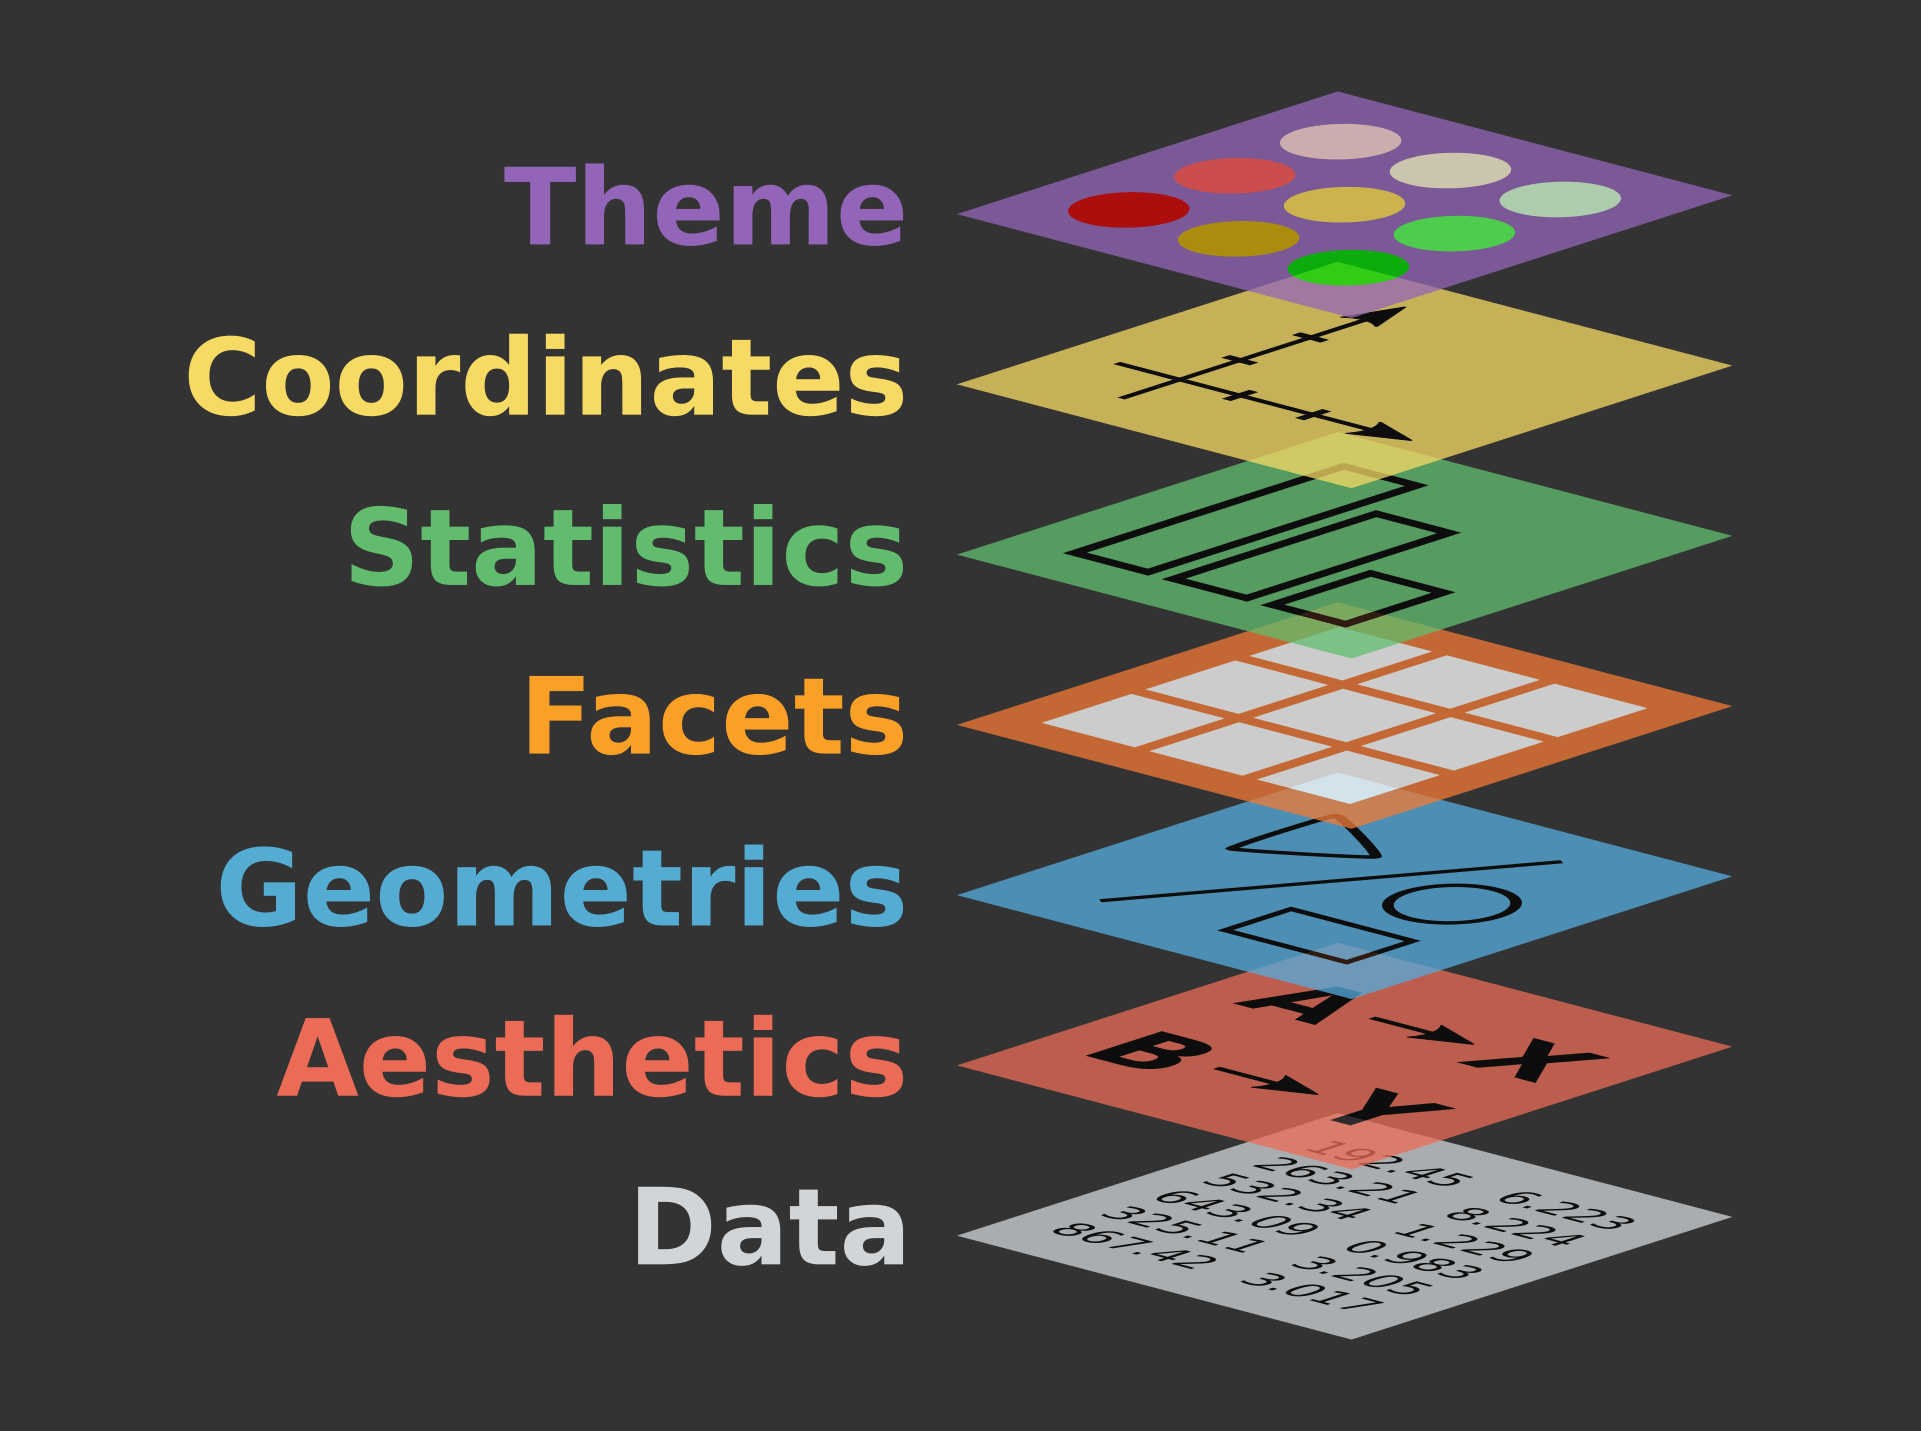
\includegraphics[width=0.45\linewidth]{figure/gglayers} 

}

\caption{Grammar of Graphics Diagram of Wickham and Wilkinson's work}\label{fig:unnamed-chunk-2-1}
\end{figure}
\begin{figure}

{\centering 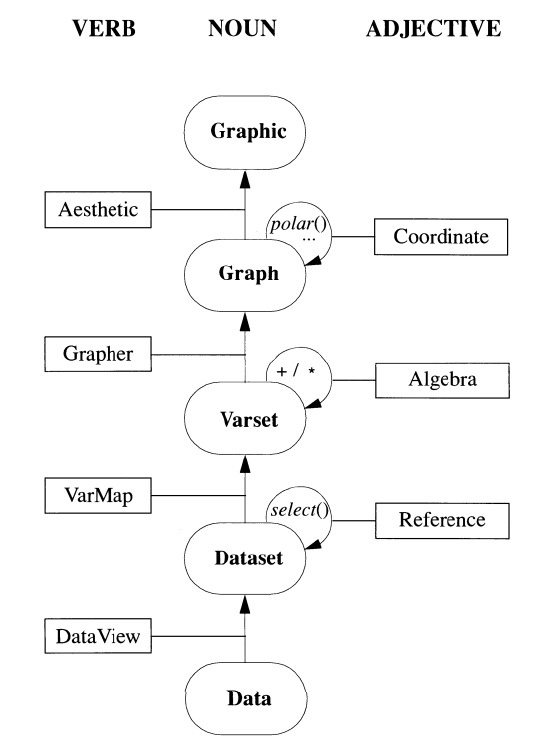
\includegraphics[width=0.45\linewidth]{figure/graphic-flowchart} 

}

\caption{Grammar of Graphics Diagram of Wickham and Wilkinson's work}\label{fig:unnamed-chunk-2-2}
\end{figure}

A dashboard is a visual display of the essential information needed to achieve one or more objectives, consolidated and arranged on a single screen so the data can be monitored at a glance (Few, 2006b).
Dashboard design creates visually informative and interactive interfaces that present data and key performance indicators (KPIs) in a consolidated and simple-to-understand format.
The objective of KPIs are to provide users with insights and enable them to make intelligent decisions based on the presented data.\\
As organizations increasingly rely on data-driven decision-making, well-designed dashboards become pivotal.\\
The literature on dashboard design provides a comprehensive roadmap for understanding and implementing effective dashboards, focusing on critical applications such as evaluation criteria in healthcare, learning dashboards in educational settings, design patterns and trade-offs, academic literature reviews, and practical tips for implementation.
Each of these applications offers unique perspectives and actionable insights.
If the data used in the design and implementation of dashboards is flawed or incomplete, it can lead to misleading insights and ineffective decision-making.
Additionally, different user groups' specific needs and preferences may not always align with the applications provided.

A systematic literature review by (Schwendimann et al., 2016) discusses the state-of-the-art in learning dashboards.
The paper identifies critical design features, dividing them into functional and visual features.\\
This study is particularly useful for educational institutions implementing learning analytics dashboards.
Conducted as a systematic literature review, the study categorizes critical design features into functional and visual aspects, providing a comprehensive understanding of what makes a learning dashboard effective.
By identifying key design elements and their impact on student performance, the paper is a foundational resource for educators and administrators looking to leverage dashboards to enhance educational outcomes.

\hypertarget{dashbaord-construction}{%
\section{Dashbaord Construction}\label{dashbaord-construction}}

Given that the intended audience has limitations, there are design constraints around the data, and the audience has the ability to successfully use the graphical displays of the data, what can we take from this body of research that applies to more complicated sets of graphics?
How do we maintain user attention, create a desire to explore, and accurately communicate the data through the medium of an interactive data dashboard?
Solutions to these questions can start with a dashboard.

A dashboard is a visual display of the essential information needed to achieve one or more objectives, consolidated and arranged on a single screen so the data can be monitored at a glance (Few, 2006b).

Dashboards can present various statistical data, such as financial performance, website traffic, or customer engagement metrics.
They allow users to quickly and easily understand complex data sets by using visual elements such as charts, graphs, and tables to display the information.
Additionally, statistics can be used to analyze data presented on a dashboard, providing insights into trends and patterns that can inform decision-making.

While a dashboard can be handy, it may be worth mentioning that a poorly designed dashboard will not be used.
A dashboard should be concise, clear, and intuitive when displaying components in combination with a customized list of user requirements.

Much of the work done in statistical research and dashboard design involves collaboration with other researchers and users.
While this may be the best for the growth of the discipline, one will find that working with collaborators with non-STEM backgrounds Dashboards can help understand and support many data types for essential business objectives.
There are many different ways to label and utilize dashboards of different kinds.

Combining two compelling graphics does not necessarily result in a successful visualization.
In certain instances, suboptimal combinations can result in confusion, misinterpretation, and the failure to convey the intended message. Combining two charts with distinct scales or units is an example of suboptimal graphic design, which can result in misinterpretation and flawed comparisons.\\
For example, if a bar chart displaying the number of sales is combined with a line chart showing revenue, meaningful comparisons between the two metrics can be challenging.
According to a study conducted by Cleveland and McGill, people frequently make inaccurate judgments when comparing graphs with different scales (Cleveland \& McGill, 1984).

In addition, combining two difficult-to-compare graphics with redundant visual cues or unnecessary embellishments such as colors, 3D effects, or patterns can increase cognitive load and reduce the dashboard's effectiveness.
Although adding extra elements to a chart or graph may be tempting, doing so can detract from the primary message and make it more difficult for the audience to focus on the essential information.
Tufte discovered that adding unnecessary visual cues to a graph decreases its effectiveness because viewers are more likely to focus on the embellishments rather than the data (Edward R. Tufte, 1985).
Most importantly, dashboards should leverage people's visual and cognitive capabilities.

Static Visualization is commonly used in the communication phase of data science workflows, and data scientists sometimes use them as part of the analysis.
John Tukey's EDA methods are currently known and well-vetted in the field.
However, Satyanarayan et al.~addressed this by introducing a high-level grammar of graphics called ``Vega-Lite,'' which presents a set of standardized linguistic rules for producing interactive information visualizations using a concise JSON format for data to be represented by the grammar (Satyanarayan, Moritz, Wongsuphasawat, \& Heer, 2016).
Vega-Lite has been directly implemented in R via the \texttt{ggvis} package using the same - albeit slightly lower-level.

Understanding cognitive load is crucial for designing compelling data visualizations, as it influences how users perceive, process, and remember the data presented in the visualization.
When designing visuals, it is essential to consider the cognitive load they may place on the viewer.
Cognitive load is the amount of mental effort required to process information, and minimizing it can enhance a graphic's effectiveness.
In addition, displaying as much raw data as possible while minimizing cognitive load can improve the graphic's clarity and precision.
Here are some general guidelines for making better graphics with works from Few (\textbf{few2012?}), Tufte (\textbf{tufte1983?}), and Cairo (Cairo, 2016):

\begin{enumerate}
\def\labelenumi{\arabic{enumi}.}
\item
  Keep it simple - Avoid overwhelming the viewer with too much information at once by employing a clear and concise design with minimal distractions.
\item
  Use visual hierarchy - Utilize size, color, contrast, and placement to highlight important information and direct the viewer's focus.
\item
  Choose appropriate charts - Choose the chart type that best illustrates the data and facilitates comprehension.
\item
  Label clearly - Use labels that are clear and concise for axes, legends, and other essential information to avoid confusion.
\item
  Use data-to-ink ratio - Focus on the data by minimizing the amount of non-data ink, such as decorative elements or excessive grid lines.
\item
  Avoid distortion - Use appropriate scaling and avoid distortions to ensure that the graphics accurately represent the data.
\item
  Provide context - Add context to assist the viewer in comprehending the significance of the data and its relevance to the topic.
\end{enumerate}

These principles are based on cognitive psychology and understanding how the human brain processes visual information.
Cowan suggested that the average person can only hold two to six pieces of information at a time (Cowan, 2001).
By applying these principles to dashboard design, designers can create visual arrangements that make it easier for viewers to understand the relationships between data elements.
For example, proximity can be used to group related elements together, while symmetry can be used to create balance and harmony in the overall layout of the dashboard.
At its most basic, the entire form is perceived (or emerges from our visual pathways) as opposed to its component parts.
For instance, if a scatter plot and a bar chart are combined, the resulting visualization may be difficult to interpret due to the two graphics types' incompatibility.
Hullman et al. (Hullman, Adar, \& Shah, 2011) discovered that viewers had trouble understanding a visualization that included a scatter plot and a line chart, which brought attention to this issue.
Moving forward, designers must navigate the delicate balance of complexity and comprehension to ensure that dashboards serve as a potent tool for conveying information succinctly and effectively, enhancing the viewer's ability to grasp and analyze the presented data seamlessly.

\hypertarget{cognitive-principles}{%
\section{Cognitive Principles}\label{cognitive-principles}}

Perception is a biological process involving sensory systems and neural mechanisms.
The retina, a multi-layered tissue, lines the back of the eye and converts photons into electrical impulses that travel along the optic nerve to the brain.
This process is crucial for understanding perception.
Sensory modality, such as sight, hearing, and touch, has specialized receptors that convert physical stimuli into electrical signals that the brain can interpret.
For instance, light enters the eye and activates photoreceptor cells in the retina, (Hubel \& Wiesel, 2004).

\begin{figure}

{\centering 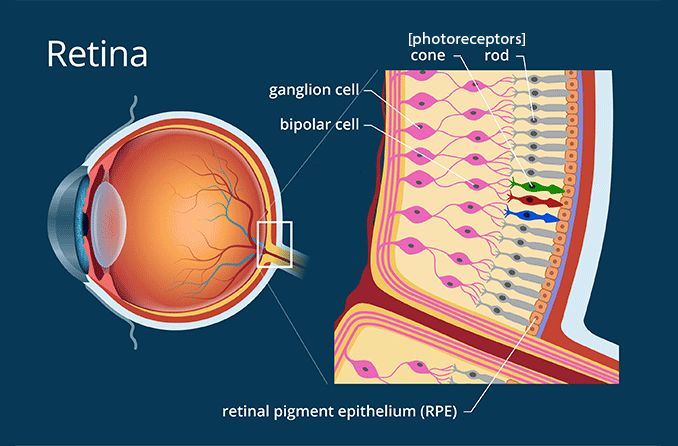
\includegraphics[width=0.55\linewidth]{figure/photoreceptors_image} 

}

\caption{An example of how the retina signals the visual cortex}\label{fig:unnamed-chunk-3}
\end{figure}

Human perception is an essential component of data visualization that can significantly enhance both the content and quantity of displayed information (Ware, 2012).
Perception refers to the organization, interpretation, and conscious experience of sensory data.
Perception is also defined as ``the process of recognizing (being aware of), organizing (gathering and storing), and interpreting (binding to knowledge) sensory information'' (Ward, Grinstein, \& Keim, 2010).
Ward et al.~explain the notion of perception as follows: ``The brain makes assumptions about the world to overcome the inherent ambiguity in all sensory data and in response to the task at hand.''

The principles of eye-tracking involve the investigation of eye movements and fixations during visual perception.
Eye-tracking technology permits researchers to monitor and record where individuals look and how their gaze traverses a visual scene.
This data can be utilized to analyze patterns of attention, gaze behavior, and the sequence of fixations.
The principles of eye-tracking provide valuable information regarding how individuals allocate their attention, which elements attract their gaze, and how they visually explore and process information.

Gestalt principles, on the other hand, examine how humans perceive and organize visual elements into meaningful patterns and wholes.
These principles originated in the field of Gestalt psychology, which emphasized that perception is influenced by the arrangement and grouping of its constituent parts.
The Gestalt principles of proximity, similarity, closure, and continuity describe how our brains organize visual stimuli to form coherent and meaningful perceptions.

Perceptual grouping is a fundamental process in visual perception that involves organizing individual graphical elements into coherent perceptual units based on their inherent properties and spatial relationships.
It helps us make sense of the complex visual world by grouping elements that belong to the same object or structure and separating elements that belong to different entities. Gestalt psychologists have extensively studied the concept of perceptual grouping, proposing principles such as proximity, similarity, closure, and continuity as grouping's underlying mechanisms.~
These principles govern our perception of objects, edges, contours, and patterns, enabling us to perceive organized and meaningful visual information (Wertheimer, 1938), (Wagemans et al., 2012) and (Palmer, 2002).

The Gestalt principles play a crucial role in directing eye movements and cognitive processes involved in scanning scenes.
The integration of scene scanning with Gestalt grouping concepts synergistically contributes to the facilitation of visual scene perception and comprehension.
In the course of scene scanning, individuals frequently employ Gestalt grouping principles, such as proximity and similarity, in an unconscious manner to arrange diverse visual elements into cohesive groups.
This process facilitates the rapid and efficient interpretation of intricate scenes (WERTHEIMER, 1923) and (Wertheimer, 1938).
They facilitate the efficient assimilation and processing of visual information by emphasizing specific clusters or patterns in the visual field.

Scene scanning is the cognitive process of visually examining a given scene in order to acquire relevant information pertaining to the surrounding environment.
The aforementioned procedure encompasses the utilization of both ocular motions and cognitive mechanisms to comprehend and analyze the visual data inherent in a given scenario.
The subject matter is frequently examined within the framework of disciplines such as psychology, neuroscience, and computer vision.

The process of exploring visual scenes involves an intricate interaction of cognitive processes that influence an individual's perception and interaction with their surroundings.
The saliency-driven focus is a key mechanism that guides scene scanning.
This process involves both overt and covert shifts of visual attention, which are directed towards specific characteristics in the environment.
Itti and Koch have extensively studied and explained this phenomena.
Furthermore, the cognitive processes involved in perceiving scenes frequently involve a higher-level comprehension that entails a synergistic equilibrium between bottom-up processes driven by stimuli and top-down strategies driven by information (Itti \& Koch, 2000).
This theoretical perspective is supported by the work of Henderson and Hollingworth (Henderson \& Hollingworth, 1999).
The aforementioned phenomena are applicable to various cognitive processes such as reading, visual searches, and scene perception, as demonstrated by (Rayner, 2009).
In this study, it was found that eye movements during these activities are notably impacted by individual cognitive processes, including linguistic comprehension and visual interpretation.
Moreover, the interpretation and allocation of attention during scene scanning are influenced by the context in which visual items are encountered, as emphasized by (Bar, 2004).
The significance of global features in the search for objects in real-world settings is crucial for guiding eye movements and attention within a contextual framework, (\textbf{torrablba2006?}).

By examining the complexities of scene scanning, it becomes evident that attention plays a crucial role in directing the eyes systematically as they analyze and comprehend the visual narratives present in each gaze.
This process contributes to a complex cognitive framework that integrates perception and interpretation through an interactive and dynamic relationship.

Starting with Wertheimer's experiments on the perception of motion, he examined the phenomenon of apparent motion, which refers to the perception of motion when successive stationary stimuli are presented.~
Wertheimer investigated the principles underlying the perception of motion and provided insights into the Gestalt principles of visual perception by conducting a series of perceptual experiments.

(Wertheimer, 1912) investigated the phi motion, a type of motion in which the rapid presentation of two stationary stimuli creates the perception of movement.
By manipulating the temporal and spatial arrangement of stimuli systematically, Wertheimer was able to identify critical factors that influenced the perception of motion.
His experiments revealed that motion perception results from the interaction between sensory input and perceptual organization processes.

The work of Wertheimer emphasized the significance of perceptual grouping principles, such as proximity and similarity, in the perception of motion.
He hypothesized that the visual system tends to group stimuli that are close in space or have similar properties, resulting in the perception of a continuous and smooth motion between them.
The results of Wertheimer's experiments on the perception of motion were instrumental in developing Gestalt psychology, which emphasized the significance of holistic and organized perceptual experiences.
Wertheimer's work influenced our understanding of how the brain processes visual information to create motion perception by laying the groundwork for subsequent studies on motion perception.

According to (Goldstein \& Cacciamani, 2021), preattentive processing automatically extracts and analyzes basic features such as color, shape, orientation, and motion.
These features are processed in parallel across the visual field, allowing for the rapid detection and identification of salient environmental stimuli.
Preattentive processing occurs effortlessly and outside conscious awareness, laying the foundation for subsequent attentional selection and more elaborate perceptual processing.

The theories of Goldstein emphasize the significance of preattentive processes in various perceptual domains.
For instance, he discusses the preattentive analysis of visual features such as color and orientation, which contribute to the visual perception of objects, scenes, and graphic patterns.
In the auditory domain, preattentive processes automatically extract basic acoustic features like pitch and loudness.
This makes it easier to find the source of sounds and tell them apart.

By examining preattentive processing, Goldstein's theories provide a framework for comprehending the initial stages of sensory processing and the automatic extraction of fundamental perceptual features.
These theories have significant implications for understanding how automatic and controlled processes shape perception.~

Perception and attention are crucial cognitive processes that allow users to interpret and make sense of data visualizations.
Perception refers to the manner in which we interpret and organize sensory information from our environment, whereas attention refers to the capacity to selectively focus on particular aspects of this information (McCallum, n.d.).
Expectations of perception and attention are important in data visualization interactions, however expertise is the in-depth knowledge and skills that come from having a lot of experience and learning over a long period of time.

In addition to perception and focus, domain-specific knowledge is essential for understanding and interacting with data visualizations.
Expertise in a particular field can enable individuals to better interpret and comprehend the significance of the presented data, as well as identify potential biases or errors in the visualization.
Thus, the ability to perceive and interact with data visualizations requires a combination of perceptual and attentional processes, as well as domain-specific knowledge, to interpret and comprehend the presented information.
This suggests that data visualization involves the misuse of human visual perception in the visual presentation of data.
Assigning meaning to visualization is not a statistical or computational step but a cognitive one.
Each step in the data analysis process is part of a more extensive mental process of constructing meaning with important cognitive-based concepts.

Short-term memory (STM), which is often referred to as working memory, represents a cognitive stage characterized by the brief storage and processing of information, requiring significant cognitive resources for memory preservation.
In the publication titled ``Working memory: Theories, models, and controversies'' authored by Alan Baddeley, it is asserted that short-term memory (STM) is a system with restricted capacity that is susceptible to both interference and decay (A. Baddeley, 2012).
Selective attention plays a crucial role in the preservation of short-term memory (STM) since it enables individuals to effectively filter out extraneous information and focus on pertinent stimuli (Cowan, 2001).
According to (Alvarez \& Cavanagh, 2004), the utilization of visual aids, such as charts and diagrams, has the potential to enhance short-term memory by facilitating more efficient encoding and retention of information.
The utilization of visual aids, such as charts, has the potential to increase our short-term memory.
Moreover, annotations can also serve to facilitate short-term memory.
According to (Alvarez \& Cavanagh, 2004), the act of incorporating annotations, such as notes or highlights, to the information we aim to retain can enhance our ability to recall the information at a later time.

According to the Feature Integration Theory (FIT), STM is composed of two stages: pre-attentive processing and focused attention (A. Treisman, 1998).
Parallel and independently, the brain processes the physical characteristics of an object, such as its color, shape, and orientation, during pre-attentive processing.
However, focused attention is required to bind these features into a coherent object representation in STM.
STM can be improved through various strategies, such as rehearsal, chunking, and elaboration (Oberauer, 2009).
For example, by repeating a phone number several times or breaking it down into chunks of two or three digits, we can increase the likelihood of it being stored in STM.
Similarly, by elaborating on the information we want to remember, such as creating mental associations or visual images, we can enhance its retention in STM (Bui \& Myerson, 2014).

STM is a dynamic and malleable cognitive system that is crucial to our daily lives.
Understanding the mechanisms underlying STM and how to improve it can have significant implications for learning, memory, and the treatment of memory disorders.
By analyzing the relationship between attention and working memory, we can gain insight into how we construct meaning from the information in our environment.

Gestalt psychology indicates that humans actively construct meaning by organizing information into patterns and wholes (Wertheimer, 1938).
Both top-down and bottom-up processing are involved in the process of meaning construction.
Bottom-up processing entails analyzing sensory data from the environment and constructing perceptions based on this data.
Top-down processing reflects the influence of prior knowledge, expectations, and context on the perception and interpretation of incoming sensory data.

Together, top-down and bottom-up processing facilitate the encoding and retrieval of information from STM.
Selective attention, which is the ability to focus on relevant information while ignoring irrelevant information, is an example of top-down processing that aids in the encoding and retrieval of information in STM (Cowan, 2010).\\
According to FIT, perceiving objects involves both the bottom-up analysis of individual features and the top-down processing of higher-level features in order to form a complete perception (A. M. Treisman \& Gelade, 1980).

The Gestalt principles of perception address how humans construct meaning from sensory data through both bottom-up and top-down processing.
Both types of processing are involved in encoding and retrieving information, which has significant implications for understanding the mechanisms of STM.

Baddeley expanded our understanding of working memory by emphasizing its active processing nature, expanding upon the model of Atkinson and Shiffrin's Information Model developed in the 1968, which emphasizes the process of encoding, storage, and retrieval.
Unless actively practiced, short-term memory has a limited capacity and a short duration of retention.
If information is deemed significant or sufficiently rehearsed, it can be encoded and transferred to long-term memory, which has an almost unlimited capacity and long-term storage.
The influential model developed by Baddeley, known as the working memory model, proposed a more complex structure with multiple components, (Baddeley Alan D., 1976).

The Baddeley Memory Model is an updated and influential model of working memory.
It includes the phonological loop (maintenance of verbal information), the visuospatial sketchpad (maintenance of visual and spatial information), the central executive (attentional control), and the episodic buffer (integrated storage).
Together, these components facilitate the active processing and temporary storage of data in working memory.

\begin{figure}

{\centering 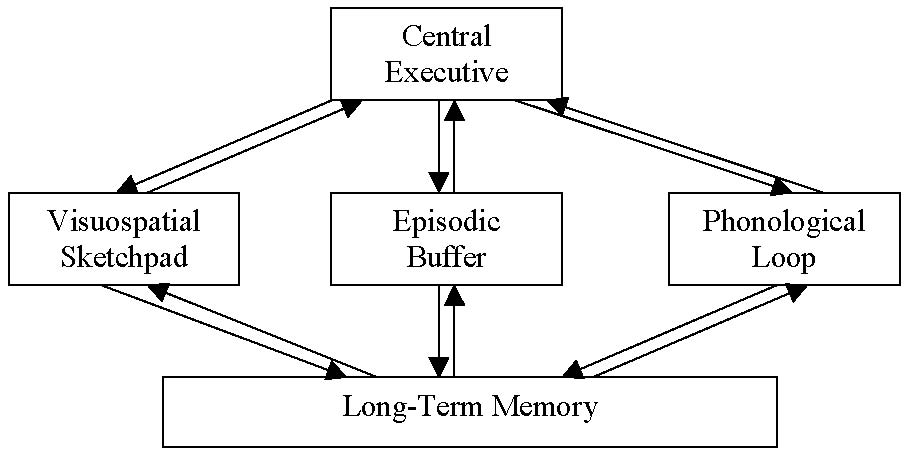
\includegraphics[width=0.45\linewidth]{figure/Baddeley_model} 

}

\caption{Working Memory Model created by Baddeley (left) and Information Processing Model created by Atkinson and Shiffrin (right)}\label{fig:unnamed-chunk-4-1}
\end{figure}
\begin{figure}

{\centering 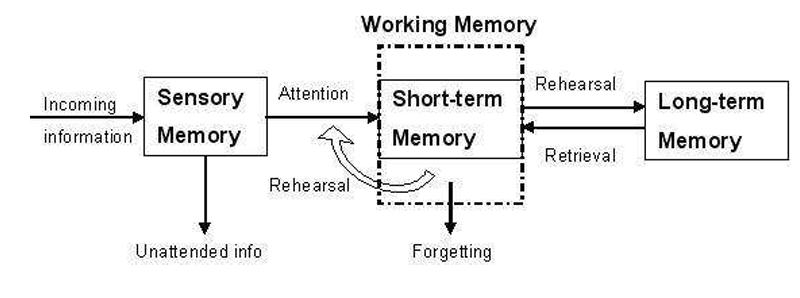
\includegraphics[width=0.45\linewidth]{figure/info_model} 

}

\caption{Working Memory Model created by Baddeley (left) and Information Processing Model created by Atkinson and Shiffrin (right)}\label{fig:unnamed-chunk-4-2}
\end{figure}

Visual and spatial information is processed and temporarily stored in the visuospatial sketchpad when individuals view statistical graphics.
The central executive component facilitates the interpretation and analysis of the presented data by directing attention to pertinent aspects of the graphic.
Utilizing working memory resources effectively can aid in comprehending and remembering the statistical information conveyed by the graphics.

Together, Baddeley's model of working memory provided a comprehensive framework for studying memory and cognition.
They contributed to the understanding of how information is processed, encoded, stored, and retrieved in human memory systems, laying the groundwork for subsequent research and theories in cognitive psychology.

\hypertarget{ensemble-perception}{%
\section{Ensemble Perception}\label{ensemble-perception}}

Ensemble perception is the cognitive ability to quickly derive summary statistics from sets of similar items (Chong \& Treisman, 2003).
This component of visual cognition enables the visual system to summarize and describe collections of comparable objects or features effectively.
This capability is often activated at a glance and is crucial for making sense of complex visual scenes.

David Whitney's fundamental review outlines the core principles of ensemble perception, emphasizing the extraction of summary statistical information from groups of similar objects (Whitney, Haberman, \& Sweeny, 2014) and (Dakin \& Watt, 1997).
Ensemble perception pertains to the capacity of the human visual system to efficiently and swiftly extract statistical data from a collection of items or objects, as opposed to separately processing each item.
The application of ensemble perception can be observed through the utilization of Gestalt principles of visual perception, including proximity (referring to the nearness of objects), similarity (pertaining to similar appearance), and closure (denoting the completion of shapes).
These concepts facilitate the perception of patterns and groups in visual scenes without necessitating a detailed examination of each individual piece.

Huberman et al.~further discussed that individual differences exist in ensemble perception capabilities, indicating the presence of multiple, independent levels of ensemble representation (J. Haberman, Brady, \& Alvarez, 2015).\\
Recent studies have expanded on these principles.\\
Khayat et al.'s work explores how ensemble perception can create a unified perception from groups of similar objects and also delves into the implicit perception and memory of set statistics (Khayat, Ahissar, \& Hochstein, 2023) and (Khayat, Fusi, \& Hochstein, 2021).
Examples of perception and memory of set statistics in visual information can best be described when you look at a field of flowers with various colors.
Your perception quickly summarizes the set statistics of color, such as the overall color distribution, or in a crowd of people, your perception helps you group individuals into categories based on shared characteristics like clothing color, height, or age.
In brief, the cognitive processes of perceiving and remembering statistical information in visual stimuli are crucial for efficiently comprehending and retaining the statistical characteristics of visual scenes and objects.
These mechanisms play a significant role in enhancing our comprehension and analysis of the visual environment.

The study ``Perceptual History Biases in Serial Ensemble Representation'' by Khayat et al.~focuses on ensemble perception, explicitly examining how past visual experiences influence the perception of current visual ensembles.\\
The study investigates the serial dependence of ensemble perception when each ensemble set is presented simultaneously but spatially distributed over the screen.\\
This suggests that the objects and our prior experiences with similar ensembles impact how we perceive groups of similar objects (Khayat et al., 2023).

This adds a layer of complexity to the understanding of ensemble perception, which is generally considered the visual system's ability to summarize groups of similar objects into a unified perception efficiently.

The study ``Perceiving ensemble statistics of novel image sets'' by Khayat et al.~focuses on how the human visual system perceives summary statistics of sets of stimulus elements.\\
The study is particularly interested in how we perceive novel image sets and hypothesizes that our capacity to summarize statistical data from these sets affects how well we can comprehend and interpret new visual information (Khayat et al., 2021).
This research contributes to the broader field of ensemble perception, which explores how the visual system can efficiently represent groups of similar objects as a unified perception.\\
The study implies that not only can the visual system quickly grasp the ``gist'' or essence of familiar visual ensembles, but it can also do so for novel sets of images.\\
This ability to quickly summarize statistical information from new visual stimuli could be a fundamental feature of human perception (Khayat \& Hochstein, 2018).\\
Other research has investigated the role of ensemble perception in both high- and low-level visual information, such as emotion and brightness, and how it can even operate when scene information is incomplete (Chakrabarty \& Wada, 2020) and (J. M. Haberman \& Ulrich, 2019).

Furthermore, ensemble perception is not just a specialized function but a pervasive aspect of visual perception.\\
It has been discussed holistically to engage a general audience and has been shown to condense redundant information into summary statistical representations (Corbett, Utochkin, \& Hochstein, 2023) and (Whitney \& Manassi, 2022).\\
Stable ensemble representations have been found to facilitate visual search, even when they are not predictive of a target location (Utochkin, Choi, \& Chong, 2023).
The study focuses on a coding model that emphasizes the crucial role of the ``pooling layer'' in ensemble perception.

\hypertarget{ensemble-visualization}{%
\subsection{Ensemble Visualization}\label{ensemble-visualization}}

Ensemble visualization refers to the graphical representation of ensemble data, which typically consists of multiple related datasets.
It aims to provide a comprehensive view that allows for rapidly extracting visual statistics and insights about distributed information.\\
Ensemble visualization techniques can vary, including Ensemble Surface Slicing (ESS) to visualize regions of similarity and difference among surfaces and statistical visualization techniques to identify areas of interest quickly (Alabi et al., 2012) and (Potter et al., 2009).\\
The aim is to provide a comprehensive view that allows for the rapid extraction of visual statistics and insights about distributed information.\\
By combining various statistical visualization techniques, Potter presents the Ensemble-Vis framework in his paper as a way for scientists to identify areas of interest quickly, (Potter et al., 2009).
The paper's thorough methodology, which combines various statistical visualization techniques to build a more helpful ensemble visualization framework, makes it noteworthy.
This framework has been referenced by many other studies, leading to the development of new visualization methods.

By exploring the effects of ensemble and summary displays on data interpretation, Padilla's research adds valuable insights to the field, (Padilla, Ruginski, \& Creem-Regehr, 2017).
Padilla investigates how ensemble displays, which plot multiple data points on the same Cartesian coordinate plane, affect the viewer's understanding and interpretation of the data.
The paper contributes to the theory by examining the cognitive aspects of ensemble visualization.
However, a counterexample to the effectiveness of ensemble displays can be observed when the data points are highly overlapping and densely packed, leading to visual clutter and difficulty distinguishing individual data points.
In such cases, ensemble displays may hinder the viewer's understanding and interpretation of the data rather than enhance it.
This highlights the importance of considering the specific characteristics of the presented data when deciding whether to use ensemble displays.
Additionally, summary displays, which provide an overview of the data, can be a helpful alternative in situations where ensemble displays may be less effective.
Summary displays condense the data into crucial statistics or visual representations, allowing for more straightforward interpretation and analysis, especially when dealing with complex or dense datasets.
Further research is needed to explore the optimal conditions for ensemble and summary displays to maximize their effectiveness in data interpretation.

\hypertarget{multidimensional-ensembles}{%
\subsection{Multidimensional Ensembles}\label{multidimensional-ensembles}}

Initial research on ensemble perception primarily focused on one-dimensional ensembles, where summary statistics are extracted from a single feature or dimension (J. Haberman et al., 2015).
For example, in a study on facial expression perception, participants were presented with an ensemble of faces displaying different emotions.
In this case, the pooling layer would analyze the overall emotional expression of the ensemble, summarizing the various individual facial expressions into one general emotion perception.
This model allows researchers to understand how humans perceive and interpret complex emotional expressions more systematically.
However, as Maule and Franklin note, real-world scenes often consist of complex, multidimensional attributes, and research has gradually shifted towards understanding how the human visual system processes these more intricate ensembles (Maule \& Franklin, 2015).
Research on multidimensional ensembles has explored how people simultaneously perceive summary statistics across multiple attributes, such as size and color.

Darkin and Watt were among the first to explore how orientation statistics are computed from visual textures, extending the concept of ensemble perception into a multidimensional setting, (Dakin \& Watt, 1997).
Haberman et al.~expanded this research by showing that individual differences exist in ensemble perception capabilities, suggesting multiple, independent levels of ensemble representation exist, (J. Haberman et al., 2015).
The existing literature on multidimensional ensembles in visual information covers various topics, from neuroscience to data visualization.\\
For instance, studies have explored the role of neuronal ensembles in controlling visually guided behavior and their influence on visual working memory (Carrillo-Reid, Han, Yang, Akrouh, \& Yuste, 2019).
Research has also delved into the use of aggregated plots for multidimensional visual analysis, although these don't explicitly mention ensembles (Fofonov \& Linsen, 2018).\\
Fast ensemble representations have been investigated to understand high-level perceptual impressions based on visual information (Leib, Kosovicheva, \& Whitney, 2016).

Additionally, the aesthetic complexity of visual information has been quantified using information theory, offering a potential framework for ensemble-based representations (Karjus, Solà, Ohm, Ahnert, \& Schich, 2023).
But a detailed example of why you shouldn't use aggregated plots for multidimensional visual analysis is when the individual data points in the ensemble show significant differences. Data aggregation may obscure important patterns in such scenarios and lead to misleading interpretations.
Further, ensembles may fail to capture the fine-grained details and nuances present in the individual plots, compromising the overall accuracy and precision of the analysis.
The long-term stability of neuronal ensembles in the visual cortex has been studied, shedding light on their potential role in visual perception (Pérez-Ortega, Alejandre-Garcı́a, \& Yuste, 2021).
Ensemble visualization techniques, particularly in computer simulations, have also been reviewed (Afzal et al., 2019).
Lastly, the structure of neural networks has been shown to affect working memory, which could have implications for visual ensembles (Leavitt, Pieper, Sachs, \& Martinez-Trujillo, 2017).

\hypertarget{ref-labels}{%
\chapter{Does Color Help?: Multidimensional Ensembles in Bland-Altman Plots: An Exploration}\label{ref-labels}}

\hypertarget{introduction-3}{%
\section{Introduction:}\label{introduction-3}}

``How can multidimensional ensembles be effectively incorporated into Bland-Altman plots to enhance the accuracy and comprehensibility of assessing agreement between multiple measurement techniques?''
This research question explores the theoretical and practical implications of incorporating ensemble perception and multidimensional data into Bland-Altman plots, traditionally used for comparing two measurement methods.
By doing so, the research seeks to advance the utility and interpretability of these plots in complex, real-world scenarios where multiple dimensions are often at play.
The interpretation of Bland-Altman plots is conventionally one-dimensional, focusing primarily on the mean difference and limits of agreement (Bland \& Altman, 1986).
However, in real-world applications, the measurements under consideration often contain multiple dimensions that could contribute to interpreting the agreement or disagreement between two techniques (Chong \& Treisman, 2003).
A detailed counterexample of the utility and interpretability of Bland-Altman plots in complex, real-world scenarios can be seen where two techniques are being compared for measuring blood pressure.
The Bland-Altman plot may show good agreement between the mean difference and the limits of agreement, suggesting high concordance.
However, when considering additional dimensions such as accuracy and precision in different subgroups (e.g., age, gender), it could reveal significant discrepancies and limitations in the interpretation of Ensemble coding, a perceptual mechanism that provides a statistical summary of a visual scene, offers a promising solution by facilitating the rapid extraction of variability information (Alvarez, 2011).
The theory of ensemble perception offers a framework for understanding how these multiple dimensions could be processed simultaneously (J. Haberman et al., 2015) and (Whitney et al., 2014).

\hypertarget{ensemble-perception-1}{%
\subsection{Ensemble Perception}\label{ensemble-perception-1}}

Ensemble perception is the cognitive ability to quickly derive summary statistics from sets of similar items (Chong \& Treisman, 2003).
This component of visual cognition enables the visual system to summarize and describe collections of comparable objects or features effectively.
This capability is often activated at a glance and is crucial for making sense of complex visual scenes.

David Whitney's fundamental review outlines the core principles of ensemble perception, emphasizing the extraction of summary statistical information from groups of similar objects (Whitney et al., 2014) and (Dakin \& Watt, 1997).\\
(J. Haberman et al., 2015) further discussed that individual differences exist in ensemble perception capabilities, indicating the presence of multiple, independent levels of ensemble representation.\\
Recent studies have expanded on these principles.\\
Khayat et al.'s work explores how ensemble perception can create a unified perception from groups of similar objects and also delves into the implicit perception and memory of set statistics (Khayat et al., 2023) and (Khayat et al., 2021).\\
The study ``Perceptual History Biases in Serial Ensemble Representation'' by Khayat et al.~focuses on ensemble perception, explicitly examining how past visual experiences influence the perception of current visual ensembles.\\
The study investigates the serial dependence of ensemble perception when each ensemble set is presented simultaneously but spatially distributed over the screen.\\
This suggests that the objects and our prior experiences with similar ensembles impact how we perceive groups of similar objects (Khayat et al., 2023).
This adds a layer of complexity to the understanding of ensemble perception, which is generally considered the visual system's ability to summarize groups of similar objects into a unified perception efficiently.\\
The study ``Perceiving ensemble statistics of novel image sets'' by Khayat et al.~focuses on how the human visual system perceives summary statistics of sets of stimulus elements.\\
The study is particularly interested in how we perceive novel image sets and hypothesizes that our capacity to summarize statistical data from these sets affects how well we can comprehend and interpret new visual information (Khayat et al., 2021).
This research contributes to the broader field of ensemble perception, which explores how the visual system can efficiently represent groups of similar objects as a unified perception.\\
The study implies that not only can the visual system quickly grasp the ``gist'' or essence of familiar visual ensembles, but it can also do so for novel sets of images.\\
This ability to quickly summarize statistical information from new visual stimuli could be a fundamental feature of human perception (Khayat \& Hochstein, 2018).\\
Other research has investigated the role of ensemble perception in both high- and low-level visual information, such as emotion and brightness, and how it can even operate when scene information is incomplete (Chakrabarty \& Wada, 2020) and (J. M. Haberman \& Ulrich, 2019).

Furthermore, ensemble perception is not just a specialized function but a pervasive aspect of visual perception.\\
It has been discussed holistically to engage a general audience and has been shown to condense redundant information into summary statistical representations (Corbett et al., 2023) and (Whitney \& Manassi, 2022).\\
Lastly, stable ensemble representations have been found to facilitate visual search, even when they are not predictive of a target location (Utochkin et al., 2023).
The study focuses on a coding model that emphasizes the crucial role of the ``pooling layer'' in ensemble perception.\\
Ensemble perception refers to the ability of the visual system to summarize information from a group of similar objects.
The ``pooling layer'' in the model likely serves as a computational mechanism for aggregating or summarizing this information, potentially providing insights into how the brain processes complex visual scenes.
The study aims to provide a more structured understanding of ensemble perception by introducing a model highlighting the importance of a specific computational layer, known as the ``pooling layer,'' in summarizing visual information.

\hypertarget{multidimensional-ensembles-1}{%
\subsection{Multidimensional Ensembles}\label{multidimensional-ensembles-1}}

Initial research on ensemble perception primarily focused on one-dimensional ensembles, where summary statistics are extracted from a single feature or dimension (J. Haberman et al., 2015).
For example, in a study on facial expression perception, participants were presented with an ensemble of faces displaying different emotions.
In this case, the pooling layer would analyze the overall emotional expression of the ensemble, summarizing the various individual facial expressions into one general emotion perception.
This model allows researchers to understand how humans perceive and interpret complex emotional expressions more systematically.
However, as (Maule \& Franklin, 2015) notes, real-world scenes often consist of complex, multidimensional attributes, and research has gradually shifted towards understanding how the human visual system processes these more intricate ensembles.
Research on multidimensional ensembles has explored how people simultaneously perceive summary statistics across multiple attributes, such as size and color.

(Dakin \& Watt, 1997) were among the first to explore how orientation statistics are computed from visual textures, extending the concept of ensemble perception into a multidimensional setting.
(J. Haberman et al., 2015) expanded this research by showing that individual differences exist in ensemble perception capabilities, suggesting multiple, independent levels of ensemble representation exist.
The existing literature on multidimensional ensembles in visual information covers various topics, from neuroscience to data visualization.\\
For instance, studies have explored the role of neuronal ensembles in controlling visually guided behavior and their influence on visual working memory (Carrillo-Reid et al., 2019).
Research has also delved into the use of aggregated plots for multidimensional visual analysis, although these don't explicitly mention ensembles (Fofonov \& Linsen, 2018).\\
Fast ensemble representations have been investigated to understand high-level perceptual impressions based on visual information (Leib et al., 2016).

Additionally, the aesthetic complexity of visual information has been quantified using information theory, offering a potential framework for ensemble-based representations (Karjus et al., 2023).
But a detailed example of why you shouldn't use aggregated plots for multidimensional visual analysis is when the individual data points in the ensemble show significant differences. Data aggregation may obscure important patterns in such scenarios and lead to misleading interpretations.
Further, ensembles may fail to capture the fine-grained details and nuances present in the individual plots, compromising the overall accuracy and precision of the analysis.
The long-term stability of neuronal ensembles in the visual cortex has been studied, shedding light on their potential role in visual perception (Pérez-Ortega et al., 2021).
Ensemble visualization techniques, particularly in computer simulations, have also been reviewed (Afzal et al., 2019).
Lastly, the structure of neural networks has been shown to affect working memory, which could have implications for visual ensembles (Leavitt et al., 2017).

\hypertarget{bland-altman-plots}{%
\subsection{Bland-Altman Plots}\label{bland-altman-plots}}

The study of multidimensional ensembles has seen applications in the field of data visualization.
(Szafir, 2017) showed that understanding color differences could improve the design of visualizations that require the viewer to integrate multiple pieces of information.
This work suggested that effective visualization tools could be designed by leveraging the human ability to process multidimensional ensembles rapidly.

Bland-Altman Plots are widely used in clinical research for assessing the agreement between two measurement techniques by plotting the differences against the means (Bland \& Altman, 1986).
They offer a straightforward representation of data, making them a popular choice for visualizing measurement bias.
However, the plots are conventionally one-dimensional, primarily focusing on mean differences and limits of agreement.

\hypertarget{the-intersection-of-multidimensional-ensembles-and-bland-altman-plots}{%
\subsection{The intersection of Multidimensional Ensembles and Bland-Altman Plots}\label{the-intersection-of-multidimensional-ensembles-and-bland-altman-plots}}

The application of multidimensional ensembles in Bland-Altman Plots could potentially offer a more nuanced understanding of data.
For example, integrating color coding to indicate standard deviation and shape variations to indicate skewness could offer additional layers of information in a single plot (Szafir, 2017).
Such an approach could leverage our innate abilities in ensemble perception to offer a more comprehensive assessment of agreement between multiple sets of measurement techniques (Szafir, Haroz, Gleicher, \& Franconeri, 2016).

\hypertarget{gaps-in-research}{%
\subsection{Gaps in Research}\label{gaps-in-research}}

While the fields of ensemble perception and data visualization have seen significant growth, there is a lack of research focusing on the application of ensemble perception, particularly multidimensional ensembles, in Bland-Altman Plots.
This gap points to the need for empirical studies designed to validate theoretical frameworks and to assess the practical utility of incorporating multidimensional ensembles into Bland-Altman Plots.

\hypertarget{methods}{%
\section{Methods:}\label{methods}}

Ensemble perception involves the rapid and often unconscious extraction of summary statistics from a set of similar items (Chong \& Treisman, 2003), (Whitney et al., 2014).
In the context of multidimensional ensembles, this would refer to the simultaneous extraction of various features such as mean, variance, and other statistical attributes across multiple dimensions (Maule \& Franklin, 2015), (J. Haberman et al., 2015).
Understanding this concept will provide a unique way to interpret Bland-Altman plots that contain data from multiple dimensions.

Traditionally, Bland-Altman plots present the difference between two sets of measurements against their mean, providing a graphical representation of agreement or bias.
However, this one-dimensional representation might not capture the full complexity of real-world data, where measurements can often be multidimensional (Dakin \& Watt, 1997).
Given the human brain's ability to rapidly process multidimensional ensemble statistics (J. Haberman et al., 2015), incorporating this aspect into Bland-Altman plots might yield a more nuanced interpretation (Bauer, 2009), (Szafir et al., 2016).

One way to incorporate multidimensionality into Bland-Altman plots is by adding layers that represent different statistical attributes.
For example, varying shades of color could indicate the standard deviation within each plotted point, and shape variations could indicate another dimension such as skewness or kurtosis (Szafir, 2017).
This model would require human observers to simultaneously extract multiple summary statistics, leveraging the brain's capabilities in ensemble perception (Chong \& Treisman, 2003).

In this proposed study, we utilize color coding to represent varying levels of variability in Bland-Altman plots.
To ensure the universal interpretability of the plots (Ware, 2012), the color palette will be selected with care, taking into account potential issues such as color blindness.

For this study, two Bland-Altman plots will be generated.
A traditional plot without color-coding and a plot using the color-coding technique we propose.
Both plots will be presented to a group of participants that includes both experts and non-experts in data interpretation and statistics.
The participants will be required to interpret the plots and complete a questionnaire to assess their comprehension and speed of interpretation.

For a layer of interactivity in our study, we will generate interactive Bland-Altman plots incorporating ensemble coding of variability through color gradations.
Interactivity will be implemented via D3, providing detailed information about each data point when hovered over, as well as zoom features allowing users to zero in on areas of interest.

\hypertarget{design-of-the-user-studies}{%
\subsection{Design of the User Studies}\label{design-of-the-user-studies}}

User studies will be designed to assess the effectiveness of the interactive Bland-Altman plots in conveying information about the variability of data points.
The studies will consist of two parts:

\textbf{Task-based Evaluation:} Participants will be given a set of tasks to complete using both the interactive color-coded Bland-Altman plot and a traditional static Bland-Altman plot.
Tasks will involve identifying specific data points, interpreting data variability, and answering questions about the overall data trend.
Metrics such as task completion time, success rate, and error rate will be recorded (Rubin \& Chisnell, 2008).

\textbf{Subjective Evaluation:} After completing the tasks, participants will be asked to fill out a questionnaire assessing their user experience.
The questionnaire will include items related to the perceived ease of use, satisfaction, and preference between the traditional and interactive color-coded Bland-Altman plots.

\hypertarget{discussion-1}{%
\section{Discussion:}\label{discussion-1}}

We anticipate that the application of ensemble coding for variability will aid in the comprehension of Bland-Altman plots.
Based on ensemble coding principles, the color-coded plot should enable faster and more accurate interpretation of data variability (J. Haberman \& Whitney, 2012).
This method has the potential to enhance the interpretability and utility of these graphs, making them accessible to a broader audience and facilitating more efficient data communication.

\hypertarget{conclusion}{%
\chapter*{Conclusion}\label{conclusion}}
\addcontentsline{toc}{chapter}{Conclusion}

If we don't want Conclusion to have a chapter number next to it, we can add the \texttt{\{-\}} attribute.

\textbf{More info}

And here's some other random info: the first paragraph after a chapter title or section head \emph{shouldn't be} indented, because indents are to tell the reader that you're starting a new paragraph. Since that's obvious after a chapter or section title, proper typesetting doesn't add an indent there.

\appendix

\hypertarget{the-first-appendix}{%
\chapter{The First Appendix}\label{the-first-appendix}}

This first appendix includes all of the R chunks of code that were hidden throughout the document (using the \texttt{include\ =\ FALSE} chunk tag) to help with readibility and/or setup.

\textbf{In the main Rmd file}

\begin{Shaded}
\begin{Highlighting}[]
\FunctionTok{library}\NormalTok{(knitr)}
\FunctionTok{library}\NormalTok{(palmerpenguins)}
\FunctionTok{library}\NormalTok{(tidyverse)}
\FunctionTok{library}\NormalTok{(nycflights13)}
\FunctionTok{data}\NormalTok{(flights)}

\FunctionTok{library}\NormalTok{(ggpcp)}
\FunctionTok{library}\NormalTok{(ggplot2)}
\FunctionTok{library}\NormalTok{(dplyr)}
\FunctionTok{data}\NormalTok{(nasa)}

\FunctionTok{library}\NormalTok{(scales)}
\FunctionTok{library}\NormalTok{(datasets)}
\FunctionTok{data}\NormalTok{(}\StringTok{"ChickWeight"}\NormalTok{)}
\FunctionTok{library}\NormalTok{(formatR)}
\end{Highlighting}
\end{Shaded}

\textbf{In Chapter \ref{ref-labels}:}

\hypertarget{the-second-appendix-for-fun}{%
\chapter{The Second Appendix, for Fun}\label{the-second-appendix-for-fun}}

\hypertarget{colophon}{%
\chapter*{Colophon}\label{colophon}}
\addcontentsline{toc}{chapter}{Colophon}

This document is set in \href{https://github.com/georgd/EB-Garamond}{EB Garamond}, \href{https://github.com/adobe-fonts/source-code-pro/}{Source Code Pro} and \href{http://www.latofonts.com/lato-free-fonts/}{Lato}. The body text is set at 11pt with \(\familydefault\).

It was written in R Markdown and \(\LaTeX\), and rendered into PDF using \href{https://github.com/benmarwick/huskydown}{huskydown} and \href{https://github.com/rstudio/bookdown}{bookdown}.

This document was typeset using the XeTeX typesetting system, and the \href{http://staff.washington.edu/fox/tex/}{University of Washington Thesis class} class created by Jim Fox. Under the hood, the \href{https://github.com/UWIT-IAM/UWThesis}{University of Washington Thesis LaTeX template} is used to ensure that documents conform precisely to submission standards. Other elements of the document formatting source code have been taken from the \href{https://github.com/stevenpollack/ucbthesis}{Latex, Knitr, and RMarkdown templates for UC Berkeley's graduate thesis}, and \href{https://github.com/suchow/Dissertate}{Dissertate: a LaTeX dissertation template to support the production and typesetting of a PhD dissertation at Harvard, Princeton, and NYU}

The source files for this thesis, along with all the data files, have been organised into an R package, xxx, which is available at \url{https://github.com/xxx/xxx}. A hard copy of the thesis can be found in the University of Washington library.

This version of the thesis was generated on 2024-07-29 14:53:30.337635. The repository is currently at this commit:

The computational environment that was used to generate this version is as follows:

\begin{verbatim}
## - Session info -------------------------------------------
##  setting  value
##  version  R version 4.4.1 (2024-06-14)
##  os       Debian GNU/Linux 12 (bookworm)
##  system   x86_64, linux-gnu
##  ui       X11
##  language (EN)
##  collate  en_US.UTF-8
##  ctype    en_US.UTF-8
##  tz       America/Chicago
##  date     2024-07-29
##  pandoc   3.1.1 @ /usr/lib/rstudio/resources/app/bin/quarto/bin/tools/ (via rmarkdown)
## 
## - Packages -----------------------------------------------
##  package        * version date (UTC) lib source
##  assertthat       0.2.1   2019-03-21 [2] CRAN (R 4.4.0)
##  bookdown         0.40    2024-07-02 [2] CRAN (R 4.4.1)
##  cachem           1.1.0   2024-05-16 [2] CRAN (R 4.4.1)
##  cli              3.6.3   2024-06-21 [2] CRAN (R 4.4.1)
##  colorspace       2.1-1   2024-07-26 [2] CRAN (R 4.4.1)
##  data.table       1.15.4  2024-03-30 [2] CRAN (R 4.4.0)
##  devtools         2.4.5   2022-10-11 [2] CRAN (R 4.4.0)
##  digest           0.6.36  2024-06-23 [2] CRAN (R 4.4.1)
##  dplyr          * 1.1.4   2023-11-17 [2] CRAN (R 4.4.0)
##  ellipsis         0.3.2   2021-04-29 [2] CRAN (R 4.3.1)
##  evaluate         0.24.0  2024-06-10 [2] CRAN (R 4.4.1)
##  fansi            1.0.6   2023-12-08 [2] CRAN (R 4.4.0)
##  farver           2.1.2   2024-05-13 [2] CRAN (R 4.4.1)
##  fastmap          1.2.0   2024-05-15 [2] CRAN (R 4.4.1)
##  forcats        * 1.0.0   2023-01-29 [2] CRAN (R 4.4.0)
##  formatR        * 1.14    2023-01-17 [2] CRAN (R 4.4.0)
##  fs               1.6.4   2024-04-25 [2] CRAN (R 4.4.0)
##  generics         0.1.3   2022-07-05 [2] CRAN (R 4.3.1)
##  ggpcp          * 0.2.0   2024-07-26 [2] Github (heike/ggpcp@bdb2fea)
##  ggplot2        * 3.5.1   2024-04-23 [2] CRAN (R 4.4.0)
##  glue             1.7.0   2024-01-09 [2] CRAN (R 4.4.0)
##  gtable           0.3.5   2024-04-22 [2] CRAN (R 4.4.0)
##  hms              1.1.3   2023-03-21 [2] CRAN (R 4.3.1)
##  htmltools        0.5.8.1 2024-04-04 [2] CRAN (R 4.4.0)
##  htmlwidgets      1.6.4   2023-12-06 [2] CRAN (R 4.4.0)
##  httpuv           1.6.15  2024-03-26 [2] CRAN (R 4.4.0)
##  httr             1.4.7   2023-08-15 [2] CRAN (R 4.4.0)
##  jsonlite         1.8.8   2023-12-04 [2] CRAN (R 4.4.0)
##  knitr          * 1.48    2024-07-07 [2] CRAN (R 4.4.1)
##  labeling         0.4.3   2023-08-29 [2] CRAN (R 4.3.1)
##  later            1.3.2   2023-12-06 [2] CRAN (R 4.3.2)
##  lazyeval         0.2.2   2019-03-15 [2] CRAN (R 4.4.0)
##  lifecycle        1.0.4   2023-11-07 [2] CRAN (R 4.3.2)
##  lubridate      * 1.9.3   2023-09-27 [2] CRAN (R 4.4.0)
##  magrittr         2.0.3   2022-03-30 [2] CRAN (R 4.4.0)
##  memoise          2.0.1   2021-11-26 [2] CRAN (R 4.3.1)
##  mime             0.12    2021-09-28 [2] CRAN (R 4.4.0)
##  miniUI           0.1.1.1 2018-05-18 [2] CRAN (R 4.4.0)
##  munsell          0.5.1   2024-04-01 [2] CRAN (R 4.4.0)
##  nycflights13   * 1.0.2   2021-04-12 [2] CRAN (R 4.4.0)
##  palmerpenguins * 0.1.1   2022-08-15 [2] CRAN (R 4.4.0)
##  pillar           1.9.0   2023-03-22 [2] CRAN (R 4.4.0)
##  pkgbuild         1.4.4   2024-03-17 [2] CRAN (R 4.4.0)
##  pkgconfig        2.0.3   2019-09-22 [2] CRAN (R 4.3.1)
##  pkgload          1.4.0   2024-06-28 [2] CRAN (R 4.4.1)
##  plotly           4.10.4  2024-01-13 [2] CRAN (R 4.4.0)
##  profvis          0.3.8   2023-05-02 [2] CRAN (R 4.4.0)
##  promises         1.3.0   2024-04-05 [2] CRAN (R 4.4.0)
##  purrr          * 1.0.2   2023-08-10 [2] CRAN (R 4.4.0)
##  R6               2.5.1   2021-08-19 [2] CRAN (R 4.3.1)
##  RColorBrewer     1.1-3   2022-04-03 [2] CRAN (R 4.4.0)
##  Rcpp             1.0.13  2024-07-17 [2] CRAN (R 4.4.1)
##  readr          * 2.1.5   2024-01-10 [2] CRAN (R 4.4.0)
##  remotes          2.5.0   2024-03-17 [2] CRAN (R 4.4.0)
##  rlang            1.1.4   2024-06-04 [2] CRAN (R 4.4.1)
##  rmarkdown        2.27    2024-05-17 [2] CRAN (R 4.4.1)
##  rstudioapi       0.16.0  2024-03-24 [2] CRAN (R 4.4.0)
##  scales         * 1.3.0   2023-11-28 [2] CRAN (R 4.4.0)
##  sessioninfo      1.2.2   2021-12-06 [2] CRAN (R 4.3.2)
##  shiny            1.8.1.1 2024-04-02 [2] CRAN (R 4.4.0)
##  stringi          1.8.4   2024-05-06 [2] CRAN (R 4.4.0)
##  stringr        * 1.5.1   2023-11-14 [2] CRAN (R 4.4.0)
##  tibble         * 3.2.1   2023-03-20 [2] CRAN (R 4.4.0)
##  tidyr          * 1.3.1   2024-01-24 [2] CRAN (R 4.4.0)
##  tidyselect       1.2.1   2024-03-11 [2] CRAN (R 4.4.0)
##  tidyverse      * 2.0.0   2023-02-22 [2] CRAN (R 4.4.0)
##  timechange       0.3.0   2024-01-18 [2] CRAN (R 4.3.2)
##  tzdb             0.4.0   2023-05-12 [2] CRAN (R 4.3.1)
##  urlchecker       1.0.1   2021-11-30 [2] CRAN (R 4.3.2)
##  usethis          3.0.0   2024-07-29 [2] CRAN (R 4.4.1)
##  utf8             1.2.4   2023-10-22 [2] CRAN (R 4.3.2)
##  vctrs            0.6.5   2023-12-01 [2] CRAN (R 4.4.0)
##  viridisLite      0.4.2   2023-05-02 [2] CRAN (R 4.3.1)
##  withr            3.0.0   2024-01-16 [2] CRAN (R 4.4.0)
##  xfun             0.46    2024-07-18 [2] CRAN (R 4.4.1)
##  xtable           1.8-4   2019-04-21 [2] CRAN (R 4.4.0)
##  yaml             2.3.10  2024-07-26 [2] CRAN (R 4.4.1)
## 
##  [1] /home/susan/R/x86_64-pc-linux-gnu-library/4.4
##  [2] /usr/local/lib/R/site-library
##  [3] /usr/lib/R/site-library
##  [4] /usr/lib/R/library
## 
## ----------------------------------------------------------
\end{verbatim}

\backmatter

\hypertarget{references}{%
\chapter*{References}\label{references}}
\addcontentsline{toc}{chapter}{References}

\noindent

\setlength{\parindent}{-0.20in}
\setlength{\leftskip}{0.20in}
\setlength{\parskip}{8pt}

\hypertarget{general-introduction}{%
\chapter{General Introduction}\label{general-introduction}}

Statisticians use graphs in almost every stage of their work.
They create charts to summarize and explore new data and identify potential problems and opportunities.
Models are fit based on relationships between variables which are often identified visually.
We identify problems with those models based on residual plots and other visual diagnostics.
When our modeling work has been completed, we present our results to interested parties using visual displays, because non-statisticians often find it easier to understand data and models through an intuitive visual medium rather than through the mathematical formulae which underlie the statistical work.

Given the wide range of uses for graphs and visual data displays in statistical modeling, it is unsurprising that some graphs are more useful for specific applications, such as exploratory analysis, and are unsuitable for other applications, such as presenting to an outside group.
In addition, not all visual displays have equal perceptual value Aspillaga (1996).
The best graphics are designed to account for both the dataset and the intended audience's features.
Some design constraints stem from limitations of the human perceptual system and are common to most potential consumers of the visualization.
For example, the sine illusion affects anyone with binocular depth perception, and color recommendations are built around the specific characteristics of the human retina (VanderPlas \& Hofmann, 2015b).
Other design constraints are due to the audience's experience level and if they are used to working with data and understand specialized techniques (e.g., enough familiarity with principal component analysis such that a plot of factor loadings might be useful).
Do they understand specialized techniques such as principal component analysis to the point where a plot of factor loadings might be a useful visual display?
When we create visualizations for public consumption, we have to consider both perceptual factors and the target audience's domain knowledge.
This introduction presents previous research on constructing interactive and static visual displays for different audiences and the implications of this research when designing interactive data displays such as dashboards.

Most research in statistical graphics has been done on static graphics; usually, research also strips away all but the most essential contextual information, sacrificing external validity for statistical control.
As a result, it can be hard to generalize this research to practical applications, where the contextual information surrounding the data is critical and the chart does not just exist in a vacuum.

In the real world, however, conventions and familiarity often win out over best practice validated by perceptual experiments.
For example, in sports, many coaches desire printable diagrams containing all necessary and valuable information on a single page.
As data in sports becomes more prominent, extensive, and collected, this information must be refined.

Thus, in addition to the experimental evidence, we must consider the human element: how to introduce new graphical concepts to stakeholders, and the considerations involved in encouraging stakeholders to adopt these improved graphics.
Let us first consider the audience characteristics that affect the selection of graphics.
Then, we will engage with considerations based on the data to be displayed.
Finally, we will consider the interactions between the audience and the data: how graphics are tested, amended, and hopefully eventually adopted into common use.

\hypertarget{methodology---exploratory-data-analysis-eda}{%
\section{Methodology - Exploratory Data Analysis (EDA)}\label{methodology---exploratory-data-analysis-eda}}

John Tukey was the first to organize the collection and methods associated with philosophy into Exploratory Data Analysis (EDA).
Previous research by Tukey focused on graphics as a tool for exploratory analysis.
In ``Exploratory Data Analysis,'' Tukey wrote that graphics and charts often display data with more enhanced understanding than a table, (Tukey \& Wilk, 1966).
Tukey outlines detailed the types of different graphics and in which situations to utilize these graphics.
He was a strong advocate for the importance of EDA as a crucial first step in the data analysis process and emphasized the need for visualization and interactive techniques to understand patterns and relationships in data.

Tukey's Principles of EDA have become a cornerstone in the field of statistics and have been adopted by data professionals in various industries.
Tukey's principles have enabled data professionals to understand complex data sets better and make more informed decisions by emphasizing the importance of visual exploration, data characterization, and model critique.
In this way, Tukey's Principles have revolutionized our data analysis approach and~become the foundational framework for EDA.

Tukey's Principles in EDA:

\begin{enumerate}
\def\labelenumi{\arabic{enumi}.}
\item
  Graphical exploration, looking for patterns or displaying fit, the method demonstrates things about data that a single numeric metric does not understand.
  This has been useful in graphing the data before you develop summary statistics.
\item
  Describing the general patterns of the data.
  This step should be insensitive to outliers.
  In general, think about the types of resistant measures (i.e., median or mean).
  This step is making sure to determine data patterns.
\item
  The natural scale/state that the data are at their best.
  This will be the step at which the scale of data can be helpful for analysis.
  The reexpressing data to a new scale by taking the square root or logarithmic scale.
\item
  The mostly known parts of EDA but is done in the way of accessing fit of the data.
  This is taught in every statistics 101 class.
  The growth of machine learning and prediction methods have now used residuals more in the toolbox to assessing the best prediction models.
\end{enumerate}

\begin{center}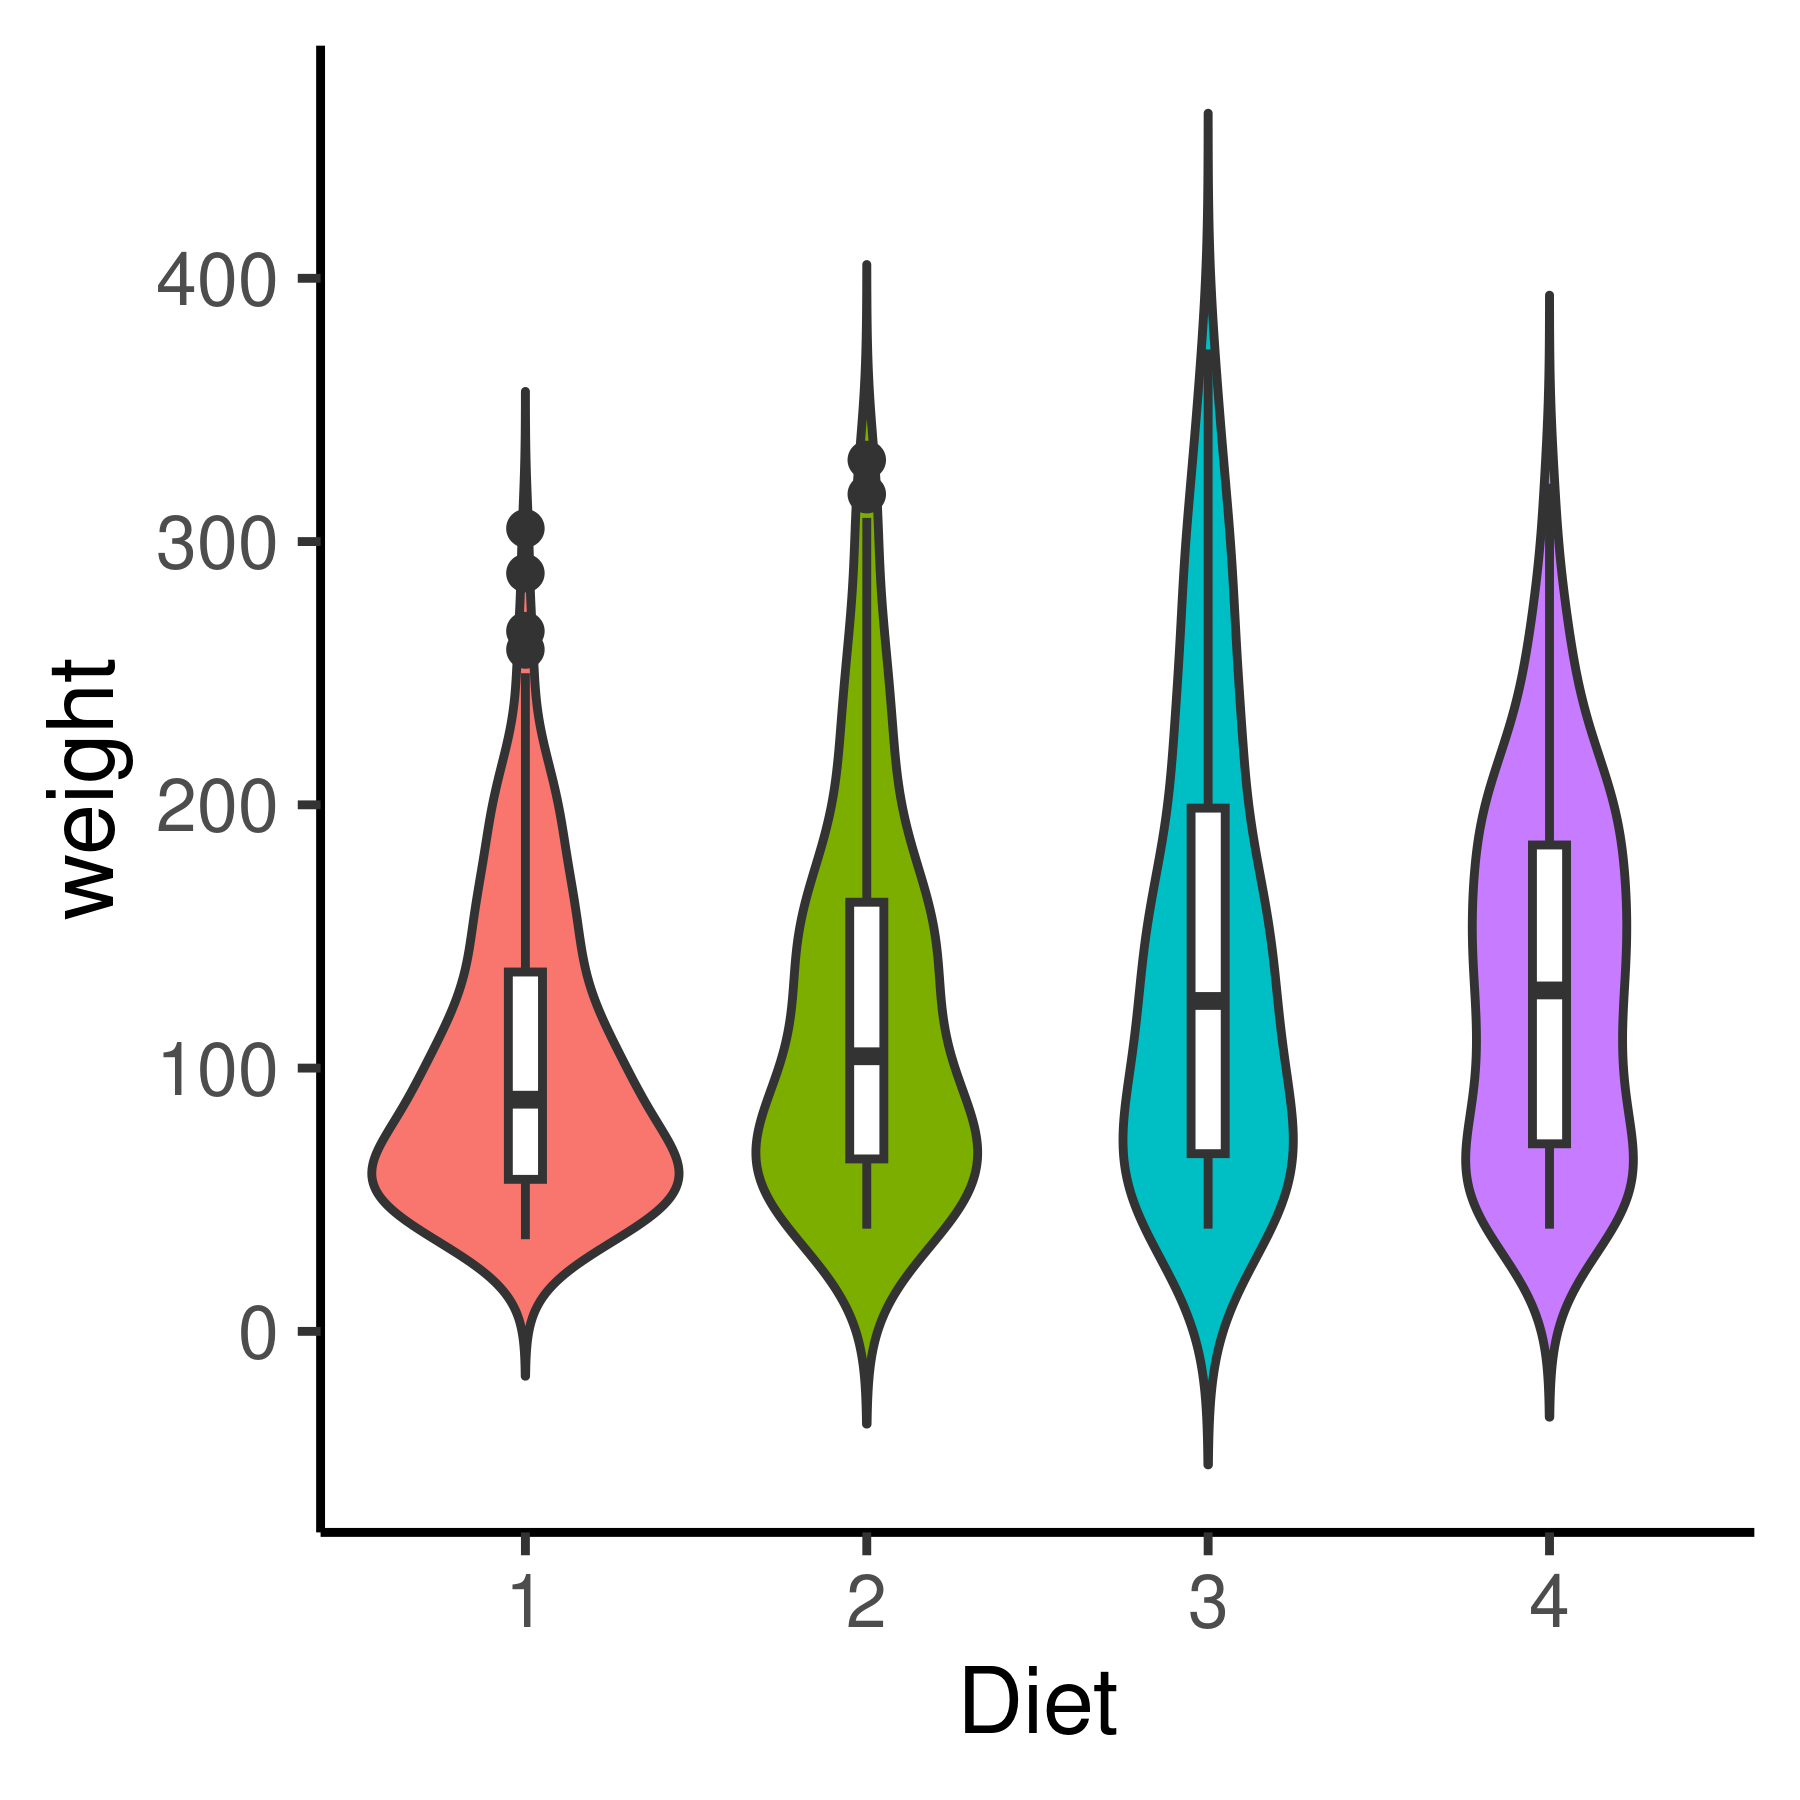
\includegraphics[width=.49\linewidth]{thesis_files/figure-latex/violin_plot-1} \end{center}

\begin{center}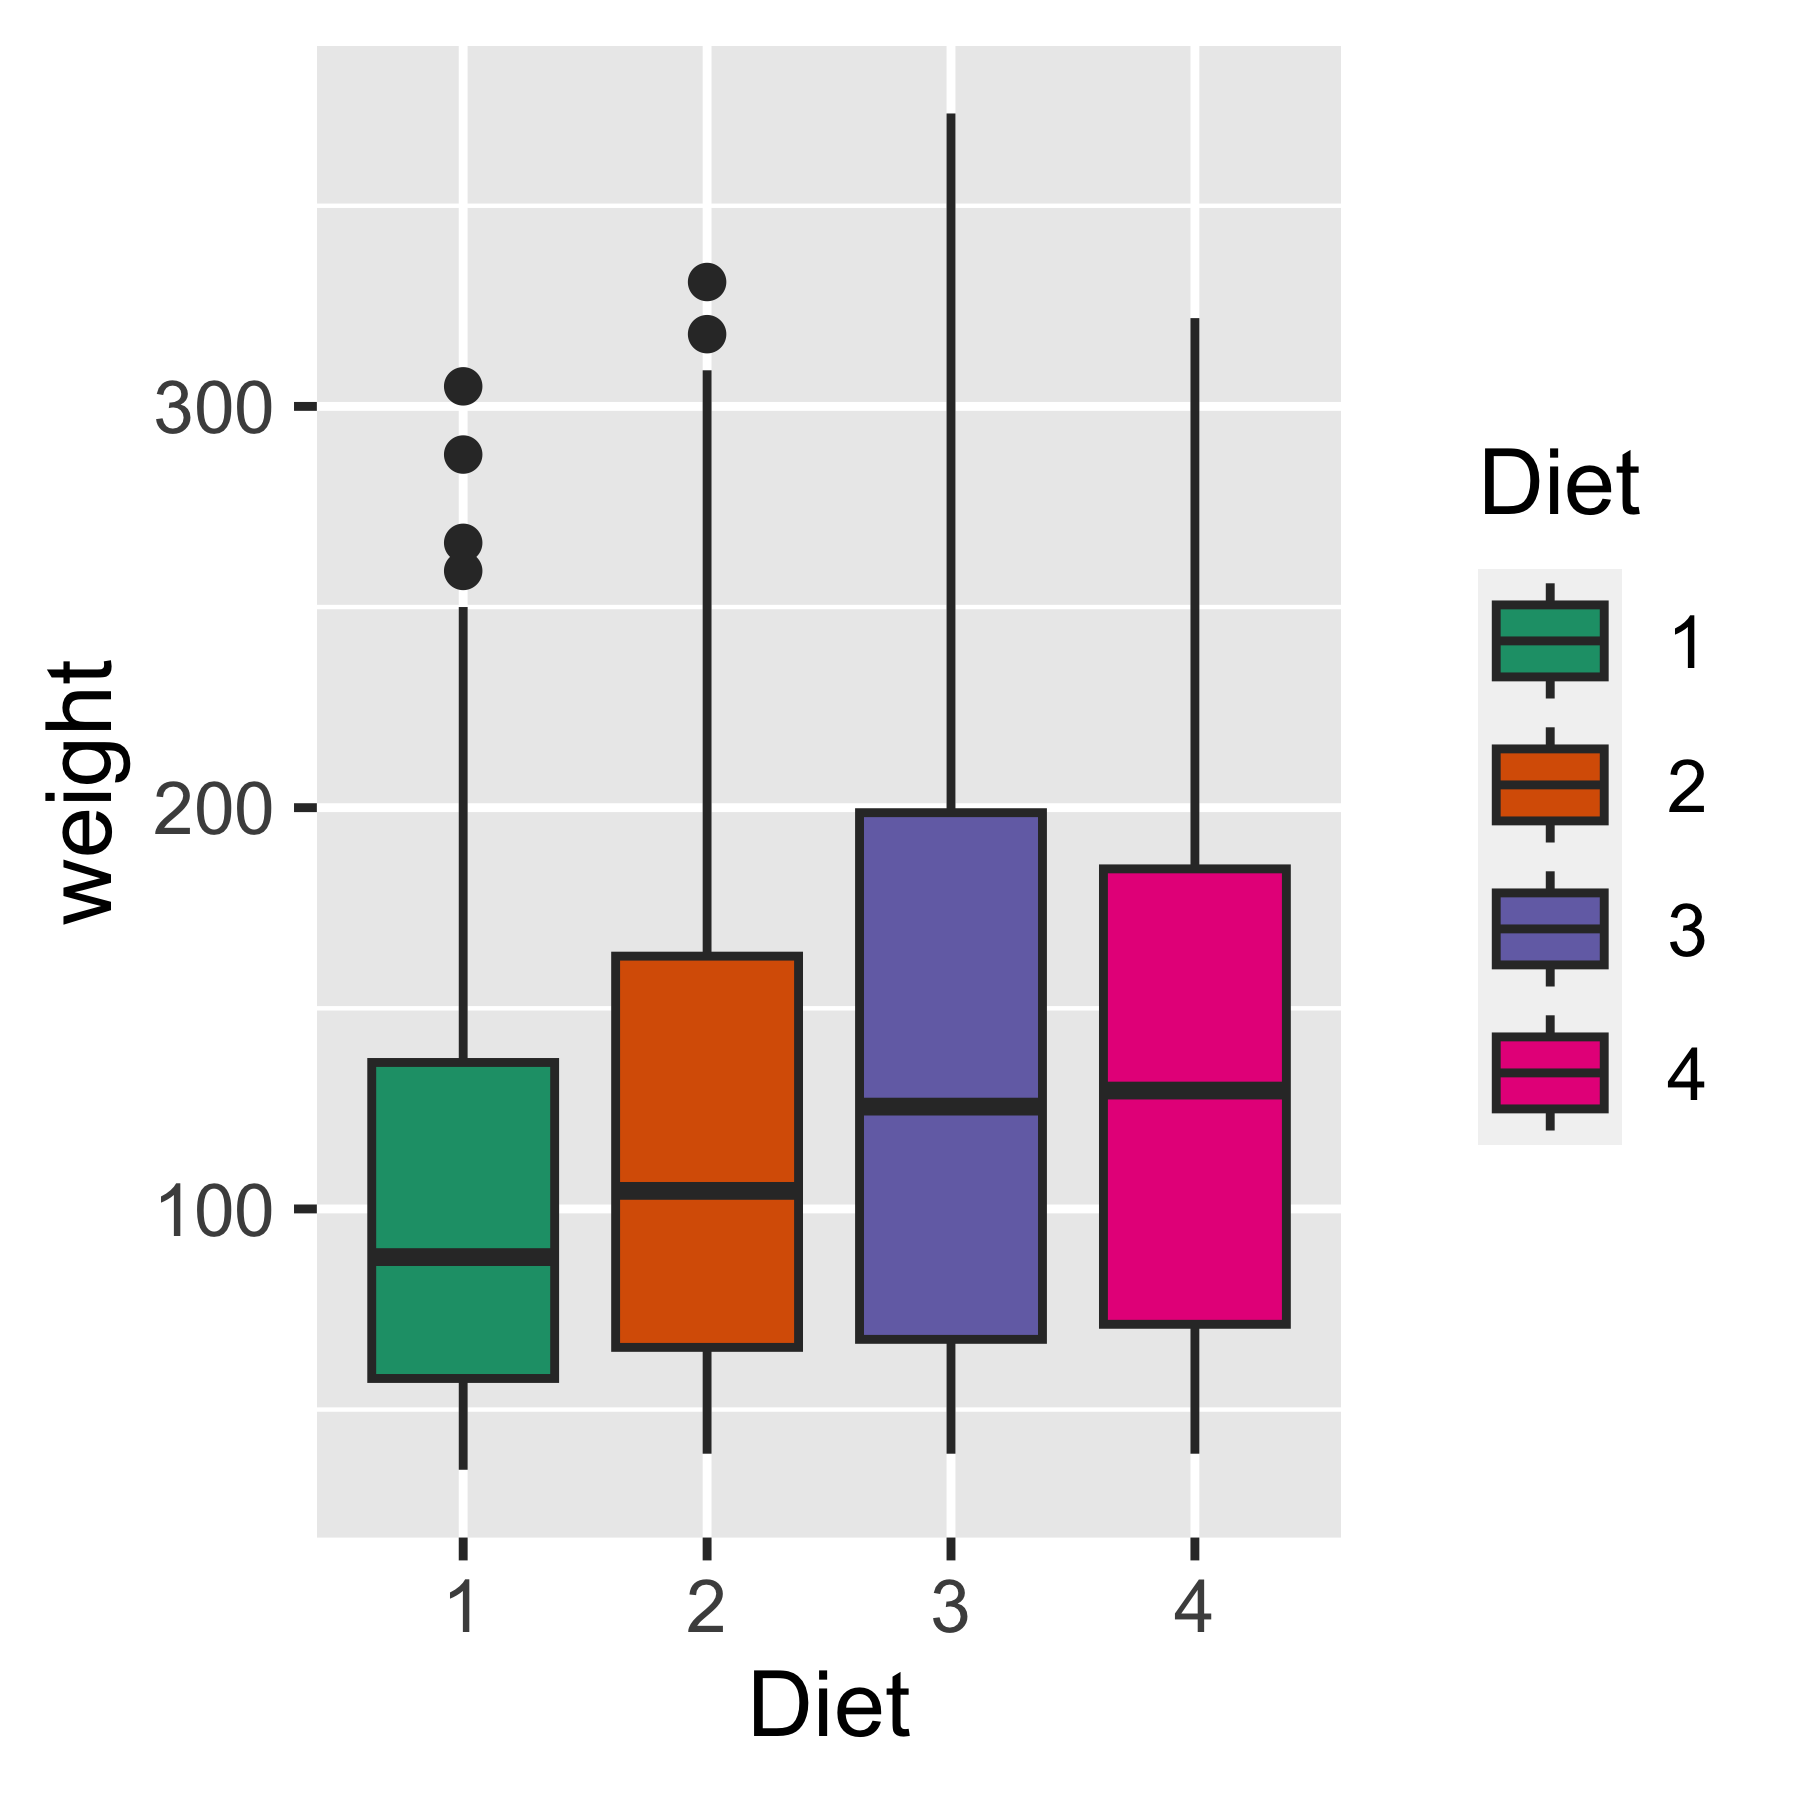
\includegraphics[width=.49\linewidth]{thesis_files/figure-latex/violin_plot-2} \end{center}

Data visualizations are an integral part of the EDA process, enabling analysts to discern patterns and relationships in the data that would otherwise be difficult to discern from tabular data alone.
Through data visualization, analysts can quickly identify trends, outliers, and other patterns that may be missed through numerical analysis alone.
Moreover, visualizations facilitate the communication of findings to non-technical stakeholders, allowing them to comprehend complex data sets more efficiently.
Through visualizations, analysts can also identify potential issues or biases in the data, resulting in better decisions and models.
Thus, visualizations play a crucial role in the EDA process by enabling analysts to more effectively explore, comprehend, and communicate data-derived insights.
During the initial EDA stage, an analyst may find that a variable or a covariate is directly related to the dependent variable when looking at a correlation heatmap or a scatterplot.
The basic understanding can be formalized to visualize the discovery process.

The field of graphical communication, which is directly related to EDA, semiology, and their use in touch, has been a valuable tool and extension of the EDA thoughts that Tukey expressed.
One of the fundamental principles of semiology is the relationship between signifier and signified, in which a visual element (the signifier) represents a particular meaning or concept (the signified), (\textbf{barthes1972?}).
Another essential concept in semiology is using syntax and semantics to convey meaning in graphic communication effectively.
This includes both the syntax and semantics of a graphic's visual elements, (Monmonier, 1985).

Using color to represent data on maps is an example of successful graphical communication utilizing semiology.
By using different colors to represent different data points, viewers can comprehend patterns and relationships in the data quickly and easily.
Jacques Bertin writes in ``Semiology of Graphics'' that color can be used to ``emphasize a point, distinguish one category from another, or establish a relationship between two points'', (Monmonier, 1985).
In addition, Bertin explains that the use of color can help overcome language barriers, making it easier for the audience to comprehend the presented information.

The application of semiology in graphical communication is not devoid of obstacles.
One difficulty is the possibility of misinterpretation, in which viewers may assign a different meaning to a visual element than was intended, (Monmonier, 1985).
Another concern is the possibility of cultural differences in interpretation, in which a visual element may have a different meaning in one culture versus another, (Norman, 2013).

Exploratory Data Analysis (EDA) analyzes and summarizes a dataset to discover patterns, trends, and insights.
It is a crucial step in the data analysis process and is often used to identify which variables are essential, what the data looks like, and what the underlying structure of the data is.
EDA is typically done using various techniques, such as visualizations, statistical summaries, and data transformations.

\hypertarget{open-source-data-suitability-and-integration}{%
\section{Open-Source Data: Suitability and Integration}\label{open-source-data-suitability-and-integration}}

The concept of open source originated long before computers, where shared knowledge formed the basis of human progress.
Originating from the frustrations of figures like Richard Stallman in the 1980s, who championed the free software movement and paved the way for the creation of transformative licenses such as the GNU General Public License, the concept has grown to encompass more than just software. (Stallman, 2002)
With organizations like the Open Source Initiative standardizing open-source practices and monumental projects like Linux showcasing its potential, open-source principles expanded by the late 1990s to include data.
This movement towards openness has been marked by a commitment to transparency, collaboration, and unrestricted access, revolutionizing how we perceive and interact with data in the modern era.
Linux, an open-source operating system kernel initiated by Linus Torvalds in 1991, became one of the most popular examples of open-source success.
The Apache HTTP Server, released in 1995, became another success story, powering a large fraction of the internet (Weber, 2004).
Open-source principles began expanding from software to data in the late 1990s and early 2000s. The idea was to share data sets for public use without restrictions.
Projects like the Human Genome Project advocated for open data to advance science and medicine (Sulston \& Ferry, 2002).

The principles of open-source data revolve around the concepts of free access, transparency, collaboration, and redistribution, fostering a community-driven approach to data sharing and utilization.
At its core, open source is about making the source content (usually software code) freely available.
This transparency allows anyone to review, inspect, and understand the source.
The freedom to use, modify, distribute, and study the source content without restrictions is a cornerstone of open source.
This is articulated in various open source licenses, like the GNU General Public License (GPL), which emphasizes the rights of end users.
Open source projects thrive on collaborative efforts.
Diverse groups of people from around the world contribute, enhancing the project's robustness and creativity.
Tools like Git and platforms like GitHub have made this collaborative approach more streamlined.
Open source projects often foster strong communities.
These communities not only contribute code but also offer support, documentation, and strategies for the project's future.
These communities' sense of belonging and shared purpose is a driving force behind many successful open-source projects.
Contributions to open source projects are often evaluated based on merit.
The best ideas or implementations, regardless of their source, are adopted, promoting a culture of excellence.
The principle of redistribution ensures that modified versions of open source content remain open.
This ensures a perpetual cycle of community-driven improvement and access.
Open source principles prioritize the end user's interests.
This user-centric approach often leads to software or content that's more aligned with what users genuinely need and want.

\hypertarget{open-access-data-repositories}{%
\subsection{Open Access Data Repositories}\label{open-access-data-repositories}}

In the digital age, open access data repositories have become crucial platforms, transforming how data are shared, accessed, and stored among academic and research communities.
These repositories are online spaces created specifically to store datasets and make them available to everyone. In line with the principles of open science, which promote knowledge sharing, transparency, and reproducibility in research endeavors, their main objective is to democratize access to data.

These repositories serve many different purposes at their core.
They support openness in the scientific method first and foremost.
It enables other researchers and the general public to examine, confirm, and replicate research findings by providing unrestricted access to datasets. Collaboration is also encouraged by this open model.
Datasets are accessible to researchers in a variety of fields and locations, providing opportunities to expand upon, combine, or compare various sets of data.
Eliminating research duplication is a significant additional benefit.
Access to data from earlier studies reduces the need to repeatedly collect similar data, which saves time, effort, and resources.
Additionally, these repositories are essential for the long-term preservation of data, guaranteeing that datasets are accessible for future scientific research and for posterity.

A closer look at the features of these repositories reveals several standard components.
Metadata is paramount; this descriptive information elucidates the context, origin, methodology, and other pertinent details of the datasets, ensuring they are comprehensible to those accessing them.
Many repositories also emphasize the citability of datasets.
By assigning a Digital Object Identifier (DOI), datasets become easily referable in academic and research contexts.
Licensing is another cornerstone. To clarify usage rights and conditions, datasets are often accompanied by explicit licenses, with Creative Commons licenses being particularly prevalent.
These licenses can stipulate various conditions, with attribution being a common requirement.
Furthermore, the user experience is enhanced through tools that facilitate easy searching, accessing, and downloading of datasets.

However, like all systems, open access data repositories face challenges.
Ensuring data privacy is a significant concern, especially in datasets derived from human subjects, such as in health or social research.
Standardization is another hurdle.
Given the diverse range of researchers and datasets being uploaded, achieving a standardized format for data and metadata is daunting.
And not to be overlooked is the challenge of sustainability.
Maintaining a sophisticated digital platform requires both financial resources and technical expertise.
Ensuring the longevity of such repositories, especially in a rapidly evolving digital landscape, remains a concern.

Several prominent examples underscore the significance and diversity of open access data repositories.
Zenodo, developed under the European OpenAIRE program, serves as a multifaceted platform catering to researchers across disciplines.
Dryad specializes in datasets linked to scientific publications, predominantly in life sciences and biomedicine.
Figshare offers a broader spectrum, allowing researchers to deposit a range of research outputs, including datasets, making them available to the public.

Historically, the rise of these repositories can be contextualized within the broader open science movement.
This movement, gathering momentum over recent decades, has been advocating for a more transparent, accessible, and shared research process.
As technological advancements surged, leading to an exponential growth in digital data, the emphasis on preserving and sharing this data treasure trove intensified.

Today, the significance of open access data repositories is further underscored by policies and guidelines from influential bodies.
A growing number of funding agencies and academic journals are either mandating or recommending that data underpinning research findings be housed in open access repositories.
This trend not only ensures that research outputs, especially data, remain accessible but also reflects a broader societal push towards transparency, especially when research is funded by public coffers.

\hypertarget{r-package-development---past-present-and-future}{%
\section{R package Development - Past, Present and Future}\label{r-package-development---past-present-and-future}}

R has become a prominent and adaptable programming language within the domain of data analysis and exploratory data analysis (EDA).
A number of R packages have been created to streamline the processes of data manipulation, visualization, and statistical analysis.
One of the prominent programs in this category is \texttt{ggplot2}, which was developed by Hadley Wickham.
This package is widely recognized for its versatility and aesthetic appeal in generating a diverse range of visually appealing and informative data visualizations (\textbf{wickham2016?}).
Wickham et al.~have developed \texttt{dplyr} and \texttt{tidyr}, which offer convenient functionalities for filtering, summarizing, and reshaping data frames, hence enhancing the efficiency of data manipulation activities (\textbf{wickham2021?}).
The \texttt{data.table} package, developed by Matt Dowle, is widely recognized for its remarkable speed and efficiency in handling huge datasets, particularly in the context of performance-oriented data manipulation tasks (\textbf{dowle2021?}).
Although not classified as a R package, it is noteworthy to include Wes McKinney's Python library, \texttt{pandas}, due to its significant influence in the field of data manipulation and analysis in the Python programming language (\textbf{mcKinney2010?}).
Within the field of psychology and psychometrics, the \texttt{psych} package developed by William Revelle serves as an extensive tool for doing factor analysis and reliability analysis (\textbf{revelle202?}).

Furthermore, there are other software packages available that may be utilized by researchers and analysts to enhance their data management and analysis processes.
For instance, the \texttt{naniar} package, developed by (\textbf{tierney2020?}), is specifically designed for handling missing data. Another useful package is \texttt{summarytools}, created by (\textbf{comtois2021?}), which enables the generation of descriptive statistics.
Additionally, the \texttt{corrplot} package, developed by Wei and Simko (Wei et al., 2017), provides significant tools for displaying correlation matrices.
These packages provide researchers and analysts a range of valuable resources to aid in their work.
The \texttt{FactoMineR} package, developed by Husson, Lê, and Pagès (\textbf{husson2020?}), offers crucial techniques for conducting multivariate data analysis, including principal component analysis and clustering.
These software programs, created by renowned individuals in the discipline, jointly provide data analysts and scientists with the necessary tools to efficiently investigate and analyze data.

\hypertarget{dimension-reduction-1}{%
\section{Dimension Reduction}\label{dimension-reduction-1}}

Exploratory Data Analysis (EDA) and Dimension Reduction Techniques are closely intertwined in the realm of data analysis.
EDA serves as the initial step in understanding and visualizing complex datasets, helping analysts uncover patterns, anomalies, and relationships within the data.
However, as datasets grow in dimensionality, the complexity of EDA can become overwhelming. This is where Dimension Reduction Techniques come into play.
By reducing the number of features or variables while preserving the most critical information, these methods simplify the data, making it more manageable for further analysis.
Dimension Reduction Techniques, such as Principal Component Analysis (PCA) or t-Distributed Stochastic Neighbor Embedding (t-SNE), complement EDA by providing a way to condense high-dimensional data into a lower-dimensional space without losing significant insights.
This synergy between EDA and Dimension Reduction Techniques empowers data scientists and analysts to gain deeper insights into their data while efficiently handling large and complex datasets.

\hypertarget{interactive-graphics-1}{%
\section{Interactive Graphics}\label{interactive-graphics-1}}

Interactive graphics are essential to EDA (Unwin, 1999).
Beyond the limitations of static statistical displays, interactive graphics enable visualizations to advance alongside the analysis.
User interaction and direct manipulation are required for dynamic graphics to reach their full potential (Cook et al. (1995); Unwin (1999)).
The connection between EDA and dashboards is that EDA is the process of preparing and understanding the data, which is the first step for building a dashboard, as the data has to be cleaned, transformed, and analyzed to be used efficiently on the dashboard.
EDA results can be used to identify the most relevant data and metrics to include in the dashboard and to design the visualizations that will be used to display the data.
Additionally, the EDA process can identify the outliers, patterns, trends, and insights helpful to show in the dashboard to support decision-making.

Through a multi-phase investigation, this dissertation will:

\begin{enumerate}
\def\labelenumi{\arabic{enumi}.}
\item
  Review the current landscape of dashboard design principles and best practices.
\item
  Analyze the characteristics and quality of open-source data and its suitability for dashboard integration.
\item
  Conduct user-based experiments to determine the challenges and pitfalls naive users face when interacting with dashboards.
\item
  Propose design recommendations for dashboards that effectively convey statistical information to naive users, ensuring correct visual inference and minimizing misinterpretations.
\end{enumerate}

The findings from this research aim to bridge the gap between data experts and naive users, democratizing data interpretation and empowering more individuals to make informed decisions based on open-source data.

\hypertarget{refs}{}
\begin{CSLReferences}{1}{0}
\leavevmode\vadjust pre{\hypertarget{ref-afzal2019}{}}%
Afzal, S., Hittawe, M. M., Ghani, S., Jamil, T., Knio, O., Hadwiger, M., \& Hoteit, I. (2019). The state of the art in visual analysis approaches for ocean and atmospheric datasets. In \emph{Computer graphics forum} (Vol. 38, pp. 881--907). Wiley Online Library.

\leavevmode\vadjust pre{\hypertarget{ref-alabi2012}{}}%
Alabi, O. S., Wu, X., Harter, J. M., Phadke, M., Pinto, L., Petersen, H., et al.others. (2012). Comparative visualization of ensembles using ensemble surface slicing. In \emph{Visualization and data analysis 2012} (Vol. 8294, pp. 318--329). SPIE.

\leavevmode\vadjust pre{\hypertarget{ref-alvarez2011}{}}%
Alvarez, G. A. (2011). Representing multiple objects as an ensemble enhances visual cognition. \emph{Trends in Cognitive Sciences}, \emph{15}(3), 122--131.

\leavevmode\vadjust pre{\hypertarget{ref-alvarez2004}{}}%
Alvarez, G. A., \& Cavanagh, P. (2004). The capacity of visual short-term memory is set both by visual information load and by number of objects. \emph{Psychological Science}, \emph{15}(2), 106--111.

\leavevmode\vadjust pre{\hypertarget{ref-aspillaga1996}{}}%
Aspillaga, M. (1996). Perceptual foundations in the design of visual displays. \emph{Computers in Human Behavior}, \emph{12}(4), 587--600.

\leavevmode\vadjust pre{\hypertarget{ref-baddeley2012}{}}%
Baddeley, A. (2012). Working memory: Theories, models, and controversies. \emph{Annual Review of Psychology}, \emph{63}, 1--29.

\leavevmode\vadjust pre{\hypertarget{ref-baddeley1976}{}}%
Baddeley, Alan D. (1976). \emph{The psychology of memory / alan d. baddeley} (pp. xvii, 430 p. :). Book, Basic Books New York.

\leavevmode\vadjust pre{\hypertarget{ref-bar2004}{}}%
Bar, M. (2004). Visual objects in context. \emph{Nature Reviews Neuroscience}, \emph{5}(8), 617--629.

\leavevmode\vadjust pre{\hypertarget{ref-bauer2009}{}}%
Bauer, B. (2009). Does stevens's power law for brightness extend to perceptual brightness averaging? \emph{The Psychological Record}, \emph{59}, 171--185.

\leavevmode\vadjust pre{\hypertarget{ref-Bendix:2005}{}}%
Bendix, F., Kosara, R., \& Hauser, H. (2005). {Parallel Sets: Visual Analysis of Categorical Data}. In \emph{2005 IEEE symposium on information visualization (INFOVIS'05)} (pp. 133--140). IEEE. http://doi.org/\href{https://doi.org/10.1109/INFOVIS.2005.27}{10.1109/INFOVIS.2005.27}

\leavevmode\vadjust pre{\hypertarget{ref-bland1986}{}}%
Bland, J. M., \& Altman, D. (1986). Statistical methods for assessing agreement between two methods of clinical measurement. \emph{The Lancet}, \emph{327}(8476), 307--310.

\leavevmode\vadjust pre{\hypertarget{ref-bui2014}{}}%
Bui, D. C., \& Myerson, J. (2014). The role of working memory abilities in lecture note-taking. \emph{Learning and Individual Differences}, \emph{33}, 12--22.

\leavevmode\vadjust pre{\hypertarget{ref-cairo2016}{}}%
Cairo, A. (2016). \emph{The truthful art: Data, charts, and maps for communication}. New Riders.

\leavevmode\vadjust pre{\hypertarget{ref-carrillo2019}{}}%
Carrillo-Reid, L., Han, S., Yang, W., Akrouh, A., \& Yuste, R. (2019). Controlling visually guided behavior by holographic recalling of cortical ensembles. \emph{Cell}, \emph{178}(2), 447--457.

\leavevmode\vadjust pre{\hypertarget{ref-chakrabarty2020}{}}%
Chakrabarty, M., \& Wada, M. (2020). Perceptual effects of fast and automatic visual ensemble statistics from faces in individuals with typical development and autism spectrum conditions. \emph{Scientific Reports}, \emph{10}(1), 2169.

\leavevmode\vadjust pre{\hypertarget{ref-chong2003}{}}%
Chong, S. C., \& Treisman, A. (2003). Representation of statistical properties. \emph{Vision Research}, \emph{43}(4), 393--404.

\leavevmode\vadjust pre{\hypertarget{ref-cleveland1984}{}}%
Cleveland, W. S., \& McGill, R. (1984). Graphical perception: Theory, experimentation, and application to the development of graphical methods. \emph{Journal of the American Statistical Association}, \emph{79}(387), 531--554.

\leavevmode\vadjust pre{\hypertarget{ref-cook1995}{}}%
Cook, D., Buja, A., Cabrera, J., \& Hurley, C. (1995). Grand tour and projection pursuit. \emph{Journal of Computational and Graphical Statistics}, \emph{4}(3), 155--172.

\leavevmode\vadjust pre{\hypertarget{ref-corbett2023}{}}%
Corbett, J. E., Utochkin, I., \& Hochstein, S. (2023). \emph{The pervasiveness of ensemble perception: Not just your average review}. Cambridge University Press.

\leavevmode\vadjust pre{\hypertarget{ref-cowan2001}{}}%
Cowan, N. (2001). The magical number 4 in short-term memory: A reconsideration of mental storage capacity. \emph{Behavioral and Brain Sciences}, \emph{24}(1), 87--114.

\leavevmode\vadjust pre{\hypertarget{ref-cowan2010}{}}%
Cowan, N. (2010). The magical mystery four: How is working memory capacity limited, and why? \emph{Current Directions in Psychological Science}, \emph{19}(1), 51--57.

\leavevmode\vadjust pre{\hypertarget{ref-dOcagne:1885}{}}%
d'Ocagne, M. (1885). {Coordonnées parallèles et axiales : Méthode de transformation géométrique et procédé nouveau de calcul graphique déduits de la considération des coordonnées parallèles}. \emph{Gauthier-Villars}, 112. Retrieved from \url{https://archive.org/details/coordonnesparal00ocaggoog/page/n10}

\leavevmode\vadjust pre{\hypertarget{ref-dakin1997}{}}%
Dakin, S. C., \& Watt, R. (1997). The computation of orientation statistics from visual texture. \emph{Vision Research}, \emph{37}(22), 3181--3192.

\leavevmode\vadjust pre{\hypertarget{ref-sine}{}}%
Day, R. H., \& Stecher, E. J. (1991). Sine of an illusion. \emph{Perception}, \emph{20}, 49--55.

\leavevmode\vadjust pre{\hypertarget{ref-dedonno}{}}%
DeDonno, M. A. (2016). The influence of IQ on pure discovery and guided discovery learning of a complex real-world task. \emph{Learning and Individual Differences}, \emph{49}, 11--16.

\leavevmode\vadjust pre{\hypertarget{ref-few2006}{}}%
Few, S. (2006b). \emph{Information dashboard design: The effective visual communication of data}. Newton, MA: O'Reilly Media, Inc.

\leavevmode\vadjust pre{\hypertarget{ref-few}{}}%
Few, S. (2006a). \emph{Information dashboard design: The effective visual communication of data}. Newton, MA: O'Reilly Media, Inc.

\leavevmode\vadjust pre{\hypertarget{ref-fofonov2018}{}}%
Fofonov, A., \& Linsen, L. (2018). A top-down interactive visual analysis approach for physical simulation ensembles at different aggregation levels. \emph{Information}, \emph{9}(7), 163.

\leavevmode\vadjust pre{\hypertarget{ref-goldstein2021}{}}%
Goldstein, E. B., \& Cacciamani, L. (2021). \emph{Sensation and perception, 11th edition}. Cengage Learning.

\leavevmode\vadjust pre{\hypertarget{ref-haberman2019}{}}%
Haberman, J. M., \& Ulrich, L. (2019). Precise ensemble face representation given incomplete visual input. \emph{I-Perception}, \emph{10}(1), 2041669518819014.

\leavevmode\vadjust pre{\hypertarget{ref-haberman2015}{}}%
Haberman, J., Brady, T. F., \& Alvarez, G. A. (2015). Individual differences in ensemble perception reveal multiple, independent levels of ensemble representation. \emph{Journal of Experimental Psychology: General}, \emph{144}(2), 432.

\leavevmode\vadjust pre{\hypertarget{ref-haberman2012}{}}%
Haberman, J., \& Whitney, D. (2012). Ensemble perception: Summarizing the scene and broadening the limits of visual processing. \emph{From Perception to Consciousness: Searching with Anne Treisman}, \emph{33}.

\leavevmode\vadjust pre{\hypertarget{ref-density-pcp}{}}%
Heinrich, J., \& Weiskopf, D. (2009). {Continuous Parallel Coordinates}. \emph{IEEE Transactions on Visualization and Computer Graphics}, \emph{15}(6), 1531--1538. http://doi.org/\href{https://doi.org/10.1109/TVCG.2009.131}{10.1109/TVCG.2009.131}

\leavevmode\vadjust pre{\hypertarget{ref-henderson1999}{}}%
Henderson, J. M., \& Hollingworth, A. (1999). High-level scene perception. \emph{Annual Review of Psychology}, \emph{50}(1), 243--271.

\leavevmode\vadjust pre{\hypertarget{ref-Hofmann:2013}{}}%
Hofmann, H., \& Vendettuoli, M. (2013). {Common Angle Plots as Perception-True Visualizations of Categorical Associations}. \emph{IEEE Transactions on Visualization and Computer Graphics}, \emph{19}(12), 2297--2305. http://doi.org/\href{https://doi.org/10.1109/TVCG.2013.140}{10.1109/TVCG.2013.140}

\leavevmode\vadjust pre{\hypertarget{ref-hubel2004}{}}%
Hubel, D. H., \& Wiesel, T. N. (2004). \emph{Brain and visual perception: The story of a 25-year collaboration}. Oxford University Press.

\leavevmode\vadjust pre{\hypertarget{ref-hullman2011}{}}%
Hullman, J., Adar, E., \& Shah, P. (2011). Benefitting infovis with visual difficulties. \emph{IEEE Transactions on Visualization and Computer Graphics}, \emph{17}(12), 2213--2222.

\leavevmode\vadjust pre{\hypertarget{ref-hullman2021}{}}%
Hullman, J., \& Gelman, A. (2021). Designing for {Interactive} {Exploratory} {Data} {Analysis} {Requires} {Theories} of {Graphical} {Inference}. \emph{Harvard Data Science Review}, \emph{3}(3).

\leavevmode\vadjust pre{\hypertarget{ref-itti2000}{}}%
Itti, L., \& Koch, C. (2000). A saliency-based search mechanism for overt and covert shifts of visual attention. \emph{Vision Research}, \emph{40}(10-12), 1489--1506.

\leavevmode\vadjust pre{\hypertarget{ref-JHUCovidDashboard}{}}%
John hopkins university covid-19 dashboard. (n.d.). Retrieved from \url{https://coronavirus.jhu.edu/map.html}

\leavevmode\vadjust pre{\hypertarget{ref-karjus2023}{}}%
Karjus, A., Solà, M. C., Ohm, T., Ahnert, S. E., \& Schich, M. (2023). Compression ensembles quantify aesthetic complexity and the evolution of visual art. \emph{EPJ Data Science}, \emph{12}(1), 21.

\leavevmode\vadjust pre{\hypertarget{ref-khayat2023}{}}%
Khayat, N., Ahissar, M., \& Hochstein, S. (2023). Perceptual history biases in serial ensemble representation. \emph{Journal of Vision}, \emph{23}(3), 7--7.

\leavevmode\vadjust pre{\hypertarget{ref-khayat2021}{}}%
Khayat, N., Fusi, S., \& Hochstein, S. (2021). Perceiving ensemble statistics of novel image sets. \emph{Attention, Perception, \& Psychophysics}, \emph{83}, 1312--1328.

\leavevmode\vadjust pre{\hypertarget{ref-khayat2018}{}}%
Khayat, N., \& Hochstein, S. (2018). Perceiving set mean and range: Automaticity and precision. \emph{Journal of Vision}, \emph{18}(9), 23--23.

\leavevmode\vadjust pre{\hypertarget{ref-leavitt2017}{}}%
Leavitt, M. L., Pieper, F., Sachs, A. J., \& Martinez-Trujillo, J. C. (2017). Correlated variability modifies working memory fidelity in primate prefrontal neuronal ensembles. \emph{Proceedings of the National Academy of Sciences}, \emph{114}(12), E2494--E2503.

\leavevmode\vadjust pre{\hypertarget{ref-lee}{}}%
Lee, S., Kim, S.-H., Hung, Y.-H., Lam, H., Kang, Y., \& Yi, J. S. (2016). How do people make sense of unfamiliar visualizations?: A grounded model of novice's information visualization sensemaking. \emph{IEEE}, \emph{22}, 499--508.

\leavevmode\vadjust pre{\hypertarget{ref-leib2016}{}}%
Leib, A. Y., Kosovicheva, A., \& Whitney, D. (2016). Fast ensemble representations for abstract visual impressions. \emph{Nature Communications}, \emph{7}(1), 13186.

\leavevmode\vadjust pre{\hypertarget{ref-luxen-vetter-2011}{}}%
Luxen, D., \& Vetter, C. (2011). Real-time routing with OpenStreetMap data. In \emph{Proceedings of the 19th ACM SIGSPATIAL international conference on advances in geographic information systems} (pp. 513--516). New York, NY, USA: ACM. http://doi.org/\href{https://doi.org/10.1145/2093973.2094062}{10.1145/2093973.2094062}

\leavevmode\vadjust pre{\hypertarget{ref-maule2015}{}}%
Maule, J., \& Franklin, A. (2015). Effects of ensemble complexity and perceptual similarity on rapid averaging of hue. \emph{Journal of Vision}, \emph{15}(4), 6--6.

\leavevmode\vadjust pre{\hypertarget{ref-attention}{}}%
McCallum, W. C. (n.d.). Attention. \url{https://www.britannica.com/science/attention}.

\leavevmode\vadjust pre{\hypertarget{ref-bertin1983}{}}%
Monmonier, M. (1985). \emph{Annals of the Association of American Geographers}, \emph{75}(4), 605--609. Retrieved from \url{http://www.jstor.org/stable/2563117}

\leavevmode\vadjust pre{\hypertarget{ref-elsi}{}}%
National Center for Education Statistics. (2020). National center for education statistics. \url{https://nces.ed.gov/}.

\leavevmode\vadjust pre{\hypertarget{ref-norman2013}{}}%
Norman, D. (2013). \emph{The design of everyday things: Revised and expanded edition}. Basic books.

\leavevmode\vadjust pre{\hypertarget{ref-oberauer2009}{}}%
Oberauer, K. (2009). Design for a working memory. \emph{Psychology of Learning and Motivation}, \emph{51}, 45--100.

\leavevmode\vadjust pre{\hypertarget{ref-padilla2017}{}}%
Padilla, L. M., Ruginski, I. T., \& Creem-Regehr, S. H. (2017). Effects of ensemble and summary displays on interpretations of geospatial uncertainty data. \emph{Cognitive Research: Principles and Implications}, \emph{2}, 1--16.

\leavevmode\vadjust pre{\hypertarget{ref-palmer2002}{}}%
Palmer, S. E. (2002). Perceptual organization in vision. \emph{Stevens' Handbook of Experimental Psychology}.

\leavevmode\vadjust pre{\hypertarget{ref-perez2021}{}}%
Pérez-Ortega, J., Alejandre-Garcı́a, T., \& Yuste, R. (2021). Long-term stability of cortical ensembles. \emph{Elife}, \emph{10}, e64449.

\leavevmode\vadjust pre{\hypertarget{ref-petersCommunityResiliencyDeclining2019}{}}%
Peters, D. J. (2019). Community {Resiliency} in {Declining} {Small} {Towns}: {Impact} of {Population} {Loss} on {Quality} of {Life} over 20 {Years}. \emph{Rural Sociology}, \emph{84}(4), 635--668. http://doi.org/\href{https://doi.org/10.1111/ruso.12261}{10.1111/ruso.12261}

\leavevmode\vadjust pre{\hypertarget{ref-playfair2005}{}}%
Playfair, W. (2005). \emph{Playfair's commercial and political atlas and statistical breviary}. Cambridge University Press.

\leavevmode\vadjust pre{\hypertarget{ref-potter2009}{}}%
Potter, K., Wilson, A., Bremer, P.-T., Williams, D., Doutriaux, C., Pascucci, V., \& Johnson, C. R. (2009). Ensemble-vis: A framework for the statistical visualization of ensemble data. In \emph{2009 IEEE international conference on data mining workshops} (pp. 233--240). IEEE.

\leavevmode\vadjust pre{\hypertarget{ref-r}{}}%
R Core Team. (2022). \emph{R: A language and environment for statistical computing}. Vienna, Austria: R Foundation for Statistical Computing. Retrieved from \url{https://www.R-project.org/}

\leavevmode\vadjust pre{\hypertarget{ref-rayner2009}{}}%
Rayner, K. (2009). The 35th sir frederick bartlett lecture: Eye movements and attention in reading, scene perception, and visual search. \emph{Quarterly Journal of Experimental Psychology}, \emph{62}(8), 1457--1506.

\leavevmode\vadjust pre{\hypertarget{ref-rubin2008}{}}%
Rubin, J., \& Chisnell, D. (2008). \emph{Handbook of usability testing: How to plan, design, and conduct effective tests}. John Wiley \& Sons.

\leavevmode\vadjust pre{\hypertarget{ref-scc}{}}%
Rural Shrink Smart Team. (2022). Rural shrink smart. \url{https://ruralshrinksmart.org/}.

\leavevmode\vadjust pre{\hypertarget{ref-fisher}{}}%
Sarikaya, A., Correll, M., Bartram, L., Tory, M., \& Fisher, D. (2019). What do we talk about when we talk about dashboards? \emph{IEEE Transactions on Visualization and Computer Graphics}, \emph{25}(1), 682--692. http://doi.org/\href{https://doi.org/10.1109/TVCG.2018.2864903}{10.1109/TVCG.2018.2864903}

\leavevmode\vadjust pre{\hypertarget{ref-satyanarayan2016}{}}%
Satyanarayan, A., Moritz, D., Wongsuphasawat, K., \& Heer, J. (2016). Vega-lite: A grammar of interactive graphics. \emph{IEEE Transactions on Visualization and Computer Graphics}, \emph{23}(1), 341--350.

\leavevmode\vadjust pre{\hypertarget{ref-schwendimann2016}{}}%
Schwendimann, B. A., Rodriguez-Triana, M. J., Vozniuk, A., Prieto, L. P., Boroujeni, M. S., Holzer, A., \ldots{} Dillenbourg, P. (2016). Perceiving learning at a glance: A systematic literature review of learning dashboard research. \emph{IEEE Transactions on Learning Technologies}, \emph{10}(1), 30--41.

\leavevmode\vadjust pre{\hypertarget{ref-stallman2002}{}}%
Stallman, R. (2002). \emph{Free software, free society: Selected essays of richard m. stallman}. Lulu. com.

\leavevmode\vadjust pre{\hypertarget{ref-iowa_gov}{}}%
State of Iowa. (2020). Iowa data portal. \url{https://data.iowa.gov}.

\leavevmode\vadjust pre{\hypertarget{ref-sulston2002}{}}%
Sulston, J., \& Ferry, G. (2002). \emph{The common thread: A story of science, politics, ethics, and the human genome}. Random House.

\leavevmode\vadjust pre{\hypertarget{ref-szafir2017}{}}%
Szafir, D. A. (2017). Modeling color difference for visualization design. \emph{IEEE Transactions on Visualization and Computer Graphics}, \emph{24}(1), 392--401.

\leavevmode\vadjust pre{\hypertarget{ref-szafir2016}{}}%
Szafir, D. A., Haroz, S., Gleicher, M., \& Franconeri, S. (2016). Four types of ensemble coding in data visualizations. \emph{Journal of Vision}, \emph{16}(5), 11--11.

\leavevmode\vadjust pre{\hypertarget{ref-treisman1998}{}}%
Treisman, A. (1998). Feature binding, attention and object perception. \emph{Philosophical Transactions of the Royal Society of London. Series B: Biological Sciences}, \emph{353}(1373), 1295--1306.

\leavevmode\vadjust pre{\hypertarget{ref-treisman1980}{}}%
Treisman, A. M., \& Gelade, G. (1980). A feature-integration theory of attention. \emph{Cognitive Psychology}, \emph{12}(1), 97--136.

\leavevmode\vadjust pre{\hypertarget{ref-tufte1985}{}}%
Tufte, Edward R. (1985). The visual display of quantitative information. \emph{The Journal for Healthcare Quality (JHQ)}, \emph{7}(3), 15.

\leavevmode\vadjust pre{\hypertarget{ref-tufte2001}{}}%
Tufte, Edward R. (2001). \emph{The visual display of quantitative information (2nd edition)}. USA: Graphics Press.

\leavevmode\vadjust pre{\hypertarget{ref-tukey1966}{}}%
Tukey, J. W., \& Wilk, M. B. (1966). Data analysis and statistics: An expository overview. In \emph{Proceedings of the november 7-10, 1966, fall joint computer conference} (pp. 695--709).

\leavevmode\vadjust pre{\hypertarget{ref-unwin1999}{}}%
Unwin, A. (1999). Requirements for interactive graphics software for exploratory data analysis. \emph{Computational Statistics}, \emph{14}(1), 7--22.

\leavevmode\vadjust pre{\hypertarget{ref-unwin2003}{}}%
Unwin, A., Volinsky, C., \& Winkler, S. (2003). Parallel coordinates for exploratory modelling analysis. \emph{Computational Statistics \& Data Analysis}, \emph{43}, 553--564. http://doi.org/\href{https://doi.org/10.1016/S0167-9473(02)00292-X}{10.1016/S0167-9473(02)00292-X}

\leavevmode\vadjust pre{\hypertarget{ref-Rural_classification}{}}%
USDA - ERS. (2020a). Rural classifications. \url{https://www.ers.usda.gov/topics/rural-economy-population/rural-classifications/}.

\leavevmode\vadjust pre{\hypertarget{ref-usda}{}}%
USDA - ERS. (2020b). Rural-urban commuting area codes. \url{https://www.ers.usda.gov/data-products/rural-urban-commuting-area-codes/}.

\leavevmode\vadjust pre{\hypertarget{ref-utochkin2023}{}}%
Utochkin, I. S., Choi, J., \& Chong, S. C. (2023). A population response model of ensemble perception. \emph{Psychological Review}.

\leavevmode\vadjust pre{\hypertarget{ref-sineillusion}{}}%
VanderPlas, S., \& Hofmann, H. (2015a). Signs of the sine illusion--why we need to care. \emph{Journal of Computational and Graphical Statistics}, \emph{24}(4), 1170--1190. http://doi.org/\href{https://doi.org/10.1080/10618600.2014.951547}{10.1080/10618600.2014.951547}

\leavevmode\vadjust pre{\hypertarget{ref-vanderplas2015}{}}%
VanderPlas, S., \& Hofmann, H. (2015b). Signs of the sine illusion---why we need to care. \emph{Journal of Computational and Graphical Statistics}, \emph{24}(4), 1170--1190.

\leavevmode\vadjust pre{\hypertarget{ref-wagemans2012}{}}%
Wagemans, J., Feldman, J., Gepshtein, S., Kimchi, R., Pomerantz, J. R., Van der Helm, P. A., \& Van Leeuwen, C. (2012). A century of gestalt psychology in visual perception: II. Conceptual and theoretical foundations. \emph{Psychological Bulletin}, \emph{138}(6), 1218.

\leavevmode\vadjust pre{\hypertarget{ref-ward2010}{}}%
Ward, M., Grinstein, G., \& Keim, D. (2010). \emph{Interactive data visualization: Foundations, techniques, and applications} (p. 81). http://doi.org/\href{https://doi.org/10.1201/b10683}{10.1201/b10683}

\leavevmode\vadjust pre{\hypertarget{ref-ware2012}{}}%
Ware, C. (2012). \emph{Information visualization: Perception for design}. Morgan Kaufmann.

\leavevmode\vadjust pre{\hypertarget{ref-weber2004}{}}%
Weber, S. (2004). \emph{The success of open source}. Harvard University Press.

\leavevmode\vadjust pre{\hypertarget{ref-wei2017}{}}%
Wei, T., Simko, V., Levy, M., Xie, Y., Jin, Y., Zemla, J., et al. (2017). Package {``corrplot.''} \emph{Statistician}, \emph{56}(316), e24.

\leavevmode\vadjust pre{\hypertarget{ref-wertheimer1912}{}}%
Wertheimer, M. (1912). Experimentelle studien uber das sehen von bewegung (translated extract reprinted as {``experimental studies on the seeing of motion''}). \emph{Zeitschrift Fur Psychologie}, \emph{61}, 161--165.

\leavevmode\vadjust pre{\hypertarget{ref-wertheimer1923}{}}%
WERTHEIMER, M. (1923). Laws of organization in perceptual forms. First published as untersuchungen zur lehre von der gestalt II. \emph{Psychologische Forschung}, \emph{4}, 301--350.

\leavevmode\vadjust pre{\hypertarget{ref-wertheimer1938}{}}%
Wertheimer, M. (1938). Laws of organization in perceptual forms.

\leavevmode\vadjust pre{\hypertarget{ref-whitney2014}{}}%
Whitney, D., Haberman, J., \& Sweeny, T. D. (2014). 49 from textures to crowds: Multiple levels of summary statistical perception. \emph{The New Visual Neurosciences}, 695--710.

\leavevmode\vadjust pre{\hypertarget{ref-whitney2022}{}}%
Whitney, D., \& Manassi, M. (2022). Ensemble perception: Stacking the hay to find the needle. \emph{Current Biology}, \emph{32}(22), R1264--R1266.

\leavevmode\vadjust pre{\hypertarget{ref-ggplot2}{}}%
Wickham, H. (2016). \emph{{ggplot2: Elegant Graphics for Data Analysis}} (2nd ed.). Springer-Verlag New York. Retrieved from \url{https://ggplot2.tidyverse.org}

\leavevmode\vadjust pre{\hypertarget{ref-tourr}{}}%
Wickham, H., Cook, D., Hofmann, H., \& Buja, A. (2011). {tourr: An R Package for Exploring Multivariate Data with Projections}. \emph{Journal of Statistical Software, Articles}, \emph{40}(2), 1--18. http://doi.org/\href{https://doi.org/10.18637/jss.v040.i02}{10.18637/jss.v040.i02}

\leavevmode\vadjust pre{\hypertarget{ref-wilkinson2012}{}}%
Wilkinson, L. (2012). \emph{The grammar of graphics}. Springer.

\leavevmode\vadjust pre{\hypertarget{ref-zarecor2021rural}{}}%
Zarecor, K. E., Peters, D. J., \& Hamideh, S. (2021). Rural smart shrinkage and perceptions of quality of life in the american midwest. In \emph{Handbook of quality of life and sustainability} (pp. 395--415). Springer.

\end{CSLReferences}


%% backmatter is needed at the end of the main body of your thesis to
%% set up page numbering correctly for the remainder of the thesis
\backmatter

%% Start the correct formatting for the appendices
% \appendix
%% Input each appendix here
% \input{./appendix_a}

%% Bibliography goes here (You better have one)
%% BibTeX is your friend

% \bibliographystyle{alpha}  % or use  abbrv to abbreviate first names and use numerical indices
\bibliographystyle{abbrv}  % or use  abbrv to abbreviate first names and use numerical indices
%% Add your BibTex file here (don't include the .bib)
\bibliography{./references}



%% Index go here (if you have one)
\end{document}
